\documentclass[10pt, a4paper]{report}

% Language setting
\usepackage[english]{babel}

\usepackage[a4paper]{geometry}

% Useful packages
\usepackage{amsmath}
\usepackage{amssymb}
\usepackage{amsthm}
\usepackage{mathtools}
\usepackage{graphicx}
\usepackage{mathrsfs}
\usepackage{mathtools}
\usepackage{xcolor}
\usepackage{setspace}
\usepackage{tikz-cd}
\usepackage{pgfgantt}
\usepackage[backend=bibtex,firstinits=true]{biblatex}
\usepackage[colorlinks=true, allcolors=blue]{hyperref}
\usepackage{enumitem}
\setenumerate{itemsep=-2mm}
\usepackage{parskip}
\setlength{\parindent}{15pt}
\usepackage{fancyhdr}

\usepackage{cleveref}

\theoremstyle{definition}
\newtheorem{theorem}{Theorem}
\newtheorem{corollary}[theorem]{Corollary}
\newtheorem{lemma}[theorem]{Lemma}
\newtheorem{prop}[theorem]{Proposition}
\newtheorem{defn}[theorem]{Definition}
\newtheorem{example}[theorem]{Example}
\numberwithin{theorem}{section}

\linespread{1.18}

\pagestyle{fancy}
\fancyhf{}
\fancyhead[L]{\nouppercase{\leftmark}}
\fancyhead[L]{\nouppercase{\rightmark}}
\fancyfoot[C]{\thepage}

\newcommand{\resfield}{\mathscr{H}(x)}
\newcommand{\resfieldof}[1]{\mathscr{H}(#1)}
\newcommand{\resresfield}{\widetilde{\mathscr{H}}(x)}
\newcommand{\affline}{\mathbb{A}^{1, \text{an}}_{k}}
\newcommand{\affnspace}{\mathbb{A}^{n, \text{an}}_{k}}
\newcommand{\projlinean}{\mathbb{P}^{1, \text{an}}_{k}}
\newcommand{\projplanean}{\mathbb{P}^{2, \text{an}}_{k}}
\newcommand{\berkspec}[1]{\mathcal{M}\left(#1\right)}
\newcommand{\berkspeck}[1]{\mathcal{M}\left(k\{#1\}\right)}
\newcommand{\berkspect}[1]{\mathcal{M}(#1)}
\newcommand{\berkunitdisk}{\mathcal{M}(k\{T\})}
\newcommand{\tatealgr}{k\{r^{-1}T\}}
\newcommand{\kaff}{$k$-$\mathcal{A}\textit{ff}$ }
\newcommand{\kanl}{$k$-$\mathcal{A}n$ }
\newcommand{\spf}[1]{\operatorname{Spf} #1}
\newcommand{\red}[2]{\operatorname{red}_{#1}(#2)}
\newcommand{\redi}[2]{\operatorname{red}^{#1}(#2)}
\newcommand{\model}{\mathscr{X}}
\newcommand{\fmodel}{\mathfrak{X}}
\newcommand{\blowup}[2]{\operatorname{Bl}_{#2}#1}
\newcommand{\torusan}{\mathbb{G}^{\text{an}}_{m, k}}
\newcommand{\evt}{\operatorname{ev}_{T}}
\newcommand{\annulus}[1]{\mathbb{S}(#1)}
\newcommand{\resfieldan}{\mathscr{H}^{\text{an}}(x)}
\newcommand{\op}[1]{#1^{\operatorname{op}}}
\newcommand{\divisor}{\operatorname{div}}

\newcommand{\spec}{\operatorname{Spec}}
\newcommand{\proj}{\operatorname{Proj}}
\newcommand{\sheaf}{\mathcal{O}}
\newcommand{\trop}{\operatorname{trop}}
\newcommand{\val}{\operatorname{val}}
\newcommand{\sk}[1]{\operatorname{Sk}(#1)}
\newcommand{\maxideal}{\mathfrak{m}}

\newcommand{\RR}{\mathbb{R}}
\newcommand{\QQ}{\mathbb{Q}}
\newcommand{\NN}{\mathbb{N}}
\newcommand{\ZZ}{\mathbb{Z}}
\newcommand{\CC}{\mathbb{C}}

\newcommand{\banr}{\mathscr{A}}
\newcommand{\banb}{\mathscr{B}}
\newcommand{\norm}{||\cdot||}
\newcommand{\snorm}{|\cdot|}
\newcommand{\absval}{|\cdot|}
\newcommand{\snormx}{|\cdot|_x}

\newcommand{\anl}[1]{#1^{\text{an}}}


\title{The Geometry of Berkovich Analytic Spaces}
\author{Aporva Varshney \\ Supervisor: Professor Johannes Nicaise \\ Second Marker: Professor Alexei Skorobogatov}
\date{2022}
\addbibresource{refs}

\begin{document}

\maketitle

\begin{abstract}
    The $p$-adic fields $\mathbb{Q}_p$ are integral in number theory and arithmetic geometry, and serve as a key example of a non-Archimedean field.
    Unfortunately, a na{\"i}ve attempt to construct a theory of analytic geometry over $\mathbb{Q}_p$, paralleling the one over the complex numbers $\mathbb{C}$, fails to be useful. 
    For example, a compact analytic manifold over $\mathbb{Q}_p$ decomposes as a disjoint union of open balls.
    Over $\mathbb{C}$, algebraic objects such as curves given by the zero sets of polynomials may be studied as analytic objects by considering their analytifications.
    Such analytifications reflect the geometry of the algebraic object, but an analog over $\mathbb{Q}_p$ using only the na{\"i}ve approach lacks this property due to the highly disconnected nature of compact manifolds.
    
    Berkovich spaces provide an alternative approach to non-Archimedean analytic geometry, giving a topologically well-behaved class of spaces.
    They allow for analytifications of varieties over non-Archimedean fields, which preserve several important properties of the geometry of the variety.
    This project aims to serve as an introduction to the theory of these spaces and how their geometric properties may be determined, illustrating the theory with several examples, including the case of elliptic curves.
    Of particular importance is the notion of a skeleton of a Berkovich space, which is a subspace controlling the homotopy type of the space.
    We study how skeleta may be found for both curves and higher dimensional spaces. 
    In particular, we give a proof of a result showing how a Berkovich space may be recovered as a topological inverse limit of its skeleta.
    To the best of our knowledge, all proofs of this result in the literature utilise more advanced techniques in algebraic geometry than those in this report; the proof given here can be considered more direct and explicit.
\end{abstract}

\tableofcontents


\chapter{Introduction}

\section{Motivation}

A field $k$ is said to be non-Archimedean with respect to an absolute value  ${\absval: k \to \RR}$ if the ultrametric triangle inequality is satisfied:
\[
|f + g| \leq \max\{|f|, |g|\} \; \; \; \; \; \forall f, g \in k.
\]
In number theory, a prominent example of such fields are the $p$-adics $\QQ_p$ equipped with the $p$-adic absolute value, while in geometry, one is often interested in working over the field of Laurent series $F((t))$ over a field $F$, equipped with the $t$-adic absolute value.

Over $\CC$, an important class of geometric objects comes in the form of Riemann surfaces, which are compact analytic manifolds of complex dimension $1$. 
More generally, a nonsingular variety over $\CC$ admits an analytification, which is a complex analytic space; Riemann surfaces then correspond to analytifications of curves. 
Furthermore, the analytification of a variety may be studied using \textit{transcendental methods} (see \parencite[Appendix B]{hartshorne}).
A suitable GAGA principle then indicates that the geometry of the analytification reflects the geometry of the original variety.

In order to develop a similar theory over non-Archimedean fields, it is natural to consider compact analytic manifolds, but here, a theorem of Serre shows that such spaces are poorly behaved when the base field is non-Archimedean and locally compact - as is the case for the fields $\QQ_p$ and $\mathbb{F}_q((t))$.

\begin{theorem}\parencite[Appendix 2]{serre}
    Let $X$ be a non-empty, compact analytic manifold over a locally compact and non-Archimedean field. Then $X$ decomposes as a disjoint union of a finite number of balls. If there are two such decompositions into $n$ and $m$ balls respectively, then $n \equiv m \mod q$, where $q$ is the size of the residue field.
\end{theorem}

In particular, this completely determines the structure of any such manifold and motivates the need for an improved notion of non-Archimedean analytic spaces. 

An important milestone in the development of a well-behaved non-Archimedean analytic theory came through Tate's rigid analytic spaces in the 1960s. 
These spaces, developed using rings of convergent power series as opposed to the polynomial rings used in algebraic geometry, were much better behaved, admitting, for example, a suitable GAGA principle. 
An important variation, and the one which will be principally studied here, was in the form of Berkovich's $k$-analytic spaces, developed in the late 1980s.
An advantage offered by Berkovich spaces was that it became possible to work directly with the topology of the space itself, as opposed to the `Grothendieck topology' used in rigid analytic geometry, a feat made possible by effectively adding additional points to rigid spaces.
Presently, Berkovich spaces find a plethora of uses, including non-Archimedean analogues for potential theory \parencite{potdynams} and mirror symmetry \parencite{kontsevich, vietnam}.

\section{Report Structure}

In this report, we explore the theory of Berkovich spaces, focusing on techniques to visualise and determine the geometry of such spaces. 
We assume some knowledge of algebraic geometry, category theory and some elementary results in non-Archimedean analysis. 
In particular, it is crucial to use the theory of schemes as opposed to the classical theory of varieties.

In the first core chapter, we review the construction of Berkovich spaces.
Although there are some parallels here with the construction of schemes, some more care is needed in comparison with the approach taken in algebraic geometry, since we must additionally capture the analytic aspects of the rings that we are working with.
The primary example considered to illustrate the theory is that of the analytic affine line $\affline$, for which we are able to derive an explicit picture.
We also describe the construction of the analytification functor, assigning to a $k$-variety $X$ the Berkovich space $\anl{X}$.

We then focus our attention towards $k$-analytic curves.
We give an overview of formal schemes and formal models.
In general, a model for an analytic space can be considered to be a space, such as a scheme or a formal scheme, which captures the geometry of the analytic space. 
Then, we move on to the notion of a skeleton, which is a fundamental concept in the theory of Berkovich spaces.
If $X$ is a $k$-analytic space, then a skeleton $\Sigma$ is a closed subset of $X$ admitting a strong deformation retraction $X \to \Sigma$.
In particular, the homotopy type of $X$ is controlled by the skeleton.
We see how skeleta of curves are closely linked to the classical theory of semistable formal models, using the analytic projective line to illustrate the correspondence.

Equipped with the ideas and imagery of curves, we then generalise the notion of a skeleton to higher dimensional analytic spaces.
For each proper variety $X$ over $k$, we consider the class of schemes which model the analytic space $\anl{X}$, known as snc models.
We see how an snc model $\model$ gives rise to a skeleton $\sk{\model} \subset \anl{X}$, and furthermore, provide a proof of \cref{thm:homeomorphism}, which states that there is a homeomorphism
\[
    \anl{X} \cong \varprojlim \sk{\model}
\]
as $\model$ ranges over the snc models of $\anl{X}$.
Informally, the topology of $\anl{X}$ is determined by its snc models.

In the final chapter, we consider the case of elliptic curves, explaining how non-Archimedean uniformization theory may be used to construct the analytic space associated to an elliptic curve with multiplicative reduction.
We apply the results from previous chapters to compute skeleta for this space.

\subsection{Contributions}

The contributions of the report are summarised as follows.
\begin{itemize}
    \item Various aspects of the theory originally spread across various textbooks and papers are organised into one report.
    In particular, there is no standard textbook for non-Archimedean geometry, so information has been consolidated from a variety of sources.
    \item Examples in addition to what is presented in the sources have been computed in order to better illustrate the theory.
    \item Efforts have been made to clarify details and arguments which were omitted in the original sources or left as exercises to the reader.
    \item A proof is given of the result labelled in the following chapters as \cref{thm:homeomorphism}. 
    To the best of our knowledge, proofs in the literature of this result require more advanced techniques in algebraic geometry  (see \parencite{bfj}).
    We present two proofs for this result which essentially depend only on standard results on blow-ups of schemes, hence providing a more direct and explicit argument.
        \begin{itemize}
            \item The first proof works for arbitrary dimensions, but requires resolution of singularities, which is a powerful result in birational geometry.
            \item The second proof does not depend on resolution of singularities, but works only in the case of curves.
        \end{itemize}
\end{itemize}

\paragraph{Notation and Conventions}

Throughout the report, $k$ will denote a complete non-Archimedean field with a non-trivial absolute value $|\cdot|$.
Its valuation ring will be denoted by $R$ and the residue field by $\tilde{k}$. 
The valuation group of any valued field $(K, |\cdot|_K)$ is denoted by $|K^\times| = \{ |f|_{K} \; | \; f \in K^{\times} \} \subset \mathbb{R}$.



\chapter{$k$-Analytic Spaces}

To develop a satisfactory geometric theory of analytic spaces, we start by developing the corresponding algebraic theory before using this to define the basic building blocks of analytic spaces. The material in this chapter primarily follows \parencite{berk1} and \parencite{temk}.

\section{$k$-Affinoid Spectra}

Let $A$ be a commutative ring with unity.
A \textit{seminorm} (resp. \textit{non-Archimedean seminorm}) on $A$ is a function $|\cdot|: A \to \mathbb{R}_{\geq 0}$ such that for all $f, g \in k$ the following hold:
\begin{enumerate}
    \item $|0| = 0$ and $|1| = 1$;
    \item $|f \cdot g| \leq |f| \cdot |g|$;
    \item $|f - g| \leq |f| + |g|$ (resp. $|f - g| \leq \max \{|f|, |g|\}$).
\end{enumerate}

If we have that $|f| = 0$ if and only if $f = 0$, then the seminorm is called a \textit{norm}.
Note that we assume any norm to be submultiplicative.
If for all $f, g \in k$, $|f \cdot g| = |f| \cdot |g|$, then the norm is said to be multiplicative; a multiplicative norm is an \textit{absolute value}. 
Then, any norm on $A$ induces a topology and hence we may take the completion of $A$ with respect to the given norm.
For a normed ring $(A, |\cdot|)$, we define:
\begin{align*}
A^{\circ} & := \{ a \in A \; | \; |a| \leq 1\} \\
A^{\circ\circ} & := \{ a \in A \; | \; |a| < 1\}    
\end{align*}
The \textit{residue ring} $\tilde A$ is then given by $A^{\circ}/A^{\circ\circ}$.
A complete normed ring is called a \textit{Banach ring}. 
Given a Banach ring $\banr$ with norm $\norm$, we say that a seminorm $\snorm$ on $\banr$ is \textit{bounded} if for all $f \in \banr$, $|f| \leq C||f||$ for some constant $C$. 
If the seminorm is multiplicative, then we may take $C = 1$.
A morphism of Banach rings $\phi: (\banr, \norm_\banr) \to (\banb, \norm_\banb)$ is a homomorphism of the rings which is bounded in the sense that $||\phi(a)||_{\banb} \leq C \cdot ||a||_{\banr}$, for any $a \in \banr$ and some constant $C$. For our purposes, it suffices to consider only Banach $k$-algebras.

For any $r = (r_1, \dots, r_n) \in \RR_{\geq 0}^n, a = (a_1, \dots, a_n) \in k^n$, we define the Banach $k$-algebra:
\begin{align*}
& k\{r^{-1}({T} -  {a})\} = k\{r_1^{-1}(T_1 - a_1), \dots, r_n^{-1}(T_n - a_n)\} \\ & := \left\{
    f = \sum\limits_{|\alpha| \geq 0} c_{\alpha}( {T} -  {a})^{\alpha} \; \vert \;
        c_{\alpha} \in k \; \text{and} \; |c_{\alpha}| r^{|\alpha|} \to 0 \; \text{as} \; |\alpha| \to \infty
\right\}
\end{align*}

The norm on this algebra is given by $||f|| := \max_{\alpha} |c_{\alpha}|  {r}^{|\alpha|}$. Although not immediate, the following lemma describes some well-known properties of the norm.

\begin{lemma}\label{tatealgnorm}\parencite[\S 6.1.5]{bgr}
    The norm $||\cdot||$ on $k\{ {r}^{-1}( {T} -  {a})\}$ is multiplicative, and hence an absolute value. Furthermore, when $k$ is algebraically closed, for any $f \in k\{r^{-1}(T - a)\}$ we have that:
    \[
    \max_{\alpha} \{ |c_{\alpha}|  {r}^{|\alpha|} \} = \sup_{z \in \overline{B}(a, r)} |f(z)|
    \]
    where $\overline{B}(a, r) \subset k^n$ denotes the closed ball of radius $r$ centered at $a$.
\end{lemma}

The algebras described are the analytic counterpart to polynomial rings in $n$ variables over $k$ - they additionally capture the notion of convergence of a power series on a polydisk centered at $a$ with radius $r$. This analogy extends to define a corresponding notion of finitely generated algebras.

For a closed ideal $I$ of a Banach ring $\banr$ with norm $||\cdot||$, the quotient $\banr/I$ has an induced norm, called the residue norm, given by $|f + I| = \inf_{h \in I} ||f + h||$. 
Two norms are equivalent if they are both bounded by each other. We say a map of Banach rings $\phi: \banr \to \mathscr{B}$ is admissible if the residue norm on $\banr/\ker \phi$ is equivalent to the norm on $\mathscr{B}$ restricted to $\operatorname{im} \phi$. 

\begin{defn}\parencite[\S 2.1]{berk1}
    A \textit{$k$-affinoid algebra} $\banr$ is a Banach $k$-algebra such that there is an admissible surjective homomorphism of Banach algebras $k\{ {r}^{-1} {T}\} \to \banr$, for some $ {r} \in \RR_{> 0}^n$ and some $n \geq 0$.
\end{defn}

Hence, the above definition means that we may identify, as Banach $k$-algebras, a $k$-affinoid algebra with a quotient of $k\{r^{-1}T\}$. 
A $k$-affinoid algebra $\banr$ is Noetherian and all ideals are closed \parencite[Prop. 2.1.3]{berk1}, so it makes sense to talk about quotients $\banr/I$ where $I$ is a necessarily finitely generated ideal of $\banr$.

Next, we introduce an analogue of the $\spec$ construction in the form of the Berkovich spectrum of a Banach ring.

\begin{defn}\parencite[\S 1.2]{berk1}
    Let $(\banr, \norm)$ be a Banach ring. The Berkovich spectrum $\berkspec{\banr}$ is the set of
    all multiplicative seminorms on $\banr$, bounded with respect to $\norm$. The topology is the
    weakest such that for all $f \in \banr$, the function $\berkspec{\banr} \to \mathbb{R}_{\geq 0}$ given by $\snormx \mapsto |f|_x$ is continuous.
\end{defn}

We will identify a point $x \in \berkspec{\banr}$ with a seminorm, denoted $\snormx$. 
For a non-zero Banach ring $\banr$, the spectrum $\berkspec{\banr}$ is non-empty, compact and Hausdorff \parencite[Theorem 1.2.1]{berk1}, and when the norm on $\banr$ is non-Archimedean, the points of $\berkspec{\banr}$ are non-Archimedean seminorms.

\begin{example}
    For any field $K$ endowed with a non-Archimedean absolute value $||\cdot||$, the spectrum $\berkspec{K}$ consists of a single point.
    Indeed, taking any element ${\snormx} \in \berkspec{K}$ and $f \in K^{\times}$, we see that $|f|_x \leq ||f||$. But additionally, $|f^{-1}|_x \leq ||f^{-1}||$, which implies by multiplicativity that $||f|| = |f|_x$. 
    Hence the only point of $\berkspec{K}$ is the absolute value on $K$.
\end{example}

\begin{example}
     For all $n > 0$, $ {a} \in k^n$ and $ {r} \in \RR_{> 0}^n$, the \textit{Berkovich closed disk} $E( {a},  {r})$ is defined as 
     \[E( {a},  {r)} = \berkspec{k\{ {r}^{-1}( {T} -  {a})\}}.\] 
     Since the norm $||\cdot||$ on $k\{ {r}^{-1}( {T} -  {a})\}$ is multiplicative, it gives a point of $E( {a},  {r})$ which - by definition of the spectrum - is maximal in the sense that for any other point $\snormx$ and $f \in k\{ {r}^{-1}( {T} -  {a})\}$, we have that $|f|_x \leq ||f||$.
\end{example}

The closed disk admits the following description.

\begin{prop}\label{prop:diskmaxpoint}\parencite[\S 1.4.4]{berk1}
    For all $n > 0$, $ {a} = (a_1, \dots, a_n) \in k^n$ and ${ {r} = (r_1, \dots, r_n) \in \RR_{> 0}^n}$, the closed disk $E( {a},  {r})$ is identified with the set of multiplicative seminorms on $k[T_1, \dots, T_n]$ extending the absolute value on $k$ such that $|T_i - a_i|_x \leq r_i$ for all $1 \leq i \leq n$.
\end{prop}
\begin{proof}
    We may assume by a suitable change of coordinates that $ {a} =  {0} \in k^n$.
    Fix a point $x \in E(0, r)$. Then any such point defines a multiplicative seminorm on $k[T_1, \dots, T_n]$ by 
    restricting along the inclusion $k[T_1, \dots, T_n] \subset k\{r^{-1}T\}$. 
    The fact that $\snormx$ is bounded by the norm on $k\{r^{-1}T\}$ immediately implies that the seminorm extends the absolute value on $k$ and that $|T_i|_x \leq r_i$ for all $1 \leq i \leq n$.
    
    Conversely, fix a seminorm $\snormx$ as in the statement of the theorem, and assume $|T|_x \leq r$. For an element
    \[
        f = \sum\limits_{|\alpha| = 0}^{\infty} c_\alpha T^\alpha \in \tatealgr
    \]
    we define the sequence $(f_n)_{n \in \NN}$, where for any $n \in \NN$,
    \[
        f_n := \sum\limits_{|\alpha| = 0}^{n} c_{\alpha} T^{\alpha} \in k[T_1, \dots, T_n]
    \]
    and subsequently define a map on $k\{r^{-1}T\}$ sending $f \mapsto \lim_{n \to \infty} |f_n|_x$.
    
    To see that this limit exists, we show that the sequence $(a_n)_{n \in \NN}$ given by $a_n = |f_n|_x$ is Cauchy. Fix $N \geq 0$ and $n, m \geq N$ with $n \geq m$. Then, 
    \[|a_n - a_m| \leq |f_n - f_m|_x \leq \max_{m \leq |\alpha| \leq n} \{ |c_{\alpha}| r^{|\alpha|} \}\]
    and the latter approaches $0$ as $N$ tends to infinity.
    
    It is readily verified that this is a multiplicative seminorm on $\tatealgr$ using properties of limits, so it remains to show that it is bounded by the norm $||\cdot||$ on $\tatealgr$.
    But we see that for any $n \geq 0$: \[|f_n|_x \leq \max_{0 \leq |\alpha| \leq n} \{ |c_{\alpha}| r^{|\alpha|}\} \leq \max_{|\alpha| \geq 0} \{ |c_\alpha| r^{|\alpha|}\} = ||f||.\]
\end{proof}

Later we will see that this description has a strong connection with the analytic affine line. We will delay the visualisation of the one-dimensional closed disk until we have encountered the full affine line, but in the meantime, the following lemma provides an initial insight into the topology of the space.

\begin{lemma}\label{diskstructure}
    Assume $k$ is algebraically closed and denote the point associated to the norm on $k\{T\}$ by $||\cdot||$, where the elements of $k\{T\}$ are power series in one variable. Then the subset $E(0, 1) \backslash \{ ||\cdot|| \}$ is a disjoint union of open sets, the number of which is in bijection with $\tilde k$.
\end{lemma}
\begin{proof}
    Fix representatives $b \in k$ for each element $\tilde{b} \in \tilde{k}$, and consider the sets:
    \[
    X_{b} := \{ \snormx \; | \; |T - b|_x < 1 \}
    \]
    It follows directly from the definition of the topology on a Berkovich spectrum that these sets are open. 
    
    Using the description given in \cref{prop:diskmaxpoint}, we see that as $k$ is algebraically closed any point $\snormx \in E(0, 1)$ is determined by the values $|T - a|_x$ as $a$ ranges over elements of $k$.
    Furthermore, when $|a| > 1$, we have that $|T - a|_x = |a|$ due to the ultrametric triangle inequality.
    Since $||T - a|| = 1$ when $|a| \leq 1$, it follows that for any other point $\snormx \neq ||\cdot||$, there exists some $a$ with $|a| \leq 1$ such that $|T - a|_x < 1$. 
    If $a' \in k$ is such that $|a - a'| < 1$, then $|T - a'|_x \leq \max \{|T - a|_x, |a - a'| \} < 1$. 
    So it follows that any point distinct from $||\cdot||$ lies in $X_b$ for some $b$. 
    Finally, we find that if $|a - a'| = 1$ for some $a, a'$ with $|a|, |a'| < 1$, and $|T - a|_x < 1$, then $|T - a'|_x = \max \{ |T - a|_x, |a - a'|\} = 1$, so the $X_b$ are disjoint.
\end{proof}

In the above lemma, the sets $X_b$ can be thought of as open disks $D(b, 1)$. Recall that in $k$, the unit closed disk already decomposes into a disjoint union of $\tilde k$ open unit disks. Later we will see that the unit disk is in fact path connected; consequently, we see that we have somehow improved upon the topology of $k$ by adding in the point $||\cdot||$.

Now let $\banr$ be a Banach ring. For any point $x \in \berkspec{\banr}$ the following construction is an invariant known as the completed residue field at $x$ \parencite[\S 1.2.2]{berk1}.
Firstly, note that the set of points 
\[\ker x := \{a \in \banr \; \vert \; |a|_x = 0 \}\]
is a closed prime ideal of $\banr$. Hence, $\banr/\ker \snormx$ is an integral domain and we may take the quotient field $\operatorname{Frac}(\banr/\ker x)$. The seminorm $\snormx$ defines an absolute value on $\banr/\ker \snormx$ simply by setting $|\overline f|_x := |f|_x$ for any representative $f$ of the equivalence class $\overline f$, and this absolute value extends to one on the quotient field. 

\begin{defn}
    The completed residue field $\resfield$ at $x \in \berkspec{\banr}$ is the completion of the quotient field $\operatorname{Frac}(\banr/\ker x)$ with respect to the induced absolute value.
\end{defn}

In particular, when $\banr$ is $k$-affinoid, we find that $\resfield$ is a field extension of $k$.

We now explain remark 1.2.2ii in \parencite{berk1} giving an alternative viewpoint on $\berkspec{\banr}$, which will be occasionally useful in the sequel.
Firstly, a character is a non-zero bounded homomorphism $\banr \to K$ for a valued field $K$. Two characters to fields $K_1$ and $K_2$ are said to be equivalent if there is a valued field $K$ with embeddings $i_1: K \to K_1$, $i_2: K \to K_2$ such that the characters factor through a character $\banr \to K$. 

By construction of $\resfield$, we see that any point $x \in \berkspec{\banr}$ defines a character $\banr \to \resfield$ by mapping $f \mapsto f(x)$, where $f(x)$ denotes the image of $f$ in $\resfield$. 
Conversely, let $\chi: \banr \to K$ be any character. Then we have an induced bounded multiplicative seminorm $|\cdot|_\chi$ on $\banr$ given by $f \mapsto |\chi(f)|_K$, where $|\cdot|_K$ is the absolute value on $K$.
The given character is in fact equivalent to the character $\banr \to \resfield$, where $x$ denotes the point corresponding to $|\cdot|_\chi$. To see this, firstly note that there is an induced bounded homomorphism $\banr/\ker x \to K$ since $\ker x = \ker \chi$. 
This descends to an embedding of quotient fields $\operatorname{Frac}(\banr/\ker |\cdot|_\chi) \to \operatorname{Frac}(K) = K$ and by construction, there is already an embedding $\operatorname{Frac}(\banr/\ker |\cdot|_\chi) \to \resfield$. Hence, the set $\berkspec{\banr}$ may also be described as the set of equivalence classes of characters $\banr \to K$.

Any bounded homomorphism of any commutative Banach rings $\phi: \banr \to \banb$ defines a continuous map of the spectra $\phi^{*}: \berkspec{\banb} \to \berkspec{\banr}$ by sending a seminorm $\snormx$ to the seminorm $|f|_{\phi^*(x)} := |\phi(f)|_x$ \parencite[\S 1.2.2 iii]{berk1}. 
However, not all continuous maps of spectra arise in this way.
We aim to have a category of $k$-affinoid spectra which is equivalent to the opposite category of $k$-affinoid algebras, as in the case of affine schemes.
Hence, we now make a preliminary definition of the category of \textit{$k$-affinoid spaces} \kaff as the opposite category to the category of $k$-affinoid algebras.

Ultimately, we endeavour to endow the Berkovich spectrum with the structure of a locally ringed space, so that taking global sections recovers the $k$-affinoid space, and furthermore so that we may discuss analytic functions on such spaces.
This will also allow us to interpret Berkovich spectra as $k$-affinoid spaces.
Until that point, we will be careful to distinguish the notions.
For a $k$-affinoid space $X$, we will denote by $\sheaf$ the corresponding $k$-affinoid algebra and $\berkspec{\sheaf(X)}$ will denote the associated spectrum.
We note that a morphism $X \to Y$ of $k$-affinoid spaces induces a map $\berkspec{\sheaf(X)} \to \berkspec{\sheaf(Y)}$.

The process of building the structure sheaf is unfortunately more complicated here than in the algebraic case. For an affine scheme $\spec A$, the structure sheaf is constructed so that $\sheaf_{\spec A}(D(f)) = A_f$ but attempting to copy this in the analytic case fails, since a localization of a $k$-affinoid algebra $\banr$ may not admit a $k$-affinoid structure. 
Instead, we mirror the universal property of an open immersion of schemes in the context of $k$-affinoid spaces.

\begin{defn}\parencite[\S 3]{temk2005}
    Let $X$ be a $k$-affinoid space with $\banr = \sheaf(X)$ and $V \subset \berkspec{\sheaf(X)}$ a closed subset. Then $V$ defines a \textit{$k$-affinoid domain} in $X$ if there is a $k$-affinoid space $X_V$ with $\banr_V = \sheaf(X_V)$ and a morphism $\phi: X_V \to X$ such that:
    \begin{enumerate}
        \item The image of the induced continuous map $\berkspec{\banr_V} \to \berkspec{\banr}$ coincides with $V$.
        \item For any morphism $\psi: Z \to X$ such that the image of the map $\berkspec{\sheaf(Z)} \to \berkspec{\banr}$ is contained in $V$, there is a unique factorisation through $\phi$, so the following diagram commutes.
    \end{enumerate}
    \[
    \begin{tikzcd}
        X_V \arrow[rr,"\phi"] && X \\
        & Z \arrow[ur,"\psi"] \arrow[ul,dashed, "\exists ! \overline \psi"]
    \end{tikzcd}
    \]
\end{defn}

If $V$ defines an affinoid domain $X_V \to X$ in $X$, we denote $\sheaf_X(V) := \sheaf(X_V)$. 
The map $\berkspec{\sheaf_X(V)} \to \berkspec{\sheaf(X)}$ can be shown to be a homeomorphism onto the image $V$, and the subset $V$ uniquely determines the morphism $X_V \to X$ \parencite[Proposition 2.2.4]{berk1}.
Furthermore, if $y \in \berkspec{\sheaf_X(V)}$ is a point mapping to $x \in V$ under the map $\berkspec{\sheaf_X(V)} \to \berkspec{\sheaf(X)}$, then it is a fact that the induced isometric embedding $\resfield \xhookrightarrow{} \resfieldof{y}$ is an isomorphism $\resfield \cong \resfieldof{y}$ \cite[Fact 3.2.3.2]{temk}.

Using affinoid domains, we may begin to construct the structure sheaf for a $k$-affinoid spectrum $X$. We first show that the intersection of two affinoid domains is an affinoid domain, akin to the fact that the intersection of two affine open sets is affine in a separated scheme.
An essential ingredient is the fact that in the category of $k$-affinoid algebras, the fibered coproduct of $\banr \to \banr_U$ and $\banr \to \banr_V$ exists and coincides with the \textit{completed tensor product} $\banr_U \hat{\otimes}_{\banr} \banr_V$ \parencite[\S 3.1.4.1]{temk}.
We omit the construction of the completed tensor product, which involves taking a suitable completion of the regular tensor product; see \parencite[Definition 2.1.2.3]{temk}.

\begin{prop} \label{intersectaffinoids} \parencite[\S 2.2.2]{berk1}
    Let $X$ be a $k$-affinoid space, $\banr = \sheaf(X)$ and suppose $U, V \subset \berkspec{\banr}$ define affinoid domains $X_U \to X$ and $X_V \to X$ respectively.
    Then the intersection $U \cap V$ defines an affinoid domain given by the fiber product $X_U \times_{X} X_V \to X$.
\end{prop}
\begin{proof}
    Denote $\banr_U := \sheaf_X(U)$ and $\banr_V := \sheaf_X(V)$.
    Since the category of $k$-affinoid algebras admits a fibered coproduct, the category of $k$-affinoid spaces admits a fiber product:
    \[
\begin{tikzcd}
& X_U \times_{X} X_V \arrow[r] \arrow[d] & X_U \arrow[d] \\
 & X_V \arrow[r] & X
\end{tikzcd}
\]
    It suffices to show that the image of the induced map $\berkspec{\banr_{U \cap V}} \to \berkspec{\banr}$ is precisely $U \cap V$, since then the universal property of affinoid domains follows from the universal property of the fiber product.
    
    By considering the maps of spectra obtained from the above diagram, we see that the image is contained within $U \cap V$, so only the reverse inclusion needs to be shown. Fix $x \in U \cap V$. Then $x$ is identified with characters $\banr_U \to \resfield$ and $\banr_V \to \resfield$. This induces a commuting diagram:
    \[
\begin{tikzcd}
& \banr \arrow[r] \arrow[d] & \banr_U \arrow[d] \\
 & \banr_V \arrow[r] & \resfield
\end{tikzcd}
\]
    and so there exists a unique character $\banr_{U \cap V} \to \resfield$ by the universal property of the fibered coproduct, which coincides with $\banr \to \resfield$ when composed with the map $\banr \to \banr_{U \cap V}$.
    By our earlier remarks on viewing points as characters, we deduce that $x$ lies in the image of $\berkspec{\banr_{U \cap V}} \to \berkspec{\banr}$.
\end{proof}

If $V_1, \dots, V_n$ define affinoid domains in $X$, then the union $V_1 \cup \dots \cup V_n$ is said to define a \textit{special subset} in $X$ \parencite[\S 2.2]{berk1}. 
Then, denoting $\banr_{V_i} = \sheaf_{X}(V_i)$ and $\banr_{V_i \cap V_j} = \sheaf_{X}(V_i \cap V_j)$ and noting that we have restriction maps $\banr_{V_i} \to \banr_{V_i \cap V_j}$ given by the fibered coproduct, define:
\[
\sheaf_X(V) := \ker\left(\prod_{i} \banr_{V_i} \to \prod_{i, j} \banr_{V_i \cap V_j}  \right)
\]
where the map is given by $(f_i)_{i \in I} \mapsto (f_i \vert_{V_i \cap V_j} - f_j \vert_{V_i \cap V_j})_{i, j}$.
For any open set $U \subset \berkspec{\sheaf(X)}$, define:
\[
\sheaf_{X}(U) := \lim\limits_{\substack{\longleftarrow \\ V \subset U} } \sheaf_X(V)
\]
where the limit is taken over all special subsets $V \subset U$. The special subsets can hence be thought of as a kind of `base' of the topology, although the special subsets are not open in our case. 
With this comparison in mind however, the procedure is inline with the formation of the sheaf on a scheme defined as taking the limit over the sheaf defined on the distinguished opens. 
In both cases, it suffices to check that the sheaf conditions are satisfied on the elements of the `base' since limits commute with limits, and it then follows that the resulting construction is a sheaf. 
The proof that the sheaf conditions are satisfied on the special subsets, and that $\sheaf_{X}(V)$ is independent of the choice of covering for each special subset $V$ is omitted; see \parencite[Corollary 2.2.6]{berk1}. 
The key result used in the proof is Tate's acyclity theorem, which we present in the relevant form.

\begin{theorem} \parencite[\S 8.2.2]{bgr}
    Let $V_1, \dots, V_n$ define affinoid domains in $X$ which form a finite covering for $\berkspec{\banr}$, where $\banr = \sheaf(X)$.
    Let $M$ be a finite Banach $\banr$-module and denote ${M_i = M \otimes_{\banr} \sheaf_X(V_i)}$, ${M_{i j} = M \otimes_{\banr} \sheaf_X(V_i \cap V_j)}$ and so on.
    Then, the {\v C}ech complex
    \[
        0 \to M \to \prod_{i} M_i \to \prod_{i, j} M_{i j} \to \dots
    \]
    is exact, and each map is an admissible morphism.
\end{theorem}

At each point $x \in \berkspec{\sheaf(X)}$, the stalk $\sheaf_{X, x}$ of this sheaf is a local ring \parencite[\S 2.3]{berk1}, with maximal ideal
\[
\mathfrak{m}_x = \{f \in \sheaf_{X, x} \; | \; |f|_x = 0  \}.
\]
We claim that affinoid neighbourhoods of a point are cofinal in the collection of all neighbourhoods.
To see this, we consider the following key example  \parencite[\S 2.2.2]{berk1}. 
Let $X$ be a $k$-affinoid space, $f_1, \dots, f_n, g_1, \dots, g_m$ elements in $\banr = \sheaf(X)$ and $p_1, \dots, p_n, q_1, \dots, q_m$ positive real numbers.
Define the set 
     \[
        X(p^{-1}f, qg^{-1}) := \{ x \in X \; \vert \; |f_i|_x \leq p_i, |g_j|_x \geq q_j, 1 \leq i \leq n, 1 \leq j \leq m\}.
     \]
Then, $V := X(p^{-1}f, qg^{-1})$ defines an affinoid domain in $X$, called a \textit{Laurent domain}. 
It corresponds to the $k$-affinoid algebra 
    \[
        \banr_V := \banr \{ p_1^{-1} T_1, \dots, p_n^{-1} T_n, q_1S_1, \dots, q_mS_m\}/(T_i - f_1, g_jS_j - 1) 
    \]
and the natural morphism $\banr \to \banr_V$.

If $U$ is an open neighbourhood of a point $x$, then it can be shown to contain an open neighbourhood of $x$ of the form \[\{ y \in \berkspec{\banr}  \; \vert \; |f_j|_x < 1, |g_j|_x > 1, 1 \leq i \leq n, 1 \leq j \leq m\}\] for some $f_1, \dots, f_n, g_1, \dots, g_m \in \banr$.
Hence, Laurent domains form a basis of closed neighbourhoods of a point.
It follows that there is an isomorphism
    \[
        \sheaf_{X, x} \cong \varinjlim \sheaf_{X}(V)
    \]
as $V$ ranges over affinoid neighbourhoods of $x$.
It can additionally be shown that for each point $x \in \berkspec{\banr}$, $\kappa(x) := \sheaf_{X, x}/\mathfrak{m}_{x}$ is a dense subset of $\resfield$, hence taking the completion with respect to the induced absolute value results in precisely $\resfield$, justifying the name `completed residue field' \parencite[\S 2.1]{berk93}.


We now define the category of $k$-affinoid spectra as follows \parencite[Definition 3.3.3.1]{temk}.
The objects are the locally ringed spaces given by $k$-affinoid spectra $\berkspec{\banr}$ with the structure sheaf $\sheaf_X$ defined as above on the usual topology of $\berkspec{\banr}$, where $X$ is the $k$-affinoid space corresponding to $\banr$.
The morphisms in this category are morphisms of locally ringed spaces $f: \berkspec{\banr} \to \berkspec{\banb}$ satisfying the following conditions.
Denote by $X$ and $Y$ the $k$-affinoid spaces associated to $\banr$ and $\banb$ respectively.
Then, we require that for all $V \subset \berkspec{\banb}$ and $V' \subset f^{-1}(V)$ defining special subsets in $Y$ and $X$ respectively, the induced morphism $f^{\sharp}: \sheaf_{Y}(V) \to \sheaf_{X}(V')$ is bounded.
It can then be shown that any such morphism is uniquely induced by a morphism of $k$-affinoid algebras so that the categories of $k$-affinoid spectra and $k$-affinoid spaces are equivalent \parencite[\S 3.3.3]{temk}.
In the sequel, we will identify any $k$-affinoid space $X$ with the corresponding $k$-affinoid spectrum $\berkspec{\sheaf(X)}$ considered as a locally ringed space.
Additionally, we will identify a closed subset $V$ defining an affinoid domain in a $k$-affinoid space $X$ with the space $\berkspec{\sheaf_X(V)}$.

\section{$k$-Analytic Spaces}

We now build up a definition of $k$-analytic spaces following \parencite[\S 3.1]{berk1}. Although this construction only gives a strict subset of all Berkovich spaces - those where every point has an affinoid neighbourhood, known as `good' spaces - these spaces will be sufficient for our purposes, as it will turn out that the constructions we are concerned with result in precisely such a space.

\begin{defn}
    A $k$-quasiaffinoid space is a pair $(U, \phi)$, where $U$ is a locally ringed space and $\phi$ is an open immersion $\phi: U \to \tilde{U}$ for some $k$-affinoid space $\tilde{U}$.
\end{defn}

A morphism $f$ of quasiaffinoid spaces $(U, \phi) \to (U', \psi)$ is a morphism of the locally ringed spaces $U \to U'$ such that for each pair of affinoid domains $A \subset U$ and $B \subset U'$ with $f(A)$ contained in the interior of $B$, the restriction $f\vert_{A} : A \to B$ is a map of affinoid spaces.

\begin{defn}
    A $k$-analytic space is a locally ringed space $X$ along with a choice of equivalence class of atlases $\mathcal{A} = \{(U_i, \phi_i)\}_{i \in I}$ of quasiaffinoid spaces such that:
    \begin{enumerate}
        \item the set $\{U_i\}_{i \in I}$ forms an open cover of $X$;
        \item for each $i, j \in I$, the map $\phi_i \circ \phi_j^{-1}: \phi_j(U_i \cap U_j) \to \phi_i(U_i \cap U_j) $ is an isomorphism of quasiaffinoid spaces.
    \end{enumerate}
\end{defn}

A morphism of $k$-analytic spaces $f: X \to Y$ is given by a morphism of locally ringed spaces such that for each chart $(U_i, \phi_i)$ of $X$ and $(V_j, \psi_j)$ of $Y$, the map $\psi_j \circ f \circ \phi_i^{-1}$ is a morphism of quasiaffinoid spaces. Hence we obtain a category of $k$-analytic spaces, denoted $k$-$\mathcal{A}n$. 
Any $k$-affinoid space $X$ is a $k$-analytic space under the trivial atlas $\{(X, id)\}$, and the category \kaff is a full subcategory of \kanl.

We contrast this with the usual definition of a (smooth) manifold over a field $K$: the role of the quasiaffinoid charts is that of charts of open subsets of $K^n$, except that we have replaced $K^n$ by a $k$-affinoid space.

If $x \in X$ is a point, then we may fix a quasiaffinoid chart $(U, U \xhookrightarrow{} V)$ containing $x$ and define $\resfield$ to be the completed residue field computed by considering $x$ as an element of $V$.
This is independent of the choice of quasiaffinoid chart, since isomorphisms of quasiaffinoid spaces necessarily preserve stalks at $x$ of the sheaves on each chart, hence induce isomorphisms of the completed residue fields computed in each chart.

The earlier notion of an affinoid domain is now generalized, using the same universal property, hence providing a more global analogue to open subschemes.

\begin{defn} \label{analyticdomain} \parencite[\S 3.1]{berk1}
    A morphism of $k$-analytic spaces $\phi: Y \to X$ is an \textit{analytic domain} if $\phi$ is a homeomorphism onto its image and for any $\psi: Z \to X$ with $\psi(Z) \subset \phi(Y)$, there is a unique factorisation of $\psi$ through $\phi$. Furthermore, if $Y$ is isomorphic to a $k$-affinoid space, then it is said to be an \textit{affinoid domain} in $X$.
\end{defn}

We briefly give details of an alternative construction of $k$-analytic spaces, which gives a strictly larger class of spaces than those that we constructed above, following \parencite[\S 4.1]{temk}.
If $X$ is a topological space, a \textit{quasi-net} $T$ on $X$ is a set of subsets such that any point $x \in X$ has a neighbourhood of the form $\cup_{i = 1}^^n V_i$, with $x \in V_1 \cap \dots \cap V_n$, for some elements $V_i \in T$, $1 \leq i \leq n$.
A quasi-net $T$ is called a \textit{net} if for any $U, V \in T$, the set $\{ W \in T \;|\; W \subset U \cap V\}$ is a quasi-net on $U \cap V$.
An \textit{atlas of $k$-affinoid domains} consists of a net $T$ on $X$ and a functor $\phi$ from $T$ to the category of $k$-affinoid spaces, where $T$ is considered as a category with inclusions as morphisms, such that:
\begin{itemize}
    \item the functor $\phi$ takes inclusions to embeddings of affinoid domains;
    \item if $\phi(U) = \berkspec{\banr_U}$, then there is a specified homeomorphism $i_U: U \to \berkspec{\banr_U}$;
    \item if $j: U \xhookrightarrow{} V$ is a morphism in $T$, then we have $i_V \circ j = \phi(j) \circ i_U$.
\end{itemize}
A $k$-analytic space is then defined to be a locally Hausdorff space equipped with an atlas of $k$-affinoid domains.
We will call these spaces \textit{generalized} $k$-analytic spaces; the spaces we described previously are then known as \textit{good spaces}.
Good spaces are precisely the generalized spaces where every point has an affinoid neighbourhood \parencite[\S 4.2.1]{temk}, in the sense that for each point $x \in X$, there exists some element $V \in T$ of the atlas on $X$ such that $V$ is a neighbourhood of $x$ in $X$.

In the generalized setting, an analytic domain is any subset $Y \subset X$ such that there is a covering $Y = \cup_{i \in I} V_i$ such that each element $V_i$ is an affinoid domain in some element of $T$; this is equivalent to our earlier definition \cref{analyticdomain} \parencite[\S 1.3.1]{berk93}.
We deduce that in a good space, an analytic domain $i: Y \to X$ may be identified with a subset $Y \subset X$ such that for every point $y \in Y$, there exists an affinoid domain $W$ in $X$ contained in $Y$ such that $W$ is a neighbourhood of $y$ in $Y$, giving a more useful characterisation of analytic domains.
It follows from the universal property that any such subset determines a unique analytic domain up to unique isomorphism.
In particular, a surjective analytic domain embedding is an isomorphism.

Furthermore, suppose $Y$ is an analytic domain in $X$, $y \in Y$ is a point with quasiaffinoid neighbourhood $U$, and $W$ is an affinoid domain in $X$ which is an affinoid neighbourhood of $y$ in $Y$.
Then $V \cap U$ is an open of $V$, so there exists an affinoid domain $W$ in $V$ contained in $V \cap U$ such that $W$ is an affinoid neighbourhood of $y$ in $Y$, since, for example, Laurent domains form a basis of closed neighbourhoods.
Hence, we may assume that $W$ is contained in a quasiaffinoid chart $U$.
If $U \xhookrightarrow{} V$ is the open immersion into an affinoid space $V$, then $W$ is an affinoid domain in $V$ containing $y$.
It follows that there is an isomorphism $\resfieldof{y} \cong \mathscr{H}_{Y}(y)$, where $\mathscr{H}_{Y}(y)$ denotes the completed residue field computed in $Y$.

It is substantially more difficult to define morphisms of generalized spaces, and in the sequel, we will work strictly with the good spaces defined previously, unless explicitly specified.

\subsection{The Affine Line}

We use the affine line $\affline$ as our primary example to illustrate the theory. In general, $n$-dimensional $k$-analytic space is defined as follows \parencite[\S 1.5]{berk1}. 
As a set, it is given by the multiplicative seminorms on $k[t_1, \dots, t_n]$ extending the norm on $k$. The topology on $\affnspace$ is the weakest such that for any $f \in k[t_1, \dots, t_n]$, the map $\affnspace \to \mathbb{R}_{\geq 0}$ sending $x \mapsto |f|_x$ is continuous. 

Additionally, $\affnspace$ is endowed with a sheaf of local rings as follows. Fix an open $U$. As in the case of Berkovich spectra, any point $x \in U$ has an associated completed residue field $\resfieldan$ given by the completion of the quotient field of $k[t_1, \dots, t_n]/\ker x$. 
Denoting by $K_n$ the fraction field of $k[t_1, \dots, t_n]$, we say that $f \in K_n$ is defined on $U$ if $f = g/h$ for some $g, h \in k[t_1, \dots, t_n]$ with $h(x) \neq 0$ for all $x \in U$. Denote $f(x) := g(x)/h(x)$, where $g(x), h(x)$ are the images of $g, h$ in $\resfieldan$.

An analytic function on $U$ is then a mapping 
\begin{align*}
    f: U \to \coprod_{x \in U} \resfieldan
\end{align*}
such that for each $x \in U$ there exists an open neighbourhood $x \in U' \subset U$ where for any $\varepsilon > 0$ there is a element $g \in K_n$ defined on $U'$ so that $|f(y) - g(y)| < \varepsilon$ for all $y \in U'$. Intuitively, this corresponds to the idea that locally at each point the function may be arbitrarily well approximated by rational functions. 
The assignment of an open $U$ to the ring of analytic functions on $U$ gives a sheaf of local rings on $\affnspace$.

The \textit{Berkovich open disk} $D(a, r) = \{x \; | \; |T_i - a_i|_x < r_i \}$ is an open set of $E(a, r)$, it can be shown that there is an open immersion $D(0, r) \to \affnspace$ \parencite[Corollary 2.6.2]{berk1}.
Hence, we use the open disks centered at $0$ as the quasiaffinoid atlas, since:
\[
\affnspace = \bigcup\limits_{r > 0} D(0, r)
\]
where we have identified $D(0, r)$ as an open in $\affnspace$ by \cref{prop:diskmaxpoint}.
Since $k\{r_1^{-1} t_1, \dots, r_n^{-1} t_n\}$ contains $k[t_1, \dots, t_n]$ as a dense subset, we can show that $\resfieldan \cong \resfield$ for any point $x \in \affnspace$.

Having defined affine $n$-space, we now return to the affine line. 
To begin, we derive Berkovich's classification theorem of points on the affine line, using the approach suggested in \parencite[Exercise 2.3.3.5]{temk}.

Until the end of the section, we will assume that $k$ is algebraically closed, so that any point of $\affline$ is determined by its values on polynomials of the form $T - a$, where $a \in K$. Define the radius of a point to be the value $r_x = \inf_{a \in k} |T - a|_x$; we say the radius is \textit{achieved} if there exists some $a \in k$ such that $|T - a|_x = r_x$.
Then:
\begin{enumerate}
    \item $x$ is type I if $r_x = 0$ and the radius is achieved;
    \item $x$ is type II if $r_x \in |k^{\times}|$ and the radius is achieved;
    \item $x$ is type III if $r_x \not\in |k^{\times}|$ and the radius is achieved;
    \item $x$ is type IV if the radius is not achieved.
\end{enumerate}

\begin{prop}\label{typeIpoints}
    If $x$ is type I, then for any $f \in k[T]$, $|f|_x = |f(a)|$.
\end{prop}
\begin{proof}
    The point $x$ is of type I if the kernel is non-trivial, hence generated by $T - a$ for some $a \in k$. 
    It suffices to consider the polynomials $T - b$, for $b \in k$. Then
    we see that $|T - b|_x \leq \max \{ |T - a|_x, |a - b|_x \} = |a - b|$. Since $|T - a|_x = 0$, this is in fact an equality.
\end{proof}

For a type I point, it follows that $\resfield$ is a completion of $k[t]/\ker \snormx \cong k$, as $k$ is algebraically closed. But since $k$ is complete, we find that $\resfield = k$. If $x$ is not type I, the kernel is trivial and so $\resfield$ is a completion of $k(T)$.

\begin{prop}
    If $x$ is type II or type III, it is equal to the restriction of the norm on $k\{r_{x}^{-1}(T - a)\}$ to $k[T]$. Furthermore:
    \begin{enumerate}
        \item if $x$ is type II, then $|\resfield^{\times}| = |k^\times|$ and $\tilde{\mathscr{H}}(x) \cong \tilde{k}(t)$;
        \item if $\snormx$ is type III, then $|\resfield^\times|$ is generated by $|k^\times|$ and $r_x$, and $\tilde{\mathscr{H}}(x) \cong \tilde{k}$.
    \end{enumerate}
\end{prop}
\begin{proof}
    In either case, we may assume that $a = 0$ by a suitable change of coordinates. 
    Then, $x$ is the maximal point of the disk $E(0, r_x)$. 
    To see this, fix a point $|\cdot|_y \in E(0, r_x)$ and $b \in k^{\times}$. 
    Note that if $|b| \neq r_x$, then $|T - b|_x = \max \{|T|_x, |b|\}$, while if $|b| = r_x$, then assuming $|T - b|_x < \max \{ |T|_x, |b| \} = r_x$ yields a contradiction. Hence, in either case, $|T - b|_x = \max \{r_x, |b|\}$. We then compute: \[|T - b|_y \leq \max \{|T|_y, |b|\} \leq \max \{r_x, |b|\} = |T - b|_x.\] So we conclude that $x$ is the norm on $k\{r_x^{-1}T\}$, which is multiplicative and hence the maximal element of $E(0, r_x)$.
    
    To show the remaining claims, we adapt the proofs presented in \parencite[Prop. 2.3]{potdynams}, noting that completions yield an isomorphism of residue fields so in each case it suffices to work with $k(T)$ instead of $\resfield$. For an element $f/g \in k(T)$, we will denote the coefficient of $T^i$ in $f$ and $g$ by $f_i$ and $g_i$ respectively. 
    Here, $k(T)^{\circ}$, resp. $k(T)^{\circ \circ}$, denotes the elements $f \in k(T)$ such that $|f|_x \leq 1$, resp. $|f|_x < 1$.
    
    When $r_x \not\in |k^\times|$, we find that the value group is generated by the set $\{ |T - b|_x \; \vert \; b \in k\}$. But for any $b \in k$, $|T - b|_x = \max \{ |T|_x, |b|_x\} = \max \{ r_x, |b|\}$, where the
    inequality is strengthened to an equality since $|b| \neq r_x$. Hence the value group is 
    generated by $|k^\times|$ and $r_x$. 
    
    To see that $\resresfield \cong \tilde{k}$, note that for any $f/g \in k(T)^{\circ}$, there are unique indices $i_0, j_0$ such that $|f|_x = |f_{i_0}| r_x^{i_0}$ and $|g|_x = |g_{j_0}| r_x^{j_0}$. Then if $|f/g|_x = 1$, we must have that $i_0 = j_0$ necessarily and so $|f_{i_0}/g_{j_0}| = 1$. Therefore, $f/g \equiv f_{i_0}/g_{j_0} \mod k(T)^{\circ\circ}$ and we have a well-defined isomorphism $\widetilde{k(T)} \cong \resresfield$ induced by mapping $f_{i_0}/g_{j_0}$ to its reduction.
    
    Now assume $r_x \in |k^\times|$, and by rescaling further assume that $r_x = 1$. The expression for the norm on $k\{T\}$ informs us immediately that $|\resfield^{\times}| = |k^\times|$. Next, note that if $f/g \in k(T)^{\circ}$, then $\max_{i} |f_i|_k \leq \max_{j} |g_j|_k$. Let $g_n$ be the coefficient achieving the maximum for $g$. 
    Then $f/g = g_n^{-1}f/g_n^{-1}g = p/q$ and $p, q$ have coefficients in $R$, so it makes sense to take reductions of the coefficients and map $f/g \mapsto \tilde{p}/\tilde{q}$. 
    This gives a surjective ring homomorphism $k(T)^{\circ} \to \tilde{k}(T)$, with kernel precisely $k(T)^{\circ\circ}$.    
\end{proof}

By \cref{tatealgnorm}, the above result shows that a type II or III point may be written explicitly as
\[
 |f|_x = \sup_{z \in \overline{B}(a, r_x)} |f(z)| = \max_{i} |c_i| \cdot r_x^i
\]
for $f = \sum\limits_{i = 0}^{n} c_i (T - a)^i \in k[T]$.

\begin{prop}\label{prop:type4}
    If $x$ is type IV, $|f|_x$ is given by: \[\lim_{j \to \infty} \sup_{z \in \overline{B}(a_j, r_j)}|f(z)|\] where $\overline{B}(a_1, r_1) \supseteq \overline{B}(a_2, r_2) \supseteq \dots$ is a descending sequence of disks with empty intersection. In this case, $|\resfield^\times| = |k^\times|$ and $\tilde{\mathscr{H}}(x) \cong \tilde{k}$.
\end{prop}
\begin{proof}
There exists a sequence $(a_j, r_j)_{j \in \NN}$ where $r_j \in |k^{\times}|$ and $|T - a_j|_x = r_j$ for all $j$, and $r_j \to r_x$ as $j \to \infty$. 
We may assume that $(r_j)_{j \in \NN}$ is strictly monotonically decreasing and proceed to show that the corresponding disks $\overline{B}(a_j, r_j) \subset k$ form a descending chain with empty intersection. 

Fix $j \in \NN$. Then, assuming $|T-a_j|_x \neq |a_j - a_{j + 1}|$ tells us that:
\[
|T - a_{j + 1}|_x = \max\{ |T - a_j|_x, |a_j - a_{j + 1}|\} \geq r_{j} > r_{j + 1}
\]
This is a contradiction, so in fact, $|a_j - a_{j + 1}| = r_j$, showing that $a_{j + 1} \in \overline{B}(a_j, r_j)$ and proving that there is a descending chain as in the statement of the theorem.

Next, assume that the intersection is non-empty, so that there exists $a \in \cap_{j \in \NN} \overline{B}(a_j, r_j)$. Then, for any $j$, we have that:
\[
|a_j - a| = \max \{ |a_j - a_{j + 1}|, |a_{j + 1} - a| \} = r_j
\]
since $|a_{j + 1} - a| \leq r_{j + 1} < r_j$. Then, $|T - a|_x \leq  \max\{|T - a_j|_x, |a_j - a|\} < r_j$ for all $j$. This shows that the radius is achieved, yielding a contradiction.

We now claim that $\snormx$ is the unique point in the intersection $\cap_{j \in \NN} E(a_j, r_j)$. Fix $a \in k$; then by the above, $|a_j - a| > r_j$ for some $j$. 
Fix a seminorm ${|\cdot|_y}$ in the intersection; then 
\[
|T - a|_y = \max\; \{|T - a_j|_x, |a_j - a| \} = |a_j - a|
\] 
But $|T - a|_x = |a_j - a|$ by the same calculation; hence $x = y$. 
We now note that $|f|_y = \lim_{j \to \infty} \sup_{z \in \overline{B}(a_j, r_j)} |f(z)|$ is a seminorm in the intersection and must be equal to $\snormx$.

Suppose that $|T - a|_x = \rho$ for some $a \in k$, $\rho \not\in |k^\times|$. For some $j$, $|a_j - a| > r_j$, so then:
\[\rho = |T - a|_x = |a_j - a|
\]
gives a contradiction.

Next, we define an isomorphism $\widetilde{k(T)} \cong \tilde{k}$, adapting the proof in \parencite[Prop. 2.3]{potdynams}. For any $a \in k$, our previous calculations showed that $|T - a|_x = |a_j - a|$ for some $j$, hence any $f \in k[T]$ is eventually constant on the descending chain of disks. Denote this constant value by $f_0$, for any $f \in k[T]$. Then for any $f/g \in k(T)^{\circ}$, we have that $|f_0\cdot g_0^{-1}| \leq 1$, so map $f/g$ to the reduction of $f_0/g_0$. This gives a surjective homomorphism $k(T)^{\circ} \to \tilde{k}$, with kernel precisely $k(T)^{\circ\circ}$.
\end{proof}

Any descending chain of disks $B_1 \supseteq B_2 \supseteq \dots $ as in the statement of \cref{prop:type4} defines a seminorm by setting
$f_i := \sup_{z \in B_i} |f(z)|$ and 
$|f|_x := \lim_{i \to \infty} f_i$. Conversely, any two such sequences $A$ and $B$ define different seminorms $x$ and $y$ respectively if and only if there exists some $n$ such that $A_n \cap B_n = \emptyset$. In one direction, suppose that such an $n$ exists. Let $A_n = \overline B(a_n, r_n)$ and $B_n = \overline B(b_n, s_n)$ and consider $f(T) = T - a_n$. Then $|f|_x \leq r_n$ but by the proof of \cref{prop:type4}, ${|f|_y} = {|b_n - a_n| > r_n}$. In the other direction, fix $f \in k[T]$ and let $f_i := \sup_{z \in A_i} |f(z)|$ and $g_j := \sup_{z \in B_j} |f(z)|$. We find that if there is no such $n$, then since $f_i$ and $g_j$ are decreasing sequences and disks are either disjoint or one contains the other that the two sequences have the same limit.

Speaking more generally, the unintuitive property that a descending chain of disks can have empty intersection is known as being spherically incomplete \parencite[\S 1.4.4]{berk1}. This is difficult to visualise, since $\mathbb{Q}_p$ and $\mathbb{C}((t))$ are both spherically complete and do not exhibit this behaviour, but their completed algebraic closures do, hence we will need to take care to give a proper treatment of these points in our picture of the affine line.

Adapting \parencite{bakernotes} and \parencite[Thm. 4.2.1]{berk1}, we now see how the above classification of points allows us to visualise the affine line.
Firstly, we may define a partial order on $\affline$ by setting $x \leq y$ if and only if $|f|_x \leq |f|_y$ for all $f \in k[T]$. From the classification of points, we deduce that any type II or III point may be associated with a closed disk in $k$, which we extend to type I points by allowing `degenerate' disks of the form $\overline B(a, 0)$. We will hence denote a type I, II or III point by $\zeta_{a, r}$ for some $a \in k$ and $r \in \RR_{\geq 0}$. Then, the partial ordering is summarised thusly.
\begin{enumerate}
    \item If $x = \zeta_{a, r}$ is any type I, II or III point, then $x \leq y$ if and only if $y = \zeta_{b, s}$ is a type I, II or III point and $\overline B(a, r) \subseteq \overline B(b, s)$.
    \item If $x$ is any type IV point, then $x \leq y$ if and only if $y = \zeta_{b, s}$ is a type II or III point, and the disk $\overline B(b, s)$ contains some element of any descending chain of disks associated with $x$.
\end{enumerate}
Any two points $x, y$ have a least upper bound $x \lor y$ with respect to this partial order. Excluding the trivial case where $x \leq y$ or $y \leq x$, we find that this is straightforward when neither of $x = \zeta_{a, r}$ or $y = \zeta_{b, s}$ are type IV: it is given by the point $\zeta_{a, |a - b|}$. Otherwise, suppose $x$ is type IV and $y = \zeta_{b, s}$ is not. Let $A_1 \supseteq A_2 \supseteq \dots$ be a descending chain of disks defining $x$.
For each $i$, denote the smallest disk containing $A_i = \overline B(a_i, r_i)$ and $\overline B(b, s)$ by $D_{i} = \overline B(b, |a_i - s|)$. 
Then for some $i$, $A_i$ and $\overline B(b, s)$ are disjoint; we then find that $|a_{i + 1} - b| = \max \{|a_i - a_{i + 1}|, |a_i - b|\} = |a_i - b|$, so that $D_{i+1} = D_{i}$. 
Note that this argument also shows that $x \lor y$ is independent of the choice of defining sequence.
If $y$ is also a type IV point defined by a sequence $B_1 \supseteq B_2 \supseteq \dots$, where $B_j = \overline B(b_j, s_j)$, then we extend this argument. 
For some $i_0, j_0$, $A_{i_0} \cap B_{j_0} = \emptyset$, so for all $i \geq i_0$, there exists a smallest disk $D_{i}$ containing $A_i$ and $B_j$ for all $j \geq j_0$. We see that $D_{i}$ has radius $|a_i - b_{j_0}|$. We want to show that $D_{i_0} = D_{i_0 + 1}$; they both contain $a_{i_0 + 1}$ so it suffices to show their radii are the same:
\begin{align*}
    |a_{i_0 + 1} - b_{j_0}| = \max \{|a_{i_0} - a_{i_0 + 1}|, |a_{i_0} - b_{j_0}| \} = |a_{i_0} - b_{j_0}|
\end{align*}

Note that when neither $x \leq y$ nor $y \leq x$, $x \lor y$ is a type II point. In any case, there are then paths:
\begin{align*}
    & [x, x \lor y] := \{ z \; | \; x \leq z \leq x \lor y \} \\
    & [y, x \lor y] := \{ z \; | \; y \leq z \leq x \lor y \} \\
    & l_{x, y} = [x, x \lor y] \cup [y, x \lor y]
\end{align*}
We remark that the path between two non type IV points consists of enlarging a disk before shrinking it again, essentially allowing us to overcome the totally disconnected nature of the field $k$. The following propositions essentially show that the affine line has the structure of a tree.

\begin{prop}\parencite[\S 4.2]{berk1}
    Let $x$ be a type I or type IV point. Then, $\affline \backslash \{x\}$ is connected.
\end{prop}
\begin{proof}
    This follows from the fact that for any points $y, z \in \affline \backslash \{x\}$, each point in $l_{y, z} \backslash \{y, z\}$ is of type II or type III.
\end{proof}

\begin{prop}\parencite[Theorem 4.2.1]{berk1}
    For any two points $x, y \in \affline$ with $x \neq y$, the set $l_{x, y}$ is the unique path between $x$ and $y$.
\end{prop}
\begin{proof}
When $x \leq y$, we have that $l_{x, y} = [x, y]$. Then let $y = \zeta_{a, r}$ and fix some $z \in l_{x, y}$ such that $z \neq x, y$. 
We may assume that $z = \zeta_{a, r'}$ for some $r' < r$ and by translating further that $a = 0$. 
If $r' \in |k^\times|$, then we may also rescale so that $r' = 1$. 
In this case, we note that $z$ is the maximal point of the disk $E(0, 1)$, and $\affline = E(0, 1) \sqcup \{x \; | \; |T|_x > 1 \}$. 
It follows from this and the fact that $E(0,1) - \{  z \}$ is disconnected by \cref{diskstructure} that $\affline - \{ z \}$ is disconnected, and $x$ and $y$ lie in disjoint connected components.
On the other hand, if $r' \not\in |k^\times|$, then the continuous map $x \mapsto |T|_x$ has image $[0, r') \sqcup (r', \infty)$ on $\affline - \{z\}$; in either case, removing $z$ disconnects $\affline$ so that $[x, y]$ is the unique path from $x$ to $y$.

Otherwise, suppose $x \not\leq y$ and $y \not\leq x$. Then we claim that any path from $x$ to $y$ must visit $x \lor y$ and by the previous case it then follows that $l_{x, y}$ is unique. 
Once again, $x \lor y$ is some type II point $\zeta_{a, r}$; we may once more assume it is $\zeta_{0, 1}$, in which case removing $x \lor y$ from $\affline$ decomposes $\affline$ into disjoint opens. 
It then suffices to show that $x, y$ lie in separate connected components of $\affline - \{\zeta_{0, 1}\}$. 
From the construction of $x \lor y$, we see that we must have $|T|_x \leq 1$ and $|T|_y \leq 1$; suppose that for some $a \in R$ we have $|T - a|_x < 1$ and $|T - a|_y < 1$ so that they lie in the same connected component of $E(0, 1) - \{\zeta_{0, 1}\}$. Then fix some $1 > r > \max \{|T - a|_x, |T - a|_y \}$ and consider the point $\zeta_{a, r}$. By calculation, we find that $x \leq \zeta_{a, r}$ and $y \leq \zeta_{a, r}$, contradicting the fact that $x \lor y = \zeta_{0, 1}$.
It follows that $x$ and $y$ lie in disjoint open disks $D(a, 1)$ and $D(b, 1)$ for some $a, b \in R$ with $|a - b| = 1$.
\end{proof}

From our description of the partial order, it follows that type I and IV points are leaves and that branching occurs only at type II points. 
In fact, at each type II point, the number of branches is in bijection with closed points of $\mathbb{P}^{1}_{\tilde k}$; this is immediate by reducing to the situation where the type II point is $\zeta_{0, 1}$, and then using \cref{diskstructure}, noting that the points which are not contained in the unit disk are those lying on the branch corresponding to $\infty$.

These results are visualised in \cref{fig:affline}, where type I points are indicated with a closed circle and identified with a point of $k$, type II points are identified with the corresponding closed disk in $k$ and type IV points are indicated by an open circle. The type III points can be imagined to be interpolating between the type II points, similarly to how the irrationals interpolate between the rationals in the real number line. 
The affine line is impossible to accurately draw - for example, there are infinitely many type II points with infinitely many branches, and infinitely many type II points along each of those branches, and so on.

\begin{figure}
    \centering
    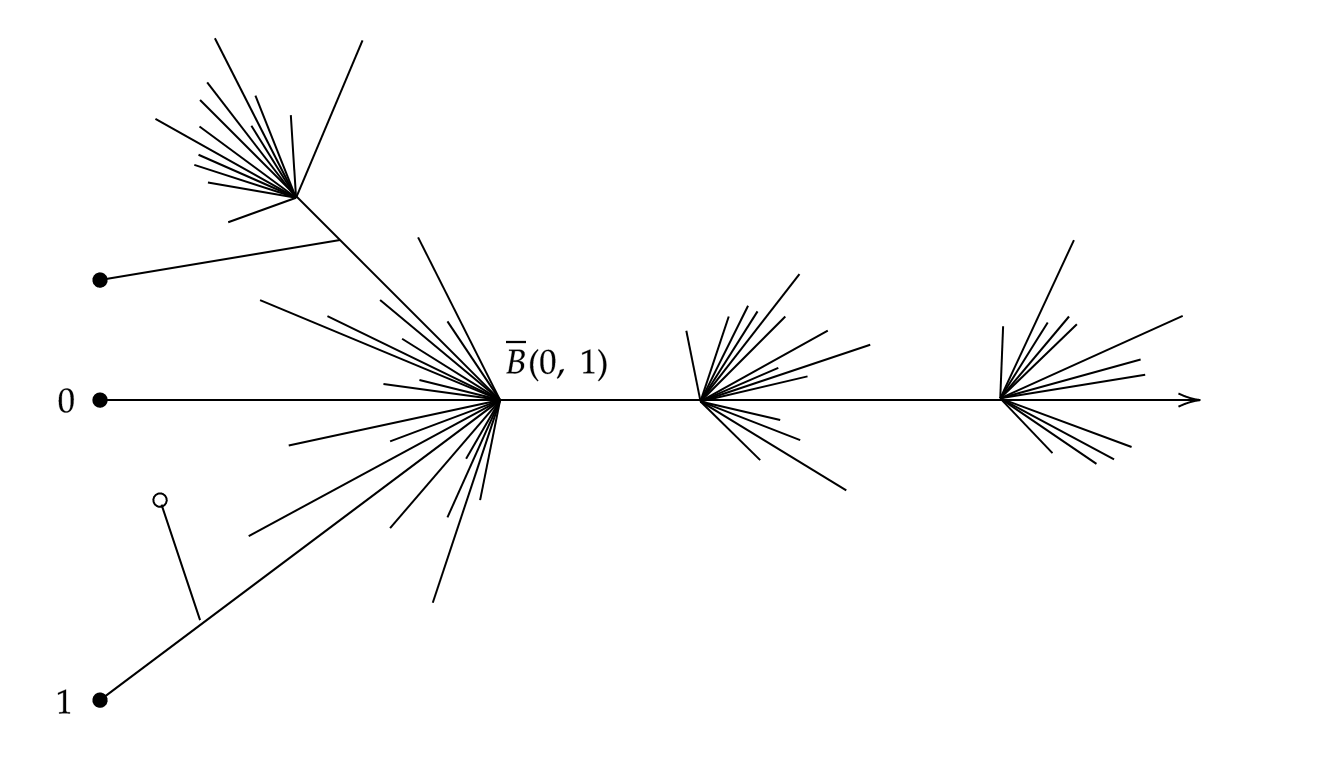
\includegraphics[width=0.7\textwidth]{Images/affineline.png}
    \caption{Visualisation of $\affline$}
    \label{fig:affline}
\end{figure}

Following the presentation in \parencite{bpr}, we now define some analytic domains in $\affline$ by using the fact that there is a continuous map $\sigma: \RR_{\geq 0} \to \affline$ mapping $r \mapsto \zeta_{0, r}$, which is a homeomorphism onto its image. 
We will refer to this image as the embedded real line. 
Then, $\sigma$ is a section of the map $\evt(x) = |T|_x$, and we find that these maps make the embedded real line into a strong deformation retract of $\affline$. 
Indeed, for any point $x \in \affline$, there is a point $\alpha := \sigma \circ \evt(x)$ lying on the embedded real line. 
By our earlier exposition, there is then a path $\gamma$ from $x$ to $\alpha$ parameterised by the unit interval. 
Hence, the map $F(x, t) = \gamma(t)$ is a homotopy satisfying the conditions of a strong deformation retract. 
These ideas will lead to the notion of the \textit{skeleton}, which will later become central to our study of $k$-analytic spaces.


We find that for any $I \subset \RR_{\geq 0}$, $\evt^{-1}(I)$ consists of the points which retract onto the points $\sigma(I)$. Then \cref{prop:diskmaxpoint} indicates that the closed (respectively, open) disk of radius $r \in |k^\times|$ can be visualised as $\evt^{-1}(I_r)$ where $I_r = [0, r]$ (respectively, $I_r = [0, r)$). Similarly, \parencite[\S 2.1]{bpr} we define the standard closed annulus $\mathbb{S}(a, b)$ of inner radius $|a|$ and outer radius $|b|$, for $0 < |a| \leq |b|$ and $a, b \in |k^{\times}|$ as the subset $\evt^{-1}([a, b])$, and when $a \neq b$, the standard open annulus as $\evt^{-1}((a, b))$. 
The closed annulus is affinoid, as it is identified with the spectrum of the following $k$-affinoid algebra:
\begin{align*}
k\{|a| \cdot T^{-1}, |b|^{-1} \cdot T\} & = \left\{ \sum_{i = -\infty}^{\infty} a_i T^i \; | \; |a_i| \cdot |a|^i \to 0 \; \text{as} \; i \to \infty, |a_i| \cdot |b|^i \to 0 \; \text{as} \; i \to -\infty \right\}.
\end{align*}

The norm on this algebra is given by 
\[
    \left\vert \sum_{n = -\infty}^{\infty} a_n T^n \right\vert = \max \{ |a_n| \cdot |a|^n, |a_n| \cdot |b|^n \}.
\]


\begin{figure}[!ht]
    \centering
    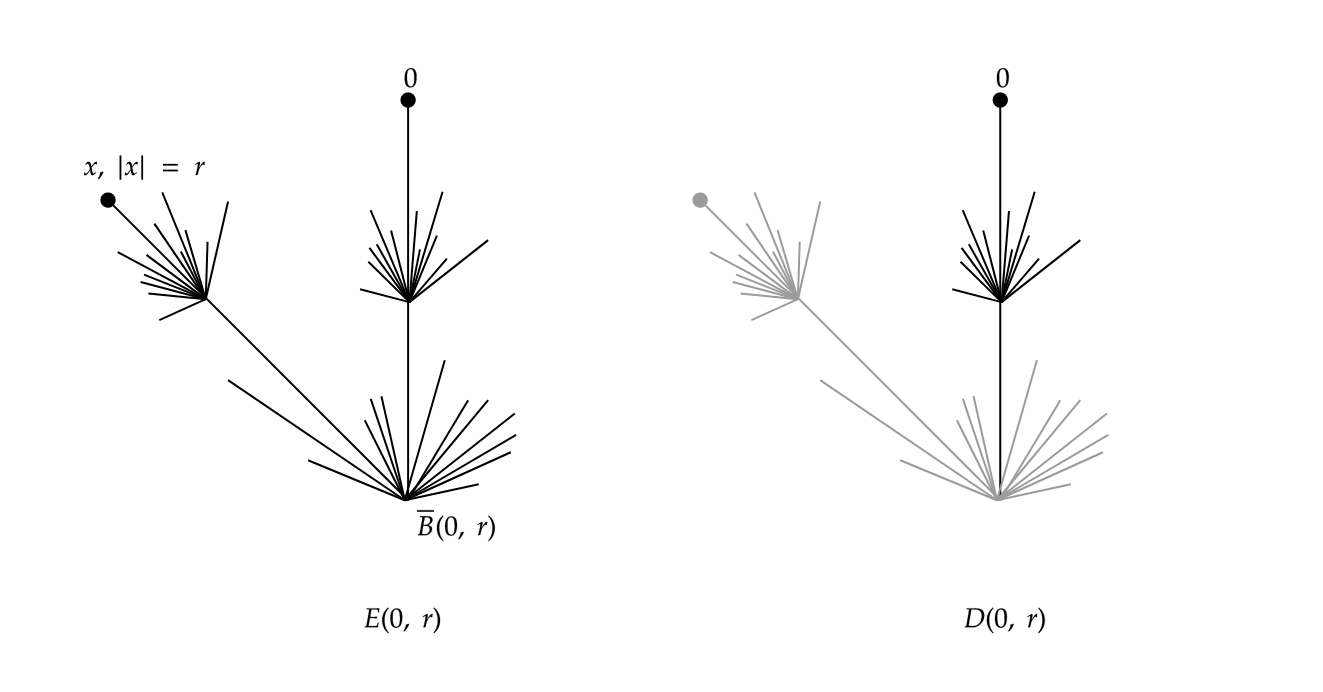
\includegraphics[width=0.8\textwidth]{Images/disks.png}
    \caption{Closed (left) and open (right) Berkovich disks}
    \label{fig:disks}
\end{figure}

\subsection{Gluing $k$-Analytic Spaces}

As is the case for topological and algebraic spaces, we may glue $k$-analytic spaces under appropriate conditions. A family of $k$-analytic spaces $\{X_i\}_{i \in I}$ gives gluing data if for each pair $i, j \in I$ there are analytic domains $X_{ij} \subset X_i, X_{ji} \subset X_j$ with an isomorphism $\mu_{ij}: X_{ij} \to X_{ji}$ satisfying the conditions:
\begin{enumerate}
    \item $X_{ii} = X_i$ and $\mu_{ii} = id$;
    \item $\mu_{ij}(X_{ij} \cap X_{ik}) = X_{ji} \cap X_{jk}$;
    \item $\mu_{ik} = \mu_{jk} \circ \mu_{ik}$.
\end{enumerate}

\begin{theorem} \label{gluing} \parencite[Prop. 1.3.3]{berk93}
    Let $\{X_i\}_{i \in I}$ be $k$-analytic gluing data. Suppose that one of the two following conditions holds.
    \begin{enumerate}
        \item Each $X_{ij} \subset X_i$ is open.
        \item Each $X_{ij} \subset X_i$ is closed, and for each $i \in I$, $X_{ij} \neq \emptyset$ for only finitely many $j \in I$.
    \end{enumerate}
    In each case, there exists a $k$-analytic space $X$ such that:
    \begin{enumerate}
        \item For each $i \in I$ there exists a morphism $\phi_i: X_i \to X$ making $X_i$ into an analytic domain in $X$.
        \item The images $\phi_i(X_i)$ cover $X$.
        \item $\phi_i(X_{ij}) = \phi_i(X_i) \cap \phi_j(X_j)$.
        \item $\phi_i(X_{ij}) = (\phi_j \circ \mu_{ij})(X_{ij})$
    \end{enumerate}
\end{theorem}

The proof of this is omitted and may be found in \textit{loc. cit.} Instead, we consider the analytic projective line to exemplify both types of gluing \parencite[Exercise 4.1.4.2]{temk}. 
Using the first kind of gluing, we may form $\projlinean$ using affine opens. Let $X_1 = X_2 = \affline$ and $X_{12} = X_{21} = {\{ x \in \affline \; | \; |T|_x \neq 0 \}}$. An isomorphism of analytic domains is then induced by the map $T \mapsto T^{-1}$. Concretely, it maps a seminorm $\snormx$ to the seminorm $|\cdot|_{1/x}$, where:
\[
    |a_nT^n + \cdots a_0|_{1/x} := |T|_{x}^{-n} \cdot |a_n + \cdots + a_0T^n|_x
\]
Using the second kind of gluing, $\projlinean$ may instead be constructed by gluing the unit disks $X_1 = X_2 = \berkspec{k\{T\}}$ along the closed analytic domains $X_{12} = X_{21} = {\berkspec{k\{T, T^{-1}\}}} = \{ x \; | \; |T|_x = 1 \}$. 
Similarly to the previous case, the isomorphism is induced by the homomorphism $k\{T, T^{-1}\} \to k\{T, T^{-1}\}$ mapping $T \mapsto T^{-1}$. 
This construction mirrors that of forming the Riemann sphere by gluing two closed disks along their boundaries. We will delay the proof that these two constructions are isomorphic until we have covered the notion of formal models; instead, we provide some pictorial intuition in \cref{fig:projline}. 
The left image visualises the gluing of the two affine lines while the right image shows the gluing of the unit disks; the analytic domains which are identified by the gluing are indicated with dashed lines.

\begin{figure}[!ht]
    \centering
    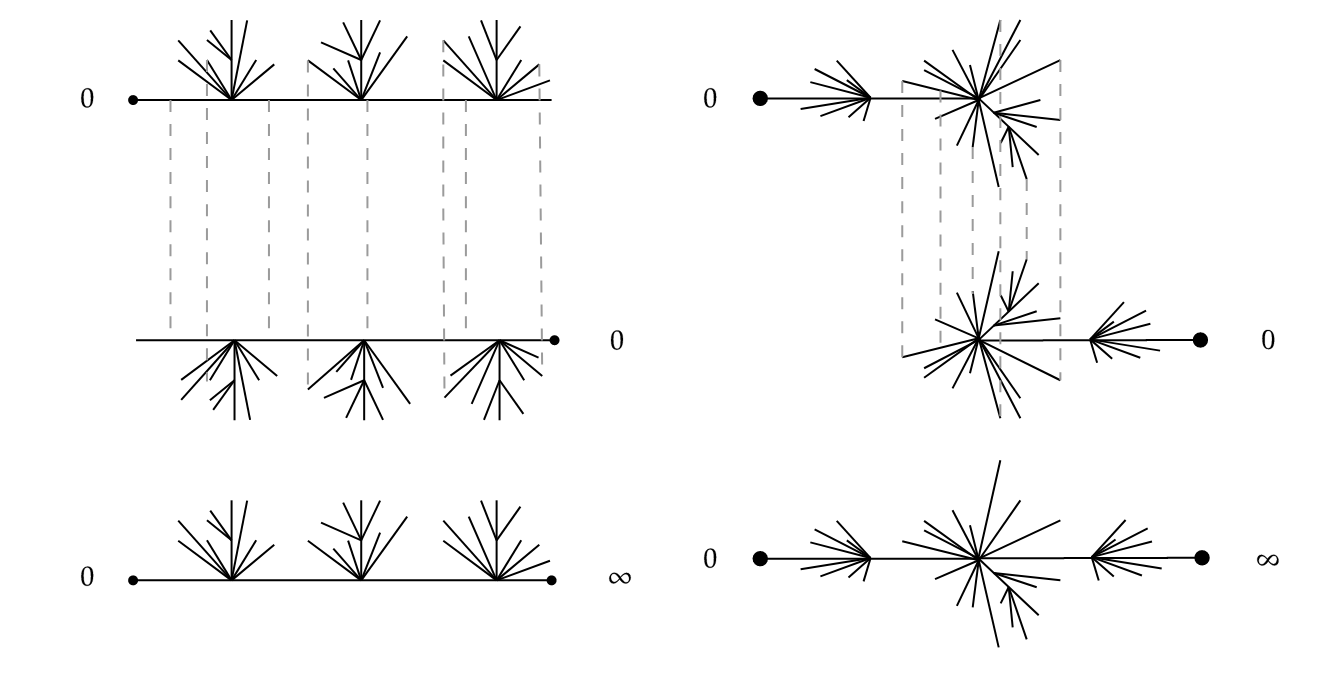
\includegraphics[width=0.8\textwidth]{Images/projspace.png}
    \caption{Two possible methods of constructing $\projlinean$}
    \label{fig:projline}
\end{figure}

The gluing procedure we have described may not, in general, result in a good $k$-analytic space.
For example, gluing two copies of the unit disk $\berkspeck{T}$ along the isomorphism given by $\berkspeck{T, T^{-1}} \cong \berkspeck{T, T^{-1}}$ given by the identity map.
In this case, we obtain the closed unit disk with a `doubled open unit disk.'
The point corresponding to $\zeta_{0, 1}$ does not admit an affinoid neighbourhood in this space.

\subsection{The Analytification Functor}

Similarly to the analytification of a complex variety, we can form the analytification of a variety over the non-Archimedean field $k$. The process is described following the presentation in \parencite[\S 3.4]{berk1}. The aim of the procedure is to assign to any scheme locally of finite type $X$ a $k$-analytic space $\anl{X}$ and a map $\iota: \anl{X} \to X$ of locally ringed spaces with the following universal property: if $Z$ is any $k$-analytic space and $\phi: Z \to X$ is a map of locally ringed spaces, then there is a unique factorization $\tilde{\phi}: Z \to \anl{X}$ through $\iota$, where $\tilde{\phi}$ is a map of $k$-analytic spaces.

For the scheme $\spec k[T_1, \dots, T_n]$, the analytification is the space $\mathbb{A}^{n, \text{an}}_{k}$ described previously. The map $\iota: \affnspace \to \mathbb{A}^{n}_{k}$ is given by mapping a seminorm to the point corresponding to the prime ideal given by its kernel.
Now assume we have obtained the analytification of $X$ and $Y \subset X$ is an open subscheme. Then we set $\anl{Y} = \iota^{-1}(Y) \subset \anl{X}$. 
If $Y \subset X$ is a closed subscheme defined by a coherent $\sheaf_{X}$ ideal $\mathfrak{J}$, then $\anl{Y}$ is the closed subspace cut out by $\mathfrak{J}\sheaf_{\anl X}$, which is a coherent $\sheaf_{\anl X}$ ideal. 
Finally, for any scheme $X$ locally of finite type covered by open affine subschemes $\{X_i\}_{i \in I}$, we may glue together the analytifications $X_i$ since by the universal property, the gluing data of the schemes induces gluing data for the analytifications. 
The canonical map of locally ringed spaces $\iota: \anl{X} \to X$ has the property that the induced homomorphism of stalks $\iota_x: \sheaf_{X, \pi(x)} \to \sheaf_{\anl{X}, x}$ is local and flat \parencite[Theorem 3.4.1]{berk1}. The proof that the constructions satisfy the desired universal property is omitted.

To exemplify the analytification functor, we now work out some explicit examples. Firstly, we note that the above construction applied to $\mathbb{P}^{1}_{k}$ yields the space $\projlinean$ constructed as the gluing of two analytic affine lines, justifying the notation.

Next, let $X$ be $n$-dimensional affine space and let $Y$ be the closed subscheme cut out by the ideal generated by some function $f \in k[T_1, \dots, T_n]$. Denote the corresponding $\sheaf_{X}$-ideal by $\mathfrak{J}$ and the $\sheaf_{\anl X}$-ideal corresponding to $\anl Y$ by $\anl{\mathfrak{J}}$. The space $\anl{Y}$ is identified, by construction, with the set of points 
\[
\{ x \in \mathbb{A}^{n, \text{an}}_{k} \; \vert \; \forall g \in \anl{\mathfrak{J}_{x}}, \; \; g(x) = 0 \}
\] 
where $g(x)$ denotes the image of $g$ in the residue field $\kappa(x) := \sheaf_{\mathbb{A}^{n, \text{an}}, x}/\mathfrak{m}_{x}$. Hence, it may be described as the points $x$ where $\anl{\mathfrak{J}_{x}} \subset \mathfrak{m}_{x}$. Denoting by $f_x := \pi_{x}(f_{\pi(x)})$ the image of the germ of $f$ at $\pi(x)$ under $\pi_x$ we find:
\[
\anl{\mathfrak{J}_x} \subset \mathfrak{m}_x
\iff \mathfrak{J}_{\pi(x)} \sheaf_{\anl X, x} \subset \mathfrak{m}_{\anl X, x} 
\iff f_x \in \mathfrak{m}_{\anl X, x}  
\]
Now, since $\pi_x$ is local:
\begin{align*}
    f_x \in \mathfrak{m}_{\anl X, x}
    \iff f_{\pi(x)} \in \mathfrak{m}_{X, \pi(x)}
    \iff f(x) = 0 \in \resfield 
    \iff |f|_x = 0
\end{align*}
Therefore, $\anl Y$ is the set of points of $\anl X = \mathbb{A}^{n, \text{an}}$ that one might intuitively expect - namely, the seminorms $|\cdot|_x$ on $k[T_1, \dots, T_n]$ such that $|f|_x = 0$.

Another example which will appear often is the analytification of the algebraic torus. As a scheme, we have that $\mathbb{G}_{m, k} = \spec k[T, T^{-1}]$, which is an open subscheme of the affine line. Hence, the analytification is given by the set of points $x \in \affline$ such that the kernel is not the ideal $(T)$, so $\anl{\mathbb{G}_{m, k}} \subset \affline$ consists of every point except for the type I point $\zeta_{0, 0}$.

The analytification preserves several desirable properties, which we state without proof (see \parencite[Theorem 3.4.8]{berk1}).
We will use these facts freely in the sequel.
Let $X$ be a scheme of locally finite type over $k$. 
Then:
\begin{enumerate}
    \item $X$ is separated if and only if $\anl{X}$ is Hausdorff;
    \item $X$ is proper if and only if $\anl{X}$ is Hausdorff and compact;
    \item $X$ is connected if and only if $\anl{X}$ is arcwise connected;
    \item the dimension of $X$ equals the topological dimension of $\anl{X}$.
\end{enumerate}

The full theory of Berkovich spaces is a deep and rich field of study of which we have seen only a small glimpse.
Equipped with our understanding of analytic spaces, we now broaden our investigations from the affine line to more general analytic curves.


\chapter{$k$-Analytic Curves}

In this chapter, we aim to further develop intuition surrounding the structure of analytic spaces.
Whereas giving an explicit picture for higher dimensional $k$-analytic spaces is difficult, curves have the advantages that they yield visualisations as in the case of the affine line.
The theory of $k$-analytic curves is a rich field of study, and presently we will focus on studying curves and their \textit{skeleta} through formal models.

\section{Generic Fibers of Formal Schemes}

We first give an overview of the theory of formal schemes, following \parencite[Chapter~7]{boschformal}.
Recall that a topological ring $A$ is said to have an $\mathfrak{a}$-adic topology, where $\mathfrak{a}$ is an ideal of $A$, if the subsets $\mathfrak{a}^n$ form a basis of neighbourhoods of $0$.
The $\mathfrak{a}$-adic completion for such a ring is defined as $\hat{A} = \varprojlim_{n} A/\mathfrak{a}^n$; the resulting ring is Hausdorff and complete.
Where $\mathfrak{b}$ is an ideal such that $\mathfrak{a}^n \subset \mathfrak{b}$ and $\mathfrak{b}^n \subset \mathfrak{a}$ for some $n$, then the topologies generated by the two ideals are equivalent, and any such ideal $\mathfrak{b}$ is known as an ideal of definition of $A$.

Now assume $A$ is a complete and Hausdorff $\mathfrak{a}$-adic ring.
Similarly to the $\operatorname{Spec}$ construction, the affine building blocks are given by $\spf A$, the formal spectrum. As a topological space, $\operatorname{Spf} A$ is given by
the underlying topological space of $\spec A/\mathfrak{a}$ and hence, it consists of open prime ideals of $A$.
We endow $\spf{A}$ with a structure sheaf $\sheaf_{\spf{A}}$ where for each open $U \subset \spf{A}$, we define 
\[
    \sheaf_{\spf{A}}(U) = \varprojlim \sheaf_{\spec{A/\mathfrak{a}^n}}(U)
\]
where the inverse limit is taken in the category of topological rings, and the topology on each $\sheaf_{\spec{A/\mathfrak{a}^n}}(U)$ is discrete.
The right hand side of the expression is well defined, since for all $n > 0$, the immersion $\spec A/\mathfrak{a}^n \to \spec{A/\mathfrak{a}}$ is a homeomorphism.
Generally, a formal scheme is then a locally topologically ringed space where each point has an open neighbourhood isomorphic to an affine formal scheme.
Morphisms of formal schemes are morphisms in the category of locally topologically ringed spaces.

We are interested particularly in a certain class of formal schemes, of which we now give an overview following \parencite[\S 5.2.1]{temk}.
Fix a non-zero element $\pi$ of the maximal ideal of $R$, which is then a $\pi$-adic ring.
Let $R\{T_1, \dots, T_n\}$ be the algebra given by $k\{T_1, \dots, T_n\} \cap R[[T_1, \dots, T_n]]$.
Hence, it consists of formal power series over $R$ in $n$ variables which converge on the closed unit disc.
We say an $R$-algebra $A$ is of \textit{topologically finite presentation} (tfp) if it is isomorphic to the algebra $R\{T_1, \dots, T_m\}/I$, for some finitely generated ideal ideal $I$.
In addition, $A$ is called \textit{admissible} if it is tfp and it does not have $\pi$-torsion.
If $A$ is tfp, then it can be shown that $A \otimes_{R} k$ is a $k$-affinoid algebra admitting an admissible epimorphism $k\{T_1, \dots, T_n\} \to A \otimes_{R} k$, for some $n$.
We will say that a formal $R$-scheme $\fmodel$ is locally finitely presented (lfp), resp. admissible, if $\fmodel$ has a locally finite cover by open affine formal schemes of the form $\spf A$, where $A$ is tfp, resp. admissible.

Let $X$ be a $R$-scheme with a locally finite covering by open subschemes $\spec A$, where each $A$ is finitely presented as a $R$-algebra.
Then, we can define the formal completion $\hat{X}$ as follows. 
Let $\mathfrak{J}$ be the quasi-coherent ideal sheaf generated by $\pi$.
Then, $\hat{X}$ is defined as a topological space to be the topological space underlying the closed subscheme $Y$ of $X$ cut out by $\mathfrak{J}$, with the sheaf of topological rings $\sheaf_{\hat{X}} = \varprojlim \sheaf_{X}/\mathfrak{J}^{n}$, where each sheaf $\sheaf_{X}/\mathfrak{J}^{n}$ is restricted to $Y$ along the inclusion $Y \to X$.
Locally, let $X = \spec A$; then $\hat{X}$ is given by $\spf{\hat{A}}$, where $\hat{A}$ is the completion of $A$ with respect to the ideal $\pi A$.

For a lfp formal scheme $\fmodel$, we define its \textit{special fiber} $\fmodel_s := \fmodel \times_{R} \tilde{k}$, where the fiber product is taken in the category of formal schemes.
Then, $\fmodel_s$ is a scheme locally of finite presentation over $\tilde{k}$. 
Locally, the special fiber of $\fmodel = \spf{A}$ is given by the scheme $\spec{A/\maxideal A}$.

Furthermore, we assign to an lfp formal scheme $\fmodel$ a $k$-analytic space $\fmodel_{\eta}$, known as the generic fiber of $\fmodel$.
Firstly, if $\fmodel = \spf A$, then we set $\fmodel_{\eta} = \berkspec{A \otimes_{R} k}$.
A map $\spf A \to \spf B$ corresponds to a continuous homomorphism $B \to A$, which induces a homomorphism of $k$-affinoid algebras $B \otimes_{R} k \to A \otimes_{R} k$ and hence of $\berkspec{A \otimes_{R} k} \to \berkspec{B \otimes_{R} k}$.

Next, assume $\fmodel$ is separated and choose a locally finite covering by open affine formal subschemes $\{ \fmodel_{i} \}_{i \in I}$.
Then, each intersection $\fmodel_{ij} = \fmodel_i \cap \fmodel_j$ is also an affine open formal subscheme.
It is a fact that if $\mathfrak{Y} \to \fmodel$ is an open immersion of affine formal schemes, then $\mathfrak{Y}_{\eta} \to \fmodel_\eta$ is the embedding of an affinoid domain.
Hence, we may glue the affinoid spaces $\{ (\fmodel_{i})_{\eta} \}_{i \in I}$ along the affinoid domains $\{ (\fmodel_{ij})_{\eta} \}_{i, j \in I}$ using \cref{gluing}.
A morphism $\mathfrak{Y} \to \fmodel$ of separated formal schemes induces a morphism $\mathfrak{Y}_{\eta} \to \fmodel_\eta$ by gluing the induced morphisms $(\mathfrak{Y}_i)_{\eta} \to \fmodel$, where $\{\mathfrak{Y}_i\}$ is a locally finite covering by open affine formal subschemes.

If $\fmodel$ is arbitrary with a covering $\{ \fmodel_i \}_{i \in I}$ by separated formal schemes, then the intersections $\fmodel_{ij}$ are separated formal schemes, and it can be shown that $(\fmodel_{ij})_{\eta}$ is a compact analytic domain in $(\fmodel_i)_{\eta}$ and $(\fmodel_j)_{\eta}$.
We may therefore glue $(\fmodel_i)_{\eta}$ and $(\fmodel_j)_{\eta}$ along $(\fmodel_{ij})_{\eta}$ as before to obtain $\fmodel_{\eta}$.
Since affinoid and compact analytic domains are closed subsets in a Hausdorff space, the fact that the cover is locally finite is necessary to perform the gluing.
Similarly to the separated case, we may also define a morphism of $k$-analytic spaces $\mathfrak{Y}_{\eta} \to \mathfrak{X}_{\eta}$ for any morphism $\mathfrak{Y} \to \mathfrak{X}$ by gluing appropriately.
It may then be verified that $\eta$ gives a functor, known as the generic fiber functor.

There is a canonical reduction map $\operatorname{red}_{\fmodel}: \fmodel_\eta \to \fmodel_s$ which is defined by the following procedure. 
Let $x \in \fmodel_\eta$ be a point and $\spf{A} \subset \fmodel$ such that $(\spf{A})_\eta$ contains $x$.
Then $x$ defines a character $A \otimes_{R} k \to \resfield$ and hence a homomorphism $A \to A \otimes_{R} k \to \resfield$.
The following lemma shows that the image of this map lands inside $\resfield^{\circ}$.

\begin{lemma}\label{lemma:ringfactors} \parencite[Exercise 5.2.2.6]{temk}
    Suppose $A$ is a tfp $R$-algebra, generated by $f_1, \dots, f_n$.
    Then for all $x \in (\spf{A})_{\eta}$ and $1 \leq i \leq n$ we have $|f_i|_x \leq 1$.
\end{lemma}
\begin{proof}
    We may find an admissible epimorphism $\phi: k\{T_1, \dots, T_n\} \to A \otimes_{R} k$ such that $T_i \mapsto f_i$ for each $i$.
    Denote $\mathbb{B}^{n} = \berkspeck{t_1, \dots, t_n}$.
    Then the morphism $\phi$ induces a map $\phi^{*}: \berkspec{A \otimes_{R} k} \to \mathbb{B}^n$, where a point $x \in \berkspec{A \otimes_{R} k}$ gives a point $\phi^{*}(x) \in \mathbb{B}^n$ by the equation $|f|_{\phi^{*}(x)} = |\phi(f)|_x$.
    Hence, we see that $|f_i|_x = |\phi(t_i)|_x = |t_i|_{\phi^{*}(x)} \leq 1$, where the final inequality follows from the fact that the norm $||\cdot||$ on $k\{t_1, \dots, t_n\}$ is such that $||t_i|| = 1$, and any element of the Berkovich spectrum is bounded by this norm.
\end{proof}

\Cref{lemma:ringfactors} shows that $x \in (\spf A)_{\eta}$ induces a map $A \to \resfield^{\circ}$ where the image of the ideal $\pi A$ lands in $\resfield^{\circ \circ}$.
Hence, there is a well-defined map $A/\pi A \to \resresfield$.
Then, $\red{\fmodel}{x}$ is defined to be the point given by $\spec \resresfield \to \fmodel_s$.
This map is anti-continuous, in that the inverse image of an open (resp. closed) set is closed (resp. open).

If $X$ is an $R$-scheme locally of finite presentation, there are now two ways to obtain a $k$-analytic space: either by taking the generic fiber of the formal completion $\hat{X}_{\eta}$ or by taking the analytification of the generic fiber $\anl{X_k}$, where $X_k := X \times_{R} k$.
In general, there is a canonical map $\i_{X}: \hat{X}_{\eta} \to \anl{X_{k}}$, which we can construct as follows \parencite[\S 5.3]{bconrad}.
By the universal property of analytification, it suffices to give a map of locally ringed spaces $\hat{X}_{\eta} \to X_{k}$. Consider the case where $X = \spec A$ is affine, for some finitely generated $R$-algebra $A$.
There is a canonical map $A \otimes k \to \hat{A} \otimes k$ and it is a standard result that $\operatorname{Hom}(Y, X) \cong \operatorname{Hom}(\Gamma(X, \sheaf_X), \Gamma(Y, \sheaf_Y))$ for a locally ringed space $Y$ and an affine scheme $X$ \parencite[Tag 01I1]{stacks-project}. 
Hence, we immediately obtain a map $\hat{X}_{\eta} \to X_k$, which gives the desired morphism $i_X: \hat{X}_{\eta} \to \anl{X_k}$.
This morphism is `functorial' in the following sense: if $X \to Y$ is a morphism of affine schemes, then we have an induced commuting square \footnote{This may be more formally stated by saying that $i_X$ is a functor from the category of affine schemes to the arrow category of $k$-analytic spaces.}:
\[
\begin{tikzcd}
 & \hat{X}_{\eta} \arrow[r] \arrow[d] & \anl{X_k} \arrow[d] \\
 & \hat{Y}_{\eta} \arrow[r] & \anl{Y_k}
\end{tikzcd}
\]
This follows from the fact that for any morphism $A \to B$ of finitely presented $R$-algebras, the following square commutes.
\[
\begin{tikzcd}
 & A \otimes k \arrow[r] \arrow[d] & \hat{A} \otimes k \arrow[d] \\
 & B \otimes k \arrow[r] & \hat{B} \otimes k
\end{tikzcd}
\]



As in the case of constructing the generic fiber functor, we may extend this map first to the case where $\hat{X}$ is a separated formal scheme, and then to the case where $\hat{X}$ is non-separated, to obtain a functorial canonical morphism $i_X$ for any scheme $X$ locally of finite presentation over $R$.

\begin{example}
    Let $X = \mathbb{A}^{1}_{R}$. Then we find that $\anl{X_k} = \affline$, while $\hat{X}_{\eta} = \berkspec{k\{t\}}$ is the unit disk. 
    In this case, $i_X : \berkspec{k\{t\}} \xhookrightarrow{} \affline$ is the canonical embedding of the closed unit disk into the affine line.
\end{example}

\begin{example}
    Let $X$ be the affine line over $R$ with doubled origin. 
    As a scheme, this is formed by gluing the affines $\spec R[T]$ and $\spec R[S]$ by identifying the opens $\spec R[T, T^{-1}], \spec R[S, S^{-1}]$ using the isomorphism $T \mapsto S$. The space $X_k$ is then the analytic affine line with doubled origin. 
    However, the generic fiber of the formal completion of $X$ is a little more interesting: it is in fact the closed unit disk with doubled open unit disk which we previously encountered as an example of a generalized space which is not good space.
    The map $i_X$ then identifies $\hat{X}_{\eta}$ with the closed unit disk in the affine line with doubled origin.
    Except for the origin, each point lying on an open unit disk and its copy are both identified with the same point in $\anl{X}_k$.
    Hence, $i_X$ is not injective.
\end{example}

The following lemmas and theorems, adapted from \parencite[Exercise 5.2.3.1]{temk} describe the map $i_X$ more generally. 
The details of these facts are often omitted in the literature, so we provide some proofs.

\begin{lemma}\label{lemma:affinecaseisaffinoid}
    If $X$ is an affine scheme of finite presentation, then $i_X$ is the embedding of an affinoid domain.
\end{lemma}
\begin{proof}
    Let $X = \spec A$.
    Suppose $A$ is generated by $f_1, \dots, f_n$.
    Then, we may fix an admissible epimorphism $k\{T_1, \dots, T_n\} \to \hat{A} \otimes_{R} k$ mapping $T_i \mapsto f_i$.
    By \parencite[Corollary 2.3.2]{berk1}, the induced map \[\hat{X}_{\eta} = \berkspec{\hat{A} \otimes_{R} k} \to \mathbb{B}^{n} = \berkspeck{T_1, \dots, T_n}\] is a closed immersion, that is, it is the embedding of an analytic domain with closed image.

    The functoriality of $i_X$ then induces the following commuting diagram:
    \[
    \begin{tikzcd}
        \hat{X}_{\eta} \arrow[d] \arrow[r,"i_X"]  & \anl{X_k} \arrow[d] \\
        \mathbb{B}^n \arrow[r] & \mathbb{A}^{n, \operatorname{an}}_{k}
    \end{tikzcd}
    \]
    where the vertical and bottom maps are closed immersions of $k$-analytic spaces.
    Since the vertical and bottom maps are injective, it follows that $i_X$ is also injective.
    Since the source is compact and the target is Hausdorff, $i_X$ is a homeomorphism onto its image.
    Now let $Z \to \anl {X_k}$ be a morphism of $k$-analytic spaces such that the image is contained in $\hat{X}_{\eta} \subset \anl X$.
    It follows that there is an induced map $Z \to \affnspace$ with the image contained in $\mathbb{B}^{n} = \berkspec{k\{T_1, \dots, T_n\}}$, hence there is a induced map $Z \to \mathbb{B}^{n}$ since $\mathbb{B}^{n}$ is an affinoid domain in $\affnspace$.
    Furthermore, the map $Z \to \mathbb{B}^{n}$ has image contained in $\hat{X}_{\eta}$, so since $\hat{X}_{\eta}$ is an analytic domain in $\mathbb{B}^{n}$, we conclude that there is a map $Z \to \hat{X}_{\eta}$.
    Since each induced map was uniquely determined by the map $Z \to \anl X$, it follows that the map $Z \to \hat{X}_{\eta}$ is unique, so that $i_X: \hat{X}_{\eta} \to \anl X$ is the embedding of an affinoid domain.
\end{proof}

\begin{lemma}\label{lemma:genericfibercharacterization}
    The points $y \in \hat{X}_{\eta}$ are in bijection with the set of maps $\spec{\resfieldof{x}^\circ} \to X$ extending the map $\spec{\resfieldof{x}} \to X$, where $x = i_X(y)$.
\end{lemma}
\begin{proof}
    Fix a point $y \in \hat{X}_{\eta}$ and let $i_X(y) = x$. 
    Now let $\spec A$ be an affine open in $X$ such that $y \in (\spf{\hat{A}})_{\eta}$, from which it follows that $i_X(y) = x \in \anl{(\spec A_k)}$.
    By \cref{lemma:affinecaseisaffinoid}, the restriction of $i_X$ to $(\spf{\hat{A}})_{\eta}$ is the embedding of an affinoid domain into $\anl{(\spec{A_k})}$; since the completed residue field may be computed within an affinoid domain containing the point, it follows that $\resfieldof{y} \cong \resfield$. 
    
    Next, we consider the map 
    \[A \to \hat{A} \otimes_{R} k \to \resfieldof{y} \cong \resfieldof{x}.\]
    The image of $A$ along this map lands in $\resfieldof{y}^\circ \cong \resfield^\circ$ by lemma~\ref{lemma:ringfactors}, so that there is a factorisation $A \to \resfieldof{x}^{\circ}$.
    This gives a lift $\spec{\resfield^\circ} \to \spec{A} \xhookrightarrow{} X$.
    
    Conversely, suppose that such a lift exists. Then, the image of $\spec{\resfield^\circ} \to X$ is contained within some affine open $\spec A$, since $\resfield^\circ$ is local. 
    Hence, we have a homomorphism $A \to \resfield^\circ$, which, by passing to completions, determines a homomorphism $\hat{A} \to \resfield^{\circ}$ and subsequently a map $\hat{A} \otimes_{R} k \to \resfield$. 
    This is a character corresponding to some point $y \in (\spf{\hat{A} \otimes_{R} k})_\eta \xhookrightarrow{} \hat{X}_\eta$. Since the map $\spec{\resfield^\circ} \to X$ extends the map $\spec{\resfield} \to X$, it follows by construction of $i_X$ that $i_X(y) = x$.
    
    The two procedures are verified to be inverses of each other.
\end{proof}

\begin{theorem}\label{separatedix}
If $X$ is separated and quasi-compact then the map $i_X$ is the embedding of a compact analytic domain.
\end{theorem}
\begin{proof}
The valuative criterion of separatedness indicates that there exists at most one lift $\spec{\resfield^{\circ}} \to X$ of a map $\spec{\resfield} \to X$. 
Hence, by \cref{lemma:genericfibercharacterization}, $i_X$ is injective. 
The source is compact since it is a finite union of affinoid domains which are compact and the target is Hausdorff, hence, it must be a homeomorphism onto its image.
At each point $y \in \hat{X}_{\eta}$ there exists an affinoid neighbourhood $V$ of $y$ in $\hat{X}_{\eta}$ such that the restriction of $i_X$ to $V$ is the embedding of an affinoid domain $V \to \anl{X}$, hence $i_X(\hat{X}_{\eta}) \subset \anl X$ is such that each point has an affinoid neighbourhood in $i_X(\hat{X}_{\eta})$.
It follows that $i_X$ is the embedding of an analytic domain.
\end{proof}

\begin{corollary} \label{properisiso}
If $X$ is proper over $R$, then there is an isomorphism $i_X: \hat{X}_\eta \xrightarrow{\sim} \anl{X_k}$.
\end{corollary}
\begin{proof}
The valuative criterion of properness indicates that there exists precisely one lift $\spec{\resfield^{\circ}} \to X$ of a map $\spec{\resfield} \to X$. 
By \cref{lemma:genericfibercharacterization}, it follows that $i_X$ is surjective, and since $X$ is necessarily separated, we find that $\hat{X}_\eta$ is an analytic domain in $\anl{X}_k$, so that $i_X$ is an isomorphism.
\end{proof}

Letting $X = \mathbb{P}^{1}_{R}$, we find that $\hat{X}_{\eta}$ is the gluing of two closed disks $\berkspec{k\{T\}}$ and $\berkspec{k\{S\}}$ along the isomorphism $\berkspec{k\{T, T^{-1}\}} \cong \berkspec{k\{S, S^{-1}\}}$ given by $T \mapsto S^{-1}$.
On the other hand, $\anl X$ is the gluing of two copies of $\affline$ along the isomorphism $\anl{\mathbb{G}_{m, k}} \cong \anl{\mathbb{G}_{m, k}}$ given by $T \mapsto T^{-1}$.
\Cref{properisiso} finally shows that the two constructions are isomorphic.

In this example, the formal scheme $\hat{X}$ can be considered as a \textit{formal model} for the $k$-analytic space $\anl{X}$.

\begin{defn}
    A formal $R$-model $\fmodel$ for a $k$-analytic space $X$ is an admissible formal $R$-scheme equipped with an isomorphism $\fmodel_{\eta} \cong X$.
\end{defn}

As we will see, models are spaces capturing the geometry of the $k$-analytic space in a (formal) scheme which is potentially easier to study.
If $X$ is a proper $k$-scheme locally of finite type, then $\anl{X}$ admits a formal model \parencite[Remark 5.3.3.2]{temk}.

\section{Skeleta of $k$-Analytic Curves}

\subsection{Classification of Points}

To begin, we must consider the notion of dimension, which is more subtle for $k$-analytic spaces than in the case of schemes.
An obstruction is the fact that for $k$-affinoid algebras, the Krull dimension is not preserved under extension of the base field.
An example of this, as found in \parencite[\S 3.5]{temk}, is the $k$-affinoid algebra $K_r := k\{r^{-1} T, rT^{-1}\}$.
For $r \not\in \sqrt{|k^{\times}|}$, $K_r$ is a field, and hence has Krull dimension $0$, but $K_r \hat{\otimes}_{k} K_r \cong K_r\{T\}$ does not.
This motivates the following definition.

\begin{defn} \parencite[\S 2.3]{berk1}.
    The dimension $\dim(X)$ of a $k$-affinoid space $X = \berkspec{\banr}$ is the Krull dimension of the algebra $\banr \hat{\otimes}_{k} K$, where $K$ is a non-Archimedean field extension of $k$ such that there exists an admissible epimorphism $K\{T_1, \dots, T_n\} \to \banr \hat{\otimes}_{k} K$.
\end{defn}

 It can be shown that such a field extension exists, and that $\dim(X)$ is independent of the choice of extension.
 We extend this notion to a general $k$-analytic space $X$, by defining its dimension $\dim(X)$ to be the supremum of the dimensions of the $k$-affinoid domains of $X$.
 
 Following \parencite{bpr}, we define a $k$-analytic curve to be the analytification of a smooth, proper, geometrically connected algebraic curve over $k$.
 We caution the reader that other sources map give more a general definition, which may require more theory to be built up, but our definition will capture all the cases we are interested in.
 It can be shown that such a space is of dimension one by invoking the appropriate GAGA theorems \parencite[Corollary 3.2.8]{berk1} \parencite[Proposition 3.4.3]{berk1}.

The classification of points for the affine line may then be extended to more general curves.
For each valued extension $k \subset K$, we associate the parameters:
\begin{align*}
    & E(K) = \dim_{\QQ}\left(|K^{\times}|/|k^{\times}| \otimes_{\ZZ} \QQ\right) \\
    & F(K) = \operatorname{tr.deg.}(\tilde{K} / \tilde{k}).
\end{align*}

Let $X$ be a $k$-analytic space of dimension $n$.
Fixing a point $x \in X$, we denote $E(x) := E(\resfield)$ and $F(x) := F(\resfield)$.
Then, it may be shown that $E(x) + F(x) \leq n$ \parencite[Lemma 2.5.2]{berk93}.
In the case where $n = 1$, we can then classify $x$ as follows \parencite[\S 2.3.3]{temk}:
\begin{enumerate}
    \item $x$ is type I if $\resfield \subset \widehat{k^a}$, where $\widehat{k^a}$ is the completed algebraic closure of $k$;
    \item $x$ is type II if $E(x) = 0$ and $F(x) = 1$; 
    \item $x$ is type III if $E(x) = 1$ and $F(x) = 0$;
    \item $x$ is type IV if $E(x) = F(x) = 0$ and $x$ is not of type I.
\end{enumerate}

Note that if $x$ is type I then $E(x) = F(x) = 0$.
It may be verified that this is an extension of our earlier classification of the points of the affine line over an algebraically closed field.

\subsection{Skeleta of Annuli}

For the rest of this chapter, we assume that $k$ is algebraically closed.

Recall that we defined maps $\evt: \affline \to \mathbb{R}_{\geq 0}$ and $\sigma: \mathbb{R}_{\geq 0} \to \affline$, where $\evt(x) = |T|_x$ and $\sigma(r) = \zeta_{0, r}$.
Using these maps, we were able to define several analytic domains in $\affline$, including \textit{standard open} and \textit{standard closed} annuli, denoted by $\annulus{a, b}_{+}$ and $\annulus{a, b}$ respectively, for some $a, b \in k^{\times}$ with $|a| \leq |b|$.
When $b = 1$, we will denote the annulus as $\annulus{a}$.
Denoting $c = ab^{-1}$, we have a series of isomorphisms:
\[\annulus{a, b} \cong \annulus{c} \cong \berkspec{k\{t, |c| \cdot t^{-1}\}} \cong \berkspec{k\{t, s\}/(st - c)}. \]
If $X$ is any $k$-analytic space which is isomorphic to a standard closed (resp. open) annulus, then we will call $X$ a \textit{generalized closed} (resp. \textit{generalized open}) annulus.
A standard annulus is any standard open or standard closed annulus, and a generalized annulus is any space which is either a generalized open or a generalized closed annulus.
Similarly, if $X$ is isomorphic to a standard closed (resp. open) ball, then $X$ will be called a \textit{generalized closed} (resp. \textit{generalized open}) ball.


Next, recall that we defined a strong deformation retraction from $\affline \to \sigma(\mathbb{R}_{\geq 0})$.
In order to obtain a suitable notion of a skeleton for an arbitrary curve, we make a similar definition for an annulus.

\begin{defn}\parencite[\S 2.3]{bpr}
    For any standard closed or open annulus $A$, its \textit{skeleton} is the subset \[\Sigma(A) := \sigma(\evt(A)). \]
\end{defn}

There is then a map $\rho_A := \sigma \circ \evt$ which is a retraction of $A$ onto $\Sigma(A)$, and can be shown to be a strong deformation retraction \parencite[Proposition 4.1.6]{berk1}.
If $X$ is a generalized annulus, then fixing an isomorphism $\phi: X \to A$ for some standard annulus $A$, then the skeleton $\Sigma(X)$ of $X$ is defined as $\phi^{-1}(\Sigma(A))$, and there is a corresponding retraction $\rho_X = \phi^{-1} \circ \rho_A \circ \phi$.
It can be shown that $\Sigma(X)$ and $\rho_X$ do not depend on $A$ or $\phi$ \parencite[Corollary 2.6]{bpr}.

The following lemma describes the retraction map.

\begin{lemma} \label{annulusretract} \parencite[Lemma 2.12]{bpr}
    Let $A$ be a generalized annulus. 
    Then $A \backslash \Sigma(A)$ is an analytic domain in $A$ isomorphic to an infinite disjoint union of open balls.
    If $\overline{B}$ is the topological closure of an open ball $B$ in the disjoint union, then $\overline{B} \backslash B = \{ x \}$, and for every point $y \in B$, we have $\rho_{A}(y) = x$.
\end{lemma}

Before giving the proof, we consider the standard closed annulus \[\annulus{1} = \berkspeck{t, t^{-1}} \cong \berkspec{k\{s, t\}/(s t - 1)}.\]
Then, the affine formal scheme $\fmodel = R\{s, t\}/(st - 1)$ is such that $\fmodel_{\eta} \cong \annulus{1}$, and hence $\fmodel$ is a formal $R$-model for $\annulus{1}$.
In this case, $\fmodel_s \cong \spec \tilde{k}[s, t]/(st - 1)$ is the affine open subscheme of the affine line over $\tilde{k}$ given by removing the origin, and we wish to describe $\operatorname{red}_{\fmodel}$ explicitly.
Firstly, consider the point $x = \zeta_{0, 1} \in \berkspeck{t, t^{-1}}$.
Then $\resresfield \cong \tilde{k}(t)$, and the map $\tilde{k}[t, t^{-1}] \to \tilde{k}(t)$ is the natural map.
The kernel of this map corresponds to the zero ideal, hence $\red{\fmodel}{x}$ is the generic point of $\fmodel_s$.
Next, assume that $x \in D(b, 1)$ for some $b \in R^{\times}$.
The claim is that $\red{\fmodel}{x}$ is the point given by the maximal ideal $(t - \tilde{b})$, where $\tilde{b}$ is the residue class of $b$ in $\tilde{k}$.
Indeed, we see that $|t - b|_x < 1$, so that $(t - \tilde{b}) \subset \ker (\tilde{k}[t, t^{-1}] \to \resresfield)$.
By maximality of $(t - \tilde{b})$ and the fact that the kernel of the map $\tilde{k}[t, t^{-1}] \to \resresfield$ is a prime ideal as $\resresfield$ is a field, it follows that the inclusion is an equality.

\begin{proof}[Proof of \cref{annulusretract}]
    We elaborate on the proof given in \textit{loc. cit.}
    If $A = \annulus{1}$, then the first two claims follow by the remarks preceding the proof and the fact that $\tilde{k}$ is infinite.
    The last statement is a consequence of the anti-continuity of $\operatorname{red}_{\fmodel}$.
    Indeed, let $B$ be an open ball as in the statement, so $\red{\fmodel}{b} = \{y \}$ for all $b \in B$, where $y$ is a closed point.
    If $z \in \overline{B}$, then $z$ is contained in any closed set containing $B$.
    Now let $U$ be any open in $\fmodel_s$ containing $y$; then $\operatorname{red}^{-1}_{\fmodel}(U)$ is a closed set and so it contains $z$.
    Therefore, $U$ contains $\red{\fmodel}{z}$.
    Since $U$ was arbitrary, it follows that $z \in \operatorname{red}^{-1}_{\fmodel}(\xi)$, where $\xi$ is the generic point of $\fmodel_s$.
    Hence, $z = \zeta_{0, 1}$.
    
    Next, assume $A$ is any generalized annulus, and by fixing an isomorphism, we may assume it is a standard annulus.
    Let $r \in \evt(A)$.
    If $r \not\in |k^{\times}|$, then we claim that $\evt^{-1}(r)$ is a single type III point $x$.
    Indeed, if $y$ is any point such that $|T|_y = r$, then for any $b \in k$ we have $|T - b|_y = \max \{ |T|_y, |b| \} = |T - b|_x$, so that $y = x$.
    Hence it suffices to consider when $r \in |k^{\times}|$. 
    In this case, we may rescale so that $r = 1$, in which case $\evt^{-1}(r) = \annulus{1}$.
    It then suffices to show that the connected components of $\annulus{1} \backslash \{ \zeta_{0, 1} \}$ are the connected components of $A \backslash \Sigma(A)$ since then we reduce to the previous case.
    This follows if $\annulus{1} \backslash \{ \zeta_{0, 1} \}$ is both open and closed in $A \backslash \Sigma(A)$.
    It is closed since $\annulus{1}$ is closed, and $\annulus{1} \backslash \{ \zeta_{0, 1} \} = \annulus{1} \cap (A \backslash \Sigma(A))$, and it is open since it is a union of open balls of the form $D(b, 1)$.
\end{proof}

\subsection{Semistable Vertex Sets and Semistable Reduction}

Assuming $X$ is a smooth proper connected algebraic curve over $k$, we now develop the theory of semistable vertex sets following \parencite[\S 3-4]{bpr}, which allow the notion of a skeleton of an annulus to be used to construct a skeleton for $\anl X$.

Note that in the case of an annulus $\mathbb{S}(a, b)$, the skeleton is determined completely by the type II points $\zeta_{0, |a|}$ and $\zeta_{0, |b|}$ which form the endpoints, since the skeleton is then the unique path between the two points.
Removing these two points results in a disjoint union of an open annulus $\mathbb{S}(a, b)_{+}$ and infinitely many open balls.
This observation motivates the following definitions.

\begin{defn} \parencite[Definition 3.1]{bpr}
    A semistable vertex set $V$ of $X$ is a finite set of type II points $V \subset \anl X$ such that $\anl X \backslash V$ is a disjoint union of open balls and finitely many generalized open annuli.
    Such a decomposition is called a \textit{semistable decomposition}.
\end{defn}

\begin{defn} \parencite[Definition 3.3]{bpr}
    If $V$ is a semistable vertex set for $X$, then the skeleton of $X$ with respect to $V$ is
    \[
        \Sigma(X, V) = V \cup \bigcup \Sigma(A)
    \]
    where $A$ runs over the generalized open annuli in the semistable decomposition induced by $V$.
\end{defn}

Next, we would like to define a retraction map $\anl X \to \Sigma(X, V)$ for any semistable vertex set $V$, with the aid of the following result.
Although the result is a generalisation of \cref{annulusretract}, its proof requires some additional theory on meromorphic functions on analytic spaces and hence is omitted.

\begin{lemma} \parencite[Lemma 3.4]{bpr}
    Let $V$ be a semistable vertex set for $X$ and $B$ a connected component of $\anl{X} \backslash \Sigma(X, V)$.
    Then $B$ is isomorphic to an open ball, and if $\overline{B}$ is the topological closure of $B$ in $\anl X$, then $\overline{B}\backslash B = \{ x \}$ for some point $x \in \Sigma(X, V)$ known as the limit boundary of $B$.
\end{lemma}

As a corollary, we see that $\Sigma(X, V)$ is a closed subset of $\anl X$.

We now define a retraction map $\rho_{V}: \anl X \to \Sigma(X, V)$ with respect to $V$  by setting $\rho_{V}(x) = x$ for any $x \in \Sigma(X, V)$ and $\rho_{V}(x)$ to be the limit boundary of the connected component of $\anl{X} \backslash \Sigma(X, V)$ containing $x$.

\begin{lemma}\parencite[Lemma 3.8]{bpr}
The retraction $\rho_{V}$ is a continuous map which agrees with the retraction $A \to \Sigma(A)$ when restricted to an open annulus in the semistable decomposition induced by $V$.
\end{lemma}
\begin{proof}
    By \cref{annulusretract}, $\rho_V$ is continuous on any open annulus $A$ in the semistable decomposition, and agrees with $\rho_{A}$ by \cref{annulusretract}.
    We now show continuity, completing the part of the proof which was left as an exercise in \textit{loc. cit.}.
    Fixing $x \in V$, let $U \subset \Sigma(X, V)$ be an open neighbourhood of $x$ in $\Sigma(X, V)$.
    It suffices to show that $x$ lies in the interior of $\rho_V^{-1}(U)$.
    By shrinking $U$, we may assume that each connected component $U_i$ of $U \backslash \{ x \}$ is contained in an open annulus $A_i$ in the semistable decomposition.
    Then $A'_i  = \rho_V^{-1}(U_i)$ is an open annulus.
    Let $\{B_j\}$ be the open balls in the semistable decomposition which retract to $x$.
    The claim is that 
    \[
        \{ x \} \cup \bigcup B_j \cup \bigcup A'_i
    \]
    is an open neighbourhood of $x$. 
    Consider its complement $Y$ in $\anl X$; then $Y \cap (\anl X  \backslash \bigcup A_i)$ is closed, and the set $Y \cap A_i$ is closed in $A_i$ by the continuity of the restriction map on each open annulus.
    It follows that $Y$ is closed.
\end{proof}

The language of semistable vertex sets can be seen as a translation of the theory of semistable models of a curve into the analytic setting.

\begin{defn}\parencite[\S 4]{bpr}
    A \textit{semistable formal $R$-curve} is an integral admissible formal $R$-curve $\fmodel$ such that the special fiber $\fmodel_s$ is a connected reduced algebraic curve over $\tilde{k}$ where all singularities are ordinary double points.
    A \textit{semistable formal model for $X$} is a semistable formal $R$-curve with an isomorphism $\fmodel_\eta \cong \anl{X}$.
\end{defn}

A recurring motif is that the geometry of an analytic space can be determined by the structure of the special fiber of a suitable model.
As a first encounter, we look at a powerful theorem of Bosch-L{\"u}tkebohmert, extended by Berkovich to the setting of $k$-analytic spaces, which generalizes our earlier observations regarding the map $\operatorname{red}_{\fmodel}: \annulus{1} \to \spec \tilde{k}[T, T^{-1}]$.

\begin{theorem} \label{boshlutkebohmert} \parencite[Prop. 2.3]{boschlutkebohmert} \parencite[Theorem 4.3.1]{berk1} Let $\fmodel$ be an integral formal $R$-model for an analytic curve $\anl X$ with a reduced special fiber $\fmodel_s$. 
Fix a point $x \in \fmodel_s$ and denote by $F_x := \operatorname{red}^{-1}_{\fmodel}(x)$ the \textit{formal fiber} over $x$. Then:
    \begin{enumerate}
        \item $x$ is the generic point of an irreducible component if and only if $F_x$ consists of a single type II point.
        \item $x$ is a smooth closed point if and only if $F_x$ is isomorphic to a standard open ball.
        \item $x$ is an ordinary double point if and only if $F_x$ is isomorphic to a standard open annulus.
    \end{enumerate}
\end{theorem}

It follows from this theorem and the anticontinuity of the reduction map that to any semistable formal model $\fmodel$, the set $V(\fmodel)$ of type II points $\operatorname{red}_{\fmodel}^{-1}(\xi)$ as $\xi$ runs over the generic points of $\fmodel_s$ is a semistable vertex set.
The reverse also holds: any semistable vertex set gives rise to a semistable formal model.

\begin{theorem}\label{semistablecorrespondence} \parencite[Theorem 4.11]{bpr}
    The correspondence $\fmodel \mapsto V(\fmodel)$ is a bijection between the set of semistable formal models of $X$ up to isomorphism and the set of semistable vertex sets of $X$.
\end{theorem}

We omit the proof, which may be found in \textit{loc. cit.} and instead walk through some examples of how the inverse map is constructed.
The general proof is not much more difficult than our explicit examples, and we will sketch how the proof generalises in each case.
There is a key difference between the case of the projective line and other curves \parencite[Remark 4.17]{bpr}.
Firstly, recall that for a field extension $k \subset K$ there exists a curve $C(K)$ over $k$ unique up to isomorphism with function field $K$.
Define the genus of a type II point $x$ to be the genus of $C(\resresfield)$.
Any type II point in $\projlinean$ has genus $0$.
If $x$ is a type II point in $\anl{X}$ of positive genus, then it must be contained within any semistable vertex set of $\anl{X}$, since otherwise it has a neighbourhood isomorphic to an open ball or open annulus which admit embeddings into $\projlinean$.

The proof is split into several cases, and we exemplify each case here by considering $X = \mathbb{P}^{1}_{k}$, fixing a semistable vertex set $V$ and denoting by $\Sigma$ its associated skeleton.

\paragraph{$\Sigma$ consists of a single vertex.}

To exemplify this, let $V = \{ \zeta_{0, 1} \}$.
In this case, $\projlinean \backslash V$ is an infinite disjoint union of open balls.
Let $B_1 = D(0, 1)$ and $B_2 = D(\infty, 1)$.
The complements $Y_1 = X \backslash B_1$ and $Y_2 = X \backslash B_2$ are then the affinoid domains given by the closed balls $E(\infty, 1) \cong \berkspeck{S}$ and $E(0, 1) \cong \berkspeck{T}$ respectively.
We have models for $Y_1$ and $Y_2$ given by $\spf R\{T\}$ and $\spf R\{S\}$ respectively.
The intersection $Y_1 \cap Y_2$ is the affinoid domain $\berkspeck{T, T^{-1}} \cong \berkspeck{S, S^{-1}}$, where the isomorphism is induced by $T \mapsto S^{-1}$.
The intersections inform us how to glue the formal models for $Y_1$ and $Y_2$: we have open subsets $\spf R\{T, T^{-1}\} \subset \spf R\{T\}$ and $\spf R\{S, S^{-1}\} \subset \spf R\{S\}$.
Gluing along the isomorphism $\spf R\{T, T^{-1}\} \cong \spf R\{S, S^{-1}\}$ given by $T \mapsto S^{-1}$ recovers the semistable formal model $\hat{\mathbb{P}}^{1}_{R}$ given by the formal completion of $\mathbb{P}^{1}_{R}$ that we have previously encountered.

More generally, we fix two distinct balls $B_1, B_2$ in the semistable decomposition and let $Y_1 = \anl{X} \backslash B_1$ and $Y_2 = \anl{X} \backslash B_2$.
Then $Y_1$ and $Y_2$ are affinoid domains due to the following lemma, the proof of which we omit due to its dependence on some aspects of the theory of which we have not given a comprehensive treatment.

\begin{lemma} \label{complementaffinoid} \parencite[Lemma 4.12]{bpr}
    Let $X$ be a projective $k$-curve and $Y \subset \anl X$ an open analytic domain isomorphic to either an open ball or an open annulus.
    Then $\anl{X} \backslash Y$ is an affinoid domain in $\anl{X}$.
\end{lemma}

Then, we find models for $Y_1, Y_2$ and $Y_1 \cap Y_2$ by the following lemma.

\begin{lemma} \label{canonicalmodel} \parencite[Proposition 1.1]{boschlutkebohmert}
    Let $\berkspec{\banr}$ be a reduced $k$-affinoid space and assume $k$ is algebraically closed.
    Then the ring
    \[\banr^{\circ} = \{ f \in \banr \; \vert \; |f|_x \leq 1 \; \text{for all} \; x \in \berkspec{\banr} \}\]
    is a tfp $R$-algebra and for $\fmodel = \spf \banr^{\circ}$, we have $\fmodel_{\eta} \cong \berkspec{\banr}$.
\end{lemma}

In our current setting, $k$ is algebraically closed and $X$ is smooth, hence reduced.
It follows by \parencite[Proposition 3.4.3]{berk1} that $\anl{X}$ is also reduced, in the sense that all local rings are reduced. 
In particular any affinoid domain $\berkspec{\banr}$ in $\anl{X}$ is reduced.
Furthermore, $\banr$ has no $\pi$-torsion since it is a $k$-algebra, and it follows from this that $\banr^{\circ}$ is an admissible $R$-algebra.
Hence, $\fmodel$ is an admissible formal model for $\berkspec{\banr}$, called the \textit{canonical model}.

Gluing the canonical models for $Y_1$ and $Y_2$ along the canonical model for $Y_1 \cap Y_2$ then gives us the desired semistable formal model.

\paragraph{$\Sigma$ consists of a single edge.}
For this case, we can take $V = \{x = \zeta_{0, r}, y = \zeta_{0 , 1} \}$, where $0 < r < 1$ and $r = |c|$ for some $c \in |k^{\times}|$.
Let $B_x = D(0, r)$ and $B'_x = D(c, r)$, and similarly $B_y = D(\infty, 1)$ and $B'_y = D(1, 1)$.
We see that $Y$ is the standard annulus $\mathbb{S}(c)$ which has a model $\mathcal{Y} = \spf{R\{S, T\}/(S T - c)}$.

We may perform a change of coordinates by setting
\[
    U := \frac{T - c}{T - 1}.
\]
where $T$ is the coordinate on $\mathbb{P}^{1}_{k}$. 
This induces an automorphism of $\mathbb{P}^{1}_{k}$, hence of $\projlinean$.
Assume that $x \in Y'$, so that $|T - 1|_x \geq 1$ and $|T - c|_x \geq r$.
Analysing each of the cases $r < |T|_x < 1, |T|_x \leq r, |T|_x \geq 1$, we find that $r \leq |U|_x \leq 1$.
From this it follows that the image of $Y'$ lands inside $\mathbb{S}(c)$.
Furthermore, the transformation is self-inverse, so performing a similar calculation shows that $\mathbb{S}(c)$ lands inside $Y'$ under the inverse map, hence showing that this transformation gives an isomorphism $Y' \cong \mathbb{S}(c)$.
Therefore, $\mathfrak{Y}' = \spf{R\{A, B\}/(A B - c)}$ is a model for $Y'$.

The intersection $Y \cap Y'$ is modelled by open formal subschemes $\mathfrak{U} \subset \mathfrak{Y}$ and $\mathfrak{U}' \subset \mathfrak{Y}'$.
By \cref{boshlutkebohmert}, the open subset $\mathfrak{U}$ is obtained from $\mathfrak{Y}$ by removing the closed points $\red{\mathfrak{Y}}{B'_x}$ and $\red{\mathfrak{Y}}{B'_y}$.
These correspond to the ideals of $\tilde{k}[S, T]/(S T)$ given by $(T - 1, S)$ and $(T, S - 1)$ respectively.
Similarly, the open subset $\mathfrak{U}'$ is obtained from $\mathfrak{Y}'$ by removing the closed points $\red{\mathfrak{Y}'}{B_x}$ and $\red{\mathfrak{Y}'}{B_y}$ corresponding to the ideals
of $\tilde{k}[A, B]/(A B)$ given by $(A - 1, B)$ and $(A, B - 1)$ respectively.
The isomorphism $\mathfrak{U} \to \mathfrak{U}'$ is then induced by the homomorphism of rings sending $A \mapsto T/(T - 1)$ and $B \mapsto S/(S - 1)$.
It follows that the resulting formal model consists of two copies of $\mathbb{P}^{1}_{\tilde{k}}$ intersecting transversally.

The general procedure is similar: we begin by choosing two open balls $B_x, B_x'$ retracting to $x$ and two open balls $B_y, B_y'$ retracting to $y$.
Again, by \cref{complementaffinoid}, $Y = \projlinean \backslash (B_x \cup B_y)$ and $Y' = \projlinean \backslash (B'_x \cup B'_y)$ are affinoid domains, and we let $\mathfrak{Y}$ and $\mathfrak{Y}'$ be the respective canonical models.
It can be shown that each model consists of two curves intersecting at an ordinary double point.
The intersection $Y \cap Y'$ is an affinoid domain, and the canonical model is identified with an open formal subscheme of each model by deleting a smooth point from each irreducible component of the model.
Gluing along these opens then gives the desired formal model.

\paragraph{$\Sigma$ consists of at least two edges.}

Let $V = \{\zeta_{0, 1}, \zeta_{0, r}, \zeta_{0, r'} \}$, where $0 < r' < r < 1$ and $r = |c|, r' = |c'|$ for some $c, c' \in k$.
The induced semistable decomposition contains open annuli $\mathbb{S}(c', c)_+$ and $\mathbb{S}(c, 1)_{+}$.
Then, $\Sigma$ has edges $e_1$ and $e_2$ corresponding to the annuli $A_1 = \mathbb{S}(c', c)$ and $A_2 = \mathbb{S}(c, 1)$ respectively.
Denote the vertices by $x = \zeta_{0, 1}$, $y = \zeta_{0, r}$ and $\zeta_{0, r'} = z$.

Firstly, we consider the edge $e_1$ with vertices $x$ and $y$.
The open ball $B_x = D(0, r')$ retracts to $x$, and $\projlinean \backslash (A_2 \cup B_x)$ is the standard annulus $A_1$, which has a model $\mathfrak{Y} = \spf {R\{S, T\}/(S T - d)}$ where $d = c' c^{-1}$.
We note that $\rho_V^{-1}(x) = E(0, r')$, which has model $\mathfrak{Y}_x = \spf {R\{U\}}$.
We find that $B_x$ is the formal fiber above the closed point $\zeta$ given by the origin of the special fiber of $\mathfrak{Y}_x$.
Suppose that $\mathfrak{C}_x = \spec \tilde{k}[T]$ is the irreducible component of $\mathfrak{Y}$ such that the generic point of $\mathfrak{C}_x$ has formal fiber $\{x\}$.
Let $\xi$ be the closed point where the irreducible components of $\mathfrak{Y}_1$ intersect.
The intersection $A_1 \cap E(0, r')$ is modelled by the open formal subscheme $\mathfrak{C}_x \backslash \{ \xi \}$ of $\mathfrak{C}_x$ and $\mathfrak{Y}_x \backslash \{ \zeta \}$ of $\mathfrak{Y}_x$.
We then have an isomorphism
\[
    \mathfrak{C}_x \backslash \{ \xi \} \cong \mathfrak{Y}_x \backslash \{ \zeta \}
\]
which is induced by the mapping $U \mapsto T^{-1}$.
Gluing along this isomorphism results in a formal scheme $\fmodel_1$ topologically given by a projective line over $\tilde{k}$ intersecting transversally with an affine line.

We may perform a similar procedure for the edge $e_2$ and the vertex $z$, resulting in an isomorphic formal scheme $\fmodel_2$.
It now remains to glue the two formal schemes.
To do this, we let $\mathfrak{D}_1$ be the irreducible component of $\fmodel_1$ whose generic point has formal fiber $\{y\}$, and similarly define $\mathfrak{D}_2$ with respect to $\fmodel_2$.
Topologically, $\mathfrak{D}_1$ is homeomorphic to $\spec \tilde{k}[S]$, and $\mathfrak{D}_2$ is homeomorphic to $\spec \tilde{k}[V]$.
Let $\xi_1$ and $\xi_2$ be the ordinary double points of the special fibers of $\fmodel_1$ and $\fmodel_2$ respectively.
Then, we see that the formal fibers above $\mathfrak{D}_1 \backslash \{ \xi_1 \}$ and $\mathfrak{D}_2 \backslash \{ \xi_2 \}$ are both given by the affinoid domain given by $A_1 \cap A_2 \cong \annulus{1}$.
We therefore glue $\fmodel_1$ and $\fmodel_2$ along the following isomorphism
\[
\mathfrak{D}_1 \backslash \{ \xi_1 \} \cong \spf{R\{S, S^{-1}\}} \cong \spf{R\{V, V^{-1}\}} \cong \mathfrak{D}_2 \backslash \{ \xi_2 \}
\] 
where the middle isomorphism maps $S \mapsto V^{-1}$.
This procedure results in a projective line with a projective line intersecting transversally at $0$ and another projective line intersecting transversally at infinity, visualised in \cref{fig:semistable}.

\begin{figure}
    \centering
    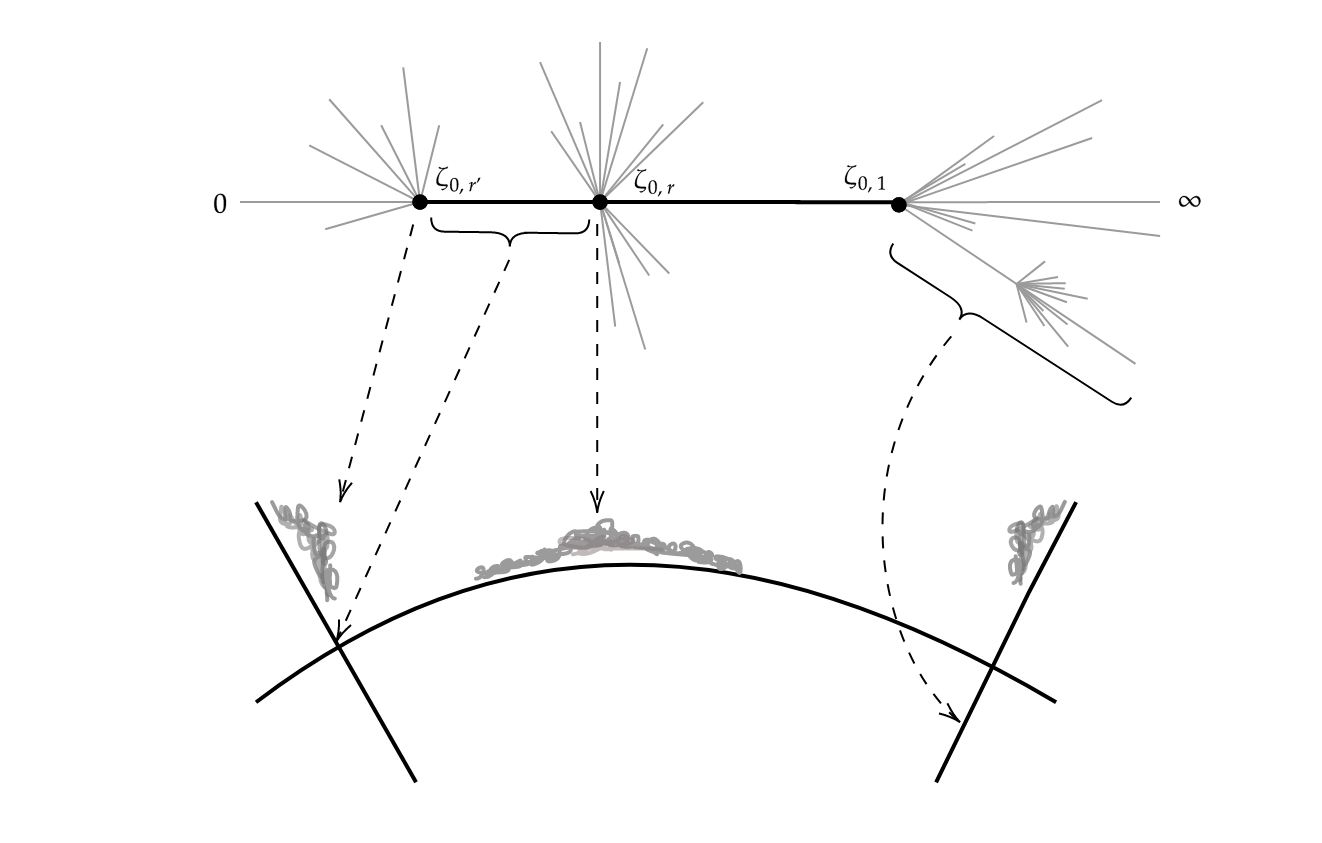
\includegraphics[width=0.8\textwidth]{Images/semistable.png}
    \caption{The relationship between a skeleton induced by a semistable vertex set and the corresponding formal model. The top image shows the analytic projective line with the skeleton in bold. Dashed arrows indicate the reduction map. 
    Clouds above each projective line in the semistable model shown at the bottom indicate the generic point of the component.}
    \label{fig:semistable}
\end{figure}

In the general case, we begin by fixing an edge $e$.
Suppose the open annuli in the semistable decomposition are $A_0, \dots, A_n$, and by permuting indices that $e$ contains $\rho(A_0)$.
There are two cases to consider. 

If $e$ has a vertex $x$ which is not contained in any other edge in $\Sigma$ \footnote{Note that this case is missing from the proof of  \parencite[Theorem 3.2.10]{bpr}.}, then we choose an open ball $B_x$ retracting to $x$.
It can be shown that $Y = \rho^{-1}(x)$ is an affinoid domain, by arguing that $\anl{X} \backslash (\bigcup_{i = 0}^{n} A_i)$ is an affinoid domain using \cref{complementaffinoid} and using the fact that $\rho^{-1}(x)$ is a connected component.
We let $\mathfrak{C}_x$ be the canonical model for $\rho^{-1}(x)$.
Similarly, we can show that $Y' = \rho^{-1}(e) \backslash B_x$ is an affinoid domain with canonical model $\mathfrak{Y}$, by arguing that it is a connected component of $\anl{X} \backslash (B_x \cup \bigcup_{i = 1}^{n} A_i)$.
The intersection $Y \cap Y'$ is then modelled by isomorphic open formal subschemes of $\mathfrak{C}_x$ and $\mathfrak{Y}$, giving the appropriate gluing data.

In the second case, both vertices of $e$ are contained in other edges of $\Sigma$.
We again argue that $\rho^{-1}(e)$ is an affinoid domain since it is a connected component of $\backslash (\bigcup_{i = 1}^{n} A_i)$.
Let $\mathfrak{D}$ be the canonical model; then the formal fibers above closed points are given by connected components of $\rho^{-1}(e) \backslash \{x, y \}$.
These connected components are the open balls which retract to either $x$ or $y$, or $A_0$, so it follows that $\mathfrak{D}$ consists of two irreducible components intersecting at an ordinary double point $\xi$.
If $\mathfrak{C}$ is the irreducible component whose generic fiber has formal fiber $\{x\}$, then the canonical model for $\rho^{-1}(x)$ is given by $\mathfrak{C} \backslash \{\xi\}$.
If $e'$ is another edge with vertex $x$, then $\rho^{-1}(e) \cap \rho^{-1}(e') = \rho^{-1}(x)$, so that by repeating this procedure for $e'$, we obtain the necessary gluing data for the respective canonical models.

A natural question to ask now is whether any $k$-analytic curve has a semistable decomposition, and hence, a skeleton. 
The following theorem answers this positively in the algebraically closed case.

\begin{theorem}[Semistable Reduction Theorem] \parencite[Theorem 7.1]{boschlutkebohmert}
    Let $X$ be a smooth, projective, geometrically connected curve over $k$, where $k$ is not necessarily algebraically closed.
    Then, there exists a finite extension $k \subset k'$ with valuation ring $R'$ such that $\anl{(X \times_{k} k')}$ admits a semistable formal $R'$-model.
\end{theorem}

Hence, when $k$ is algebraically closed, we deduce by our correspondence that a $k$-analytic curve $\anl{X}$ has a semistable vertex set.



\chapter{Skeleta in Higher Dimensions} \label{chapter4}

Throughout this section, let $k$ be the fraction field of a discrete valuation ring $R$ which has uniformizer $\pi$. 
We will denote by $X$ a smooth, proper, connected $k$-scheme.
Once again, we will use the notion of models to study $k$-analytic spaces, but it is more convenient here to use schemes as opposed to formal schemes.
The aim of this section is to generalise the notion of skeleta to higher dimensions.

\section{$R$-Models}

To begin, we define an \textit{$R$-model} for $X$ to be a flat, proper, $R$-scheme $\model$ equipped with an isomorphism $\model_k \cong X$, where $\model_k = \model \times_{R} k$ denotes the generic fiber.
The assumption that the model is proper may be weakened, but we include it here to simplify the presentation.
A morphism of $R$-models $h: \model' \to \model$ is a morphism of $R$-schemes which is compatible with the isomorphisms $\model'_k \cong X$ and $\model_k \cong X$ in the following sense.
By the universal property of the fiber product, $h$ induces a morphism $h_k: \model'_k \to \model_k$.
We then require that the following diagram commutes, where the diagonal maps are the isomorphisms specified by the model.
\[
\begin{tikzcd}
        \model_k' \arrow[dr, "\sim", sloped] \arrow[rr,"h_k"] && \model_k \arrow[dl, "\sim", sloped] \\
        & X 
\end{tikzcd}    
\]

For an $R$-model $\model$, we may consider the space $\hat{\model}_{\eta}$, which is isomorphic to $\anl{X}$ due to the properness assumption.
We find that $\hat{\model}_{s} \cong \model_s$, and so we obtain a map $\operatorname{red}_{\model} : \hat{\model}_{\eta} \to \model_s$.
Fixing a point $x \in \hat{\model}_{\eta}$ and choosing $U = \spec A \subset \model$ to be such that $x \in \hat{U}_{\eta}$, we find that $\red{\model}{x}$ corresponds to the prime ideal of $A$ given by $\{ a \in A \; \vert \; |a|_x < 1\}$.
We note that if $h: \model' \to \model$ is a morphism of $R$-models, then one sees that $h \circ \operatorname{red}_{\model'} = \operatorname{red}_{\model}$.

Furthermore, $x$ defines a multiplicative seminorm on $\sheaf_{\model, \red{\model}{x}}$.
Indeed, if $f \in \sheaf_{\model, \red{\model}{x}}$, then $f$ is regular on some neighbourhood $U = \spec A$, and we find that $x$ induces a seminorm on $A$.
To see that this is well-defined, let $x \in V \subset U$, with $U = \spec A$ and $V = \spec A'$.
The open immersion $V \to U$ induces an open immersion $\anl{V_k} \to \anl{U_k}$ by \parencite[Proposition 3.4.6]{berk1}, and a morphism $\hat{V}_{\eta} \to \hat{U}_{\eta}$.
By considering the following diagram and replicating the proof of \cref{lemma:affinecaseisaffinoid}, we see that that $\hat{V}_\eta \to \hat{U}_{\eta}$ is the embedding of an affinoid domain.
\[
\begin{tikzcd}
 & \hat{V}_{\eta} \arrow[r, overlay] \arrow[d, overlay] & \hat{U}_{\eta} \arrow[d, overlay] \\
 & \anl{V_k} \arrow[r, overlay] & \anl{U_k}
\end{tikzcd}
\]
It follows from this observation that the following diagram commutes, where the top map is the restriction map, showing that the seminorm is well-defined.
\[
\begin{tikzcd}
        A \arrow[dr, overlay] \arrow[rr,"\operatorname{res}", overlay] && A' \arrow[dl, overlay] \\
        & \resfield 
\end{tikzcd}    
\]

\section{The Skeleton of a Strict Normal Crossings Model}

\subsection{Strict Normal Crossings Divisors}

The notion of a strict normal crossings model can be seen as a generalisation of semistable formal models to the current setting.

\begin{defn}\parencite[Chapter 9, Definition 1.6]{liu}
    Let $D$ be an effective Cartier divisor on a locally Noetherian scheme $X$. Let $\{D_i\}_{i \in I}$ be the irreducible components of $D$ considered as reduced subschemes. Then, the following are equivalent.
    \begin{enumerate}
        \item For each $p \in D$, the ring $\sheaf_{X, p}$ is a regular ring with a regular system of parameters $z_1, \dots, z_n$ such that $D$ is locally given by the vanishing of the monomial $z_1^{N_1} \cdots z_r^{N_r}$ for some $r \leq d$ and positive integers $N_1, \dots, N_r$.
        \item Each $D_i$ is an effective Cartier divisor and the scheme theoretic intersection $\bigcap_{j \in J} D_j$ is a regular subscheme of codimension $|J|$ in $X$, where $J \subset I$ is finite.
    \end{enumerate}
    If $D$ satisfies the above, it is called a \textit{strict normal crossings divisor} on $X$. 
\end{defn}

The special fiber $\model_{s}$ of an $R$-model is a closed subscheme whose ideal sheaf is locally generated by the element $\pi$. 
A module over a discrete valuation ring is flat if and only if the uniformizer $\pi$ is not a zero divisor, hence $\model_{s}$ is an effective Cartier divisor on $\model$.

A regular $R$-model $\model$ where $\model_s$ is a strict normal crossings divisor is called an \textit{snc model}.
For brevity, an \textit{snc system of parameters} will refer to a regular system of parameters at a point $z \in \model_s$ such that $\model_s$ is locally given by the vanishing of the monomial $z_1^{N_1} \cdots z_r^{N_r}$ and $z_i = 0$ is a local equation for the irreducible component $D_i$.
Note that we allow each irreducible component, when considered as a prime divisor, to appear with multiplicity.

In general, it is not known whether snc models exist for a given scheme $X$.
Starting from a proper $R$-model, we may produce an snc model using \textit{resolution of singularities}; here, we state a stronger version which will be useful for some proofs in this chapter.

\begin{theorem}[Embedded Resolution of Singularities] \label{resofsing} \parencite{hironaka, hauserresolution, cossart1, cossart2}
Let $(W, Y)$ be a pair such that $Y$ is a divisor on an excellent, reduced scheme $W$.
Assume $W$ has characteristic zero, or that $W$ has dimension at most three and is separated.
Then, there exists a proper birational morphism $\Pi: W' \to W$ such that $W'$ is regular, the total transform of $Y$ is a strict normal crossings divisor in $W'$ and $\Pi$ is an isomorphism outside of $\operatorname{Sing}(Y) \cup \operatorname{Sing}(W)$, where $\operatorname{Sing}(\cdot)$ denotes the singular locus of a scheme.
\end{theorem}

For our purposes, the algebraic condition of excellence always holds since any complete local Noetherian ring is excellent, and a finitely generated algebra over an excellent ring is excellent.
Proper $R$-models exist due to Nagata's compactification theorem, and then \Cref{resofsing} may be used, assuming that $X$ satisfies the relevant conditions, to produce an snc model from a proper $R$-model $\model$, by applying the theorem to the pair $(\model, \model_s)$.
In general, we will assume the existence of an snc model for $X$.

To begin, we explore how blow-ups allow us to construct snc models from existing ones.
Throughout the chapter, we will freely use the following standard facts about blow-ups, references for which can be found in \parencite[Chapter 8]{liu}.

Firstly, if $X$ is a scheme and $\Pi: X' \to X$ is the blow-up along some center $Z$, then for any open $U \subset X$, $\Pi^{-1}(U)$ is isomorphic to the blow-up of $U$ along $U \cap Z$.
Hence, blow-ups can be computed locally and patched together.

Assume next that $U = \spec A$ is a Noetherian, integral affine scheme and the blow-up $U' \to U$ has center cut out by the ideal $I = (f_1, \dots, f_n)$, where $f_i \neq 0$.
Then, $U'$ is covered by affines of the form $\spec A_i$, where $A_i \subset \operatorname{Frac}(A)$ is the $A$ subalgebra of $\operatorname{Frac}(A)$ generated by $f_j/f_i$, for $j \neq i$.
It follows from these facts that if $X$ is additionally a flat $R$-scheme, then $X'$ is also a flat $R$-scheme.
If both $X$ and the center $Z$ are regular, then the blow-up of $X$ along $Z$ is also regular.

If $X$ is locally Noetherian, the blow-up along a closed subscheme cut out by a quasi-coherent ideal sheaf is a proper morphism, and $\Pi$ restricts to an isomorphism away from the center of the blow-up.
Furthermore, a composition of proper morphisms is proper, hence a sequence of blow-ups gives a a proper morphism.

\begin{prop}\label{lemma:blowupsnc}
    Let $\model$ be an snc model and $Z$ a closed subscheme such that one of the following holds:
    \begin{enumerate}
        \item $Z = \{z\}$ for a closed point $z$, such that $z \in \model_s$;
        \item $Z$ is a connected component of an intersection $\cap_{i = 1}^{r} D_i$ of irreducible components of $\model_s$.
    \end{enumerate}
    Let $\Pi: \model' \to \model$ be the blow-up with center $Z$. Then $\model'$ is an snc model.
\end{prop}
\begin{proof}
    Assume we are in the first case.
    There is an isomorphism of the generic fibers $\model'_k \cong \model_k$ since the blow-up has center contained in the special fiber.
    We see that $\model'$ is a regular $R$-model by standard results on blow-ups. 
    
    We now show that $\model'_s = \model^{*}_s + E$ is an snc divisor, where $\model^{*}_s$ denotes the strict transform of $\model_s$ and $E$ is the exceptional divisor. 
    It suffices to work in an affine neighbourhood $U = \spec A$ of $z$, in which case the blow-up $U' \to U$ with center $z$ may be computed as follows. 
    Let $z_1, \dots, z_n$ be an snc system of parameters at $z$, so that by shrinking $U$ as necessary, $z$ corresponds to a maximal ideal of $A$ generated by $(z_1, \dots, z_n)$ and $\model_s$ is given by the vanishing of the function $z_1^{N_1} \cdots z_r^{N_r}$ in $U$.
    The blow-up $U' \to U$ can be covered by charts $U_i = {\spec A_i}$ where 
    \[A_i := A[T_1, \dots, \hat{T_i}, \dots T_n]/(T_j z_i - z_j)_{j \neq i}.\] 
    We show that $\model'_{s} \cap U_i$ is a divisor with strict normal crossings in each $U_i$.
    
    Consider the case where $i = r$; the other cases are similar. 
    Then, if $\mathfrak{J}$ is the ideal of $A$ generated by $\pi$, we have
    \begin{align*}
        \mathfrak{J} \cdot A_i & = (z_1^{N_1} \cdots z_r^{N_r}) \cdot A_i
        = \left(\left(\frac{z_1}{z_r}\right)^{N_1} \cdots \left(\frac{z_{r-1}}{z_r}\right)^{N_{r - 1}} \cdot z_r^{N_1 + \dots + N_r} \right)
        = \left(T_1^{N_1} \cdots T_r^{N_r} \cdot z_r^{N_1 + \dots + N_r} \right).
    \end{align*}
    Since the exceptional divisor is given by the vanishing of $z_r$ in the chart $U_r$, it follows that the strict transform $\model^{*}_{s}$ is cut out by the monomial $T_1^{N_1} \cdots T_{r - 1}^{N_{r -1}}$ in $U_r$.
    A prime component is given by the vanishing of $T_j$, and hence is the strict transform of the prime component $D_j$ of $\model_s$ given by the vanishing of $z_j$.
    Since the strict transform of $D_j$ is isomorphic to the blow-up of $D_j$ with center $z$, we see that it is regular.
    To show regularity of the intersections, it suffices to consider the subscheme $\spec A_i/(T_{i_1}, \dots, T_{i_m}, z_r)$ for some set of indices $i_1, \dots, i_m$.
    We assume for ease of notation that the indices are $\{1, \dots, m\}$, for some $m < r$.
    We now find that:
    \begin{align*}
        & \spec A_i/(T_1, \dots, T_m, z_r) \\ 
        & \cong \spec A[T_1, \dots, \hat{T_r}, \dots, T_n]/(T_jz_r - z_j, T_1, \dots, T_m, z_r)_{j \neq r} \\
        & \cong \spec (A/(z_1, \dots, z_n))[T_{m + 1}, \dots, T_n] \\
        & \cong \spec K[T_{m + 1}, \dots, \hat{T_r}, \dots, T_n].
    \end{align*}
    where $K$ is a field.
    Hence, we see that the intersection is regular and of codimension $n - (n - m - 1) = m + 1$, as required.
    
    The proof of the second case is done via a similar computation.
\end{proof}

\subsection{Monomial and Divisorial Points}

Let $\model$ be an snc model for $X$.
Using the notation as above, if $\xi$ is a generic point of some connected component of an intersection $\cap_{i = 1}^{r} D_i$ of $\model_s$, then there exists an snc system of parameters $z_1, \dots, z_r$ and a unit $u$ in $\sheaf_{\model, \xi}$ such that $\pi = u z_1^{N_1} \cdots z_r^{N_r}$ for some positive integers $N_1, \dots, N_r$. 
The aim of this section is to see how the special fiber identifies a subset of points of $\hat{\model}_{\eta}$, known as \textit{monomial and divisorial} points.

To begin the construction of such points, we require the following lemma, which can be seen as a generalisation of the idea that for a local ring $A$ with a principal maximal ideal $\maxideal = (\pi)$, every element of the $\maxideal$-adic completion $\hat{A}$ can be written as a power series in $\pi$.

\begin{lemma}\parencite[Lemma 2.4.4]{MN}
    Let $z_1, \dots, z_n$ be a regular system of parameters for the maximal ideal of $\sheaf_{\model, \xi}$. 
    Let $\hat{\sheaf}_{\model, \xi}$ be the completion with respect to the maximal ideal. 
    Then, every element $f \in \hat{\sheaf}_{\model, \xi}$ can be written in the form
    \begin{equation}\label{eqn:admissibleexpansion}
        f = \sum_{\beta \in \mathbb{Z}^n_{\geq 0}} c_{\beta} z^{\beta}
    \end{equation}
    where each $c_{\beta}$ is zero or a unit in $\hat{\sheaf}_{\model, \xi}$.
    Such an expansion is called an \textit{admissible expansion} for $f$.
\end{lemma}
\begin{proof}
    The proof is reproduced from \textit{loc. cit.} here.
    Denote by $\maxideal_{\xi}$ the maximal ideal of $\hat{\sheaf}_{\model, \xi}$.
    Fix an element $f \in \hat{\sheaf}_{\model, \xi}$ and assume that $f$ lies in $\maxideal_{\xi}$ since otherwise we are done. 
    Now let $i \geq 1$ and assume that for all $j \leq i$, any $f' \in \hat{\sheaf}_{\model, \xi}$ has an expansion of the form:
    \[
        f' = f'_i + \left( \sum_{|\beta| = i} c_\beta z^{\beta} \right)
    \]
    where $f'_i$ is an element which has an admissible expansion and each $c_\beta$ is some element of $\hat{\sheaf}_{\model, \xi}$. 
    In particular, for $j = i$, $f$ has such an expansion:
    \[
        f = f_i + \left( \sum_{|\beta| = i} c_\beta z^{\beta} \right).
    \]
    For each coefficient $c_\beta$ in the expansion for $f$, we may apply the assumption with $j = 1$, so that we can write $f$ in the form:
    \begin{align*}
        f & = f_{i} + \sum_{|\beta| = i} (c_{\beta, i} + d_{1} z_1 + \dots + d_n z_n) z^{\beta} \\
        & = \left(f_i + \sum_{|\beta| = i} c_{\beta, i} z^{\beta}\right) + \left(\sum_{|\beta| = i} d_1 z_1 z^{\beta} + \dots + d_n z_n z^{\beta}\right) \\
        & = f_{i + 1} + g_{i + 1}
    \end{align*}
    where $c_{\beta, i}$ is an element admitting an expansion of the form \ref{eqn:admissibleexpansion}.
    We see that $f_{i + 1}$ is an element with an admissible expansion while $g_{i + 1}$ is a monominal in $z_1, \dots, z_n$ of degree $i + 1$.
    Furthermore, the coefficients of $f_{i + 1}$ and $f_{i}$ agree in degree $ < i$.
    Iterating this gives an admissible expansion for $f$.
\end{proof}

\begin{lemma}\label{lemma:zerouniqueexpansion} \parencite[Prop. 2.4.6]{MN}
    The element $0 \in \hat{\sheaf}_{\model, \xi}$ has a unique admissible expansion, where all coefficients are $0$.
\end{lemma}
\begin{proof}
    Let
    \[
        0 = \sum_{\beta \in \ZZ^{r}_{\geq 0}} d_{\beta} z^{\beta}
    \]
    be an admissible expansion for $0$.
    The claim is that for each $\beta$, $d_{\beta}$ lies in the maximal ideal $\maxideal$ of $\hat{\sheaf}_{\model, \xi}$, hence must be zero.
    We show this by inducting on $|\beta|$, and using the following result from commutative algebra.
    \begin{lemma}\parencite[Prop. 11.20]{AM}
        Let $z_1, \dots, z_r$ be a regular system of parameters for a local ring $A$ with maximal ideal $\maxideal$ and $f(t_1, \dots, t_r)$ a homogeneous polynomial of degree $s$ with coefficients in $A$. 
        Assume that $f(z_1, \dots, z_r) \in \maxideal^{s + 1}$. 
        Then all coefficients of $f$ lie in $\maxideal$.
    \end{lemma}
    In the base case, we have that $d_{0}$ must lie in the maximal ideal, since
    \[
        d_{0} = - \sum_{|\beta| > 1} d_{\beta} z^{\beta}.
    \]
    Assuming that $d_{\beta} = 0$ for all $\beta$ such that $|\beta| \leq s$ for some $s \geq 0$, we consider the homogeneous polynomial of degree $s + 1$ given by:
    \[
        f = \sum_{|\beta| = s + 1} d_{\beta} t^{\beta}.
    \]
    The parameters $z_1, \dots, z_r$ generate $\maxideal$ and we must have that $f(z_1, \dots, z_r)$ lies in $\maxideal^{s + 1}$ by the inductive hypothesis and rearranging the expansion.
    Hence, all coefficients lie in $\maxideal$ by the lemma.
\end{proof}

The utility of an admissible expansion is the following.
Firstly, note that for any $f \in \sheaf_{\model, \red{\model}{x}}$ for a point $x \in \hat{\model}_{\eta}$, $v_x(f) \geq 0$. 
From this we observe that if $f$ is a unit in $\sheaf_{\model, \red{\model}{x}}$, then $v_x(f) = -v_x(f^{-1})$, so $v_x(f) = 0$.
The same then holds true for $\hat{\sheaf}_{\model, \red{\model}{x}}$.
Hence, finding an admissible expansion for an element $f \in \sheaf_{\model, \red{\model}{x}}$ as in \cref{eqn:admissibleexpansion}, we see that 
\begin{equation}\label{equationforx}
    v_x(f) \geq \min \{ \alpha \cdot \beta \; \vert \; \beta \in \ZZ_{\geq 0}^{n}, c_{\beta} \neq 0 \}
\end{equation}
where $\alpha \cdot \beta$ denotes the dot product, and $\alpha = (v_x(z_1), \dots, v_x(z_n))$.
Due to the equation $\pi = u z_1^{N_1} \cdots z_r^{N_r}$, we must have that $v_x(z_1) N_1 + \cdots v_x(z_r) N_r = 1$.
These ideas lead to the construction of `monomial points', which are the points where \cref{equationforx} is an equality.

\begin{prop}\label{monomialpoint} \parencite[Prop. 2.4.6]{MN}
    Let $D_1, \dots, D_r$ be irreducible components of $\model_s$, and $\xi$ the generic point of a connected component of $\cap_{i = 1}^{r} D_i$.
    Let $N_i$ be the multiplicity of $D_i$ in $\model_s$ and let $\alpha = (\alpha_1, \dots, \alpha_r) \in \RR^{r}_{\geq 0}$ be such that $\alpha_1 N_1 + \dots + \alpha_r N_r = 1$.
    Then, there exists a point $x \in \hat{\model}_{\eta}$ inducing a valuation $v_{x}: K(X)^{\times} \to \RR$ such that for each $f \in \sheaf_{\model, \xi}$ and any admissible expansion of $f$ as in \cref{eqn:admissibleexpansion}, we have:
    \[
        v_{x}(f) = \min \{ \alpha \cdot \beta \; \vert \; \beta \in \mathbb{Z}_{\geq 0}^m, c_{\beta} \neq 0\}.
    \]
     The point $x$ is then called a \textit{monomial point} with presentation $(\model, (D_1, \dots, D_r), \xi, \alpha)$.
\end{prop}
\begin{proof}
    We give an alternative proof from the one presented in \textit{loc. cit.}.

Firstly, assume by permuting indices that $\alpha = (\alpha_1, \dots, \alpha_{r'}, 0, \dots, 0)$, where $\alpha_1, \dots, \alpha_{r'}$ are non-zero, for some $r' \leq r$.

Define for each $\alpha \in \mathbb{R}^r_{\geq 0}$ and $w \in \RR$ the ideal $I_{\geq w}$ of $\hat{\sheaf}_{\model, \xi}$ generated by the monomials $z^{\beta}$ such that $\alpha \cdot \beta \geq w$, and the ideal $I_{> w}$ generated by the monomials $z^{\beta}$ such that $\alpha \cdot \beta > w$.
Denoting by $\kappa$ the residue field of $\hat{\sheaf}_{\model, \xi}$, the claim is that $I_{\geq w} / I_{> w}$ is a $\kappa$ vector space with a basis given by $z^{\beta}$ where $\alpha \cdot \beta = w$.
To see this, first note that if $\alpha \cdot \beta = w$ for some $\beta$ and $w$, then $z^{\beta} \in I_{\geq w} \backslash I_{> w}$.
Indeed, suppose that $z^{\beta} \in I_{> w}$; then, we may write $z^{\beta} = c_1 z^{\beta_1} + \cdots + c_n z^{\beta_n}$, and, choosing admissible expansions for each $c_i$, we may find an admissible expansion
\[
    z^{\beta} + \sum_{\alpha \cdot \gamma > w} c_{\gamma} z^{\gamma} = 0.
\]
By, \cref{lemma:zerouniqueexpansion}, each coefficient in the admissible expansion must be zero, giving a contradiction.
Hence, the classes of the elements $z^{\beta}$ give a generating set for $I_{\geq w} / I_{> w}$.
A similar argument shows that any finite sum \[ c_1 z^{\beta_1} + \dots + c_m z^{\beta_m} \] where each $c_i$ is a unit, is not contained in $I_{> w}$, so that the classes of the elements $z^{\beta}$ with $\alpha \cdot \beta = w$ form a basis for $I_{\geq w}/I_{> w}$.

For each element $f$ of $\hat{\sheaf}_{\model, \xi}$, there exists some $w$ such that $f \in I_{\geq w} \backslash I_{> w}$, which must be unique since $\RR$ is totally ordered.
To see this, fix an admissible expansion for $f$ with coefficients $c_{\beta}$ and let $v = \min \{ \alpha \cdot \beta \; | \; c_{\beta} \neq 0 \}$. 
We can then write
\begin{align*}
    f & = \sum_{\alpha \cdot \beta = v} c_{\beta} z^{\beta} + \sum_{\alpha \cdot \beta > v} c_{\beta} z^{\beta} \\
    & = f' + f''.
\end{align*}
The ideal $I_{> v}$ is closed in the $\maxideal_{\xi}$-adic topology; for this it suffices to show that
\[
    \bigcap_{i > 0} (I_{> v} + \maxideal_{\xi}^{i}) \subset I_{> v}.
\]
This follows from the fact that $\maxideal^{i}_{\xi}$ is generated by monomials of degree $i$ in the $z_1, \dots, z_n$, so  for $i$ large enough, $\maxideal^{i}_{\xi} \subset I_{> w}$.
A similar argument shows that $I_{\geq v}$ is closed.
It follows from this that $f'' \in I_{> v}$ and $f' \in I_{\geq v}$, and by considering reductions modulo $I_{> v}$ we see that $f \not\in I_{> v}$.
Hence $v$ is the unique real number such that $f \in I_{\geq v} \backslash I_{> v}$, and in particular $v_x$ is independent of the choice of admissible expansion.

Since ideals are closed under addition, we find that $v_x(f + g) \geq \min \{ v_x(f), v_x(g) \}$.
Next, let $\overline{f}$ be the reduction of $f$ modulo $I_{> v}$, and write
\[
    \overline{f} = \sum_{\alpha \cdot \beta = w} d_{\beta} z^{\beta}
\]
where $d_{\beta} \in \kappa$.
We define $\Gamma_f$ as follows: for each choice of $\beta_1, \cdots, \beta_r$ such that $\alpha_1 \beta_1 + \dots + \alpha_{r'} \beta_{r'} = v$, $\beta = (\beta_1, \cdots, \beta_r)$ is in $\Gamma_f$ if $\beta_{r' + 1} + \dots + \beta_{r}$ is minimal amongst all possible choices of $\beta_{r' +1}, \dots, \beta_{r}$ such that $d_{\beta} \neq 0$.
We then define the polynomial
\[
    f_{\alpha} = \sum_{\beta \in \Gamma_f} d_{\beta} z^{\beta}.
\]
Then, we can view $f_{\alpha}$ as an element of $\kappa[z_1, \dots, z_n]$.
To show $v_x(f \cdot g) = v_x(f) + v_x(g)$, we now fix admissible expansions for $f$ and $g$, and a computation shows that $(f \cdot g)_{\alpha} = f_{\alpha} \cdot g_{\alpha}$, where the latter product is taken in the ring $\kappa[z_1, \dots, z_n]$.

Since $\pi = u \cdot z_1^{N_1} \cdots z_r^{N_r}$ is an admissible expansion, $v_x(\pi) = \alpha_1 N_1 + \cdots + \alpha_r N_r = 1$. 
Hence, $v_x$ extends the valuation on $k$. 
We conclude by noting that although $v_x$ is currently only defined on the local ring $\sheaf_{\model, \xi}$, it extends to a valuation on $K(\model) \cong K(X)$ by setting $v_x(f/g) = v_x(f) - v_x(g)$.
\end{proof}

Let $\xi$ be the generic point of a connected component of $\cap_{i = 1}^{r} D_r$, and suppose $\alpha$ has zero entries.
Then we may, after permuting indicies, assume that $\alpha = (\alpha_1, \dots, \alpha_{r'}, 0, \dots, 0)$ with $\alpha_1, \dots, \alpha_{r'}$ non-zero.
Then, the formula for $v_x$ shows that it is also the monomial point with presentation \[(\model, (D_1, \dots, D_{r'}), \xi', \alpha')\] where $\alpha' = (\alpha_1, \dots, \alpha_{r'})$ and $\xi'$ is the generic point of the connected component of $\cap_{i = 1}^{r'} D_i$ which contains $\xi$.

When $\xi$ is the generic point of an irreducible component $D$, then $\sheaf_{\model, \xi}$ is a discrete valuation ring with fraction field equal to $K(X)$. 
In this case, the valuation on $K(X)$ such that the valuation ring is $\sheaf_{\model, \xi}$ coincides with the valuation given by the monomial point corresponding to the data $(\model, D, \xi, \alpha = 1)$.
The point is then called a \textit{divisorial point} associated to the data $(\model, D)$.

Note that a point which is monomial with respect to a given model may in fact be divisorial with respect to another snc model. 
The following lemma and proposition form the contents of the proof of \parencite[Prop. 2.4.11]{MN}, and characterize when such a case occurs.

\begin{lemma} \label{blowupintersection}
    Let $D_1, \dots, D_r$ be prime components of $\model_s$ for some snc model $\model$ and $\xi$ the generic point of a connected component of $D_1 \cap \dots \cap D_r$. 
    Let $\model' \to \model$ be the blow-up at the closure of $\xi$.
    If $x \in \hat{\model}_{\eta}$ is a point with monomial presentation $(\model, (D_1, \dots, D_r), \xi, \alpha)$, then $x$ is also monomial with respect to $\model'$.
    If $\alpha = (\alpha_1, \dots, \alpha_r)$ is such that $\alpha_1$ is the minimal coordinate, $D'_2, \dots, D'_r$ are the strict transforms of $D_2, \dots, D_r$ and $E$ is the exceptional divisor, then $x$ has monomial presentation $(\model', (E, D'_2, \dots, D'_r), \xi', \alpha')$ where $\xi'$ is the generic point of $E \cap D'_2 \cap \dots \cap D'_r$  and $\alpha'$ is the tuple
    \[
        \alpha' = (\alpha_1, \alpha_2 - \alpha_1, \dots, \alpha_r - \alpha_1).
    \]
\end{lemma}
\begin{proof}
    By \cref{lemma:blowupsnc}, $\model'$ is an snc model.
    Let $U = \spec A$ be an affine neighbourhood of $\xi$ such that if $z_1, \dots, z_r$ is an snc system of parameters, then $\xi$ corresponds to the prime ideal $(z_1, \dots, z_r)$ of $A$.
    We have that $\red{\model'}{x}$ is the point of $\spec A[T_2, \dots, T_r]/(T_jz_1 - z_j) \subset \model'$ corresponding to the prime ideal $(z_1, T_2, \dots, T_r)$.
    The vanishing of the elements $T_j$ define the strict transforms $D'_j$ of $D_j$ for each $2 \leq j \leq r$, and the vanishing of $z_1$ defines the exceptional divisor.
    In particular, we can take $z_1, T_2, \dots, T_r$ to be an snc system of parameters.
    
    Now, let $x'$ be the monomial point corresponding to the data $(\model', (E, D'_2, \dots, D'_r), \xi', \alpha')$ as in the statement of the lemma.
    Since $\red{\model}{x'} = \red{\model}{x}$, to show that $x' = x$, it suffices to show that for all $f \in \sheaf_{\model, \red{\model}{x}}$, $v_x(f) = v_{x'}(f)$.
    
    Fix $f \in \sheaf_{\model, \red{\model}{x}}$.
    Let
    \[
        f = \sum c_{\beta} z_1^{\beta_1} \cdots z_r^{\beta_r}
    \]
    be an admissible expansion for $f$ in $\hat{\sheaf}_{\model, \red{\model}{x}}$.
    We note that 
    \[
        f = \sum c_{\beta} z_1^{\beta_1 + \dots + \beta_r} T_2^{\beta_2} \cdots T_r^{\beta_r}
    \]
    gives an admissible expansion for $f$ in $\hat{\sheaf}_{\model, \red{\model'}{x'}}$.
    It follows immediately from the formulae for $v_x$ and $v_{x'}$ that $v_x(f) = v_{x'}(f)$.
 \end{proof}

\begin{prop} \label{monomialisdivisorial} \parencite[Proposition 2.4.11]{MN}
    A monomial point $x$ of $\hat{\model}_{\eta}$ with a monomial presentation \[(\model, (D_1, \dots, D_r), \xi, \alpha)\] is divisorial if the entries of $\alpha$ are rational.
\end{prop}
\begin{proof}
    Let $\model' \to \model$ be the blow-up at the closure of $\xi$.
    We may assume by permuting indices that $\alpha_1$ is the minimial coordinate. Then, by \cref{blowupintersection}, $\model'$ is an snc model where the monomial presentation of $x$ with respect to $\model'$ is such that $\alpha' = (\alpha_1, \alpha_2 - \alpha_1, \dots, \alpha_r - \alpha_1)$.
    Since each coordinate is rational, we can assume $\alpha$ is of the form $\left(\frac{a_1}{b}, \dots, \frac{a_r}{b} \right)$ for positive integers $a_1, \dots, a_r$ and some integer $b$.
    Hence, repeating this process and removing any zero entries, we reduce to the case where $r = 1$.
    This gives a divisorial presentation.
\end{proof}

\subsection{The Retraction to the Skeleton}

The skeleton $\sk{\model}$ of $\anl X$ induced by an snc model $\model$ is defined as the set of points of $\anl X$ which are monomial with respect to $\model$.
The space $\sk{\model}$ has a particularly elegant topological description as the \textit{dual complex} $\Delta(\model_s)$ of $\model_s$ \parencite[\S 2.4.2]{birgeom}.

Let $\{D_i\}_{i \in I}$ be the irreducible components of $\model_s$, and $J \subset I$ a non-empty finite subset.
Then, the dual graph $\Delta(\model_s)$ contains an $r$-simplex for each connected component of $\cap_{j \in J} D_j$, where $r = |J| - 1$.
We make the following identifications. 
Let $C \subset \cap_{j \in J} D_j$ and $C' \subset \cap_{k \in J'} D_k$ be two connected components corresponding to simplicies $E$ and $E'$. 
Then $E$ is a face of $E'$ if and only if we have $C' \subset C$.
There is a homeomorphism $\Phi: \Delta(\model_s) \to \sk{\model}$.
We describe the construction of the map and omit the proof that it gives a homeomorphism which may be found in \parencite[\S 2.4.4]{birgeom}.
Let $x \in \Delta(\model_s)$ be a point; if it is a vertex, then it corresponds to an irreducible component $D \subset \model_s$ and we map it to the divisorial point with presentation $(\model, D)$.
Otherwise, $y$ lies on the interior of a simplex corresponding to some connected component of an intersection $\cap _{j \in J} D_j$.
Let $r = |J|$, $\xi$ be the generic point of the component and let $(w_1, \dots, w_{|J|})$ be the coordinates of $y$ considered as a point on the simplex.
Then $w_1 + \dots + w_{r} = 1$, so $\alpha = \left({w_1}/{N_1}, \dots, {w_r}/{N_r} \right)$ is such that $\alpha_1 N_1 + \dots + \alpha_r N_r = 1$.
We then map $y$ to the monomial point with presentation $(\model, (D_1, \dots, D_r), \xi, \alpha)$.

The inclusion $\sk{\model} \subset \hat{\model}_{\eta}$ admits a continuous retraction $\rho_{\model} : \hat{\model}_{\eta} \to \sk{\model}$ \parencite[\S 3.1.5]{MN}. 
For any $x$, let $D_1, \dots, D_r$ be the irreducible components of $\model_s$ passing through $\red{\model}{x}$. 
Fix $1 \leq i \leq r$.
Letting $z_1, \dots, z_n$ be an snc system of parameters at $\red{\model}{x}$ such that $D_i$ is locally given by the vanishing of $z_i$, set $v_x(D_i) := v_x(z_i)$.
Note that $N_1v_x(z_1) + \cdots + N_r v_x(z_r) = v_x(\pi) = 1$, so that setting $\alpha = (v_x(z_1), \dots, v_x(z_r))$ and letting $\xi$ be the generic point of the connected component of $\cap_{i = 1}^r D_i$ which contains $\red{\model}{x}$, we set $\rho_{\model}(x)$ to be the point with monomial presentation $(\xi, \alpha)$ with respect to the model $\model$.
This is well-defined: the parameters $z_1, \dots, z_r$ are determined up to multiplication by a unit in $\sheaf_{\model, \red{\model}{\xi}}$, so if $z'_i$ is another function defining $D_i$ locally, then $z_i = u \cdot z'_i$ for some unit $u \in \sheaf_{\model, \red{\model}{\xi}}$.
Since $v_x(u) = 0$ it follows that $v_x(z_i) = v_x(z'_i)$.
We also see that $v_x(D) = v_{\rho_{\model}(x)}(D)$ for every prime component $D$ of $\model_s$ passing through $\red{\model}{x}$.
We remark for later use that the construction $v_x(D)$ extends to any divisor $D$ which is not supported on $\iota(x)$, by similarly choosing a local equation for $D$ at $\red{\model}{x}$.

The retraction map has the following properties, which we state without proof. 
Denote $y = \rho_{\model}(x)$, for any $f \in \sheaf_{\model, \red{\model}{x}}$. 
If $f \in \sheaf_{\model, \red{\model}{x}}$ is a function regular on some neighbourhood $U$ of $\red{\model}{x}$, then note that $U$ contains $\red{\model}{y}$ so that we may consider $|f|_y$. 
Then, $|f|_x \leq |f|_y$ for every $f \in \sheaf_{\model, \red{\model}{x}}$ \parencite[Prop. 3.1.6]{MN}. 
The following proposition shows that the retraction map is well-behaved with respect to blow-ups.

\begin{prop} \label{retractionsinversesystem} \parencite[Prop. 3.1.7]{MN}
    If $\model' \to \model$ is a proper morphism of snc models of $X$, i.e. a proper morphism of $R$-models where both $\model, \model'$ are snc, then $\rho_{\model} \circ \rho_{\model'} = \rho_{\model}$ and $\sk{\model} \subset \sk{\model'}$.
\end{prop}

In the case of curves, we have the following characterisation of the retraction points.

\begin{prop}\label{lemma:retractiondivisorial}
    Let $X$ be a curve and $x, y \in \hat{\model}_{\eta}$ be distinct points such that $\rho_{\model}(x) = \rho_{\model}(y)$. 
    Then, $\rho_{\model}(x)$ is a divisorial point.
\end{prop}
\begin{proof}
    Without loss of generality, we may assume that $y = \rho_{\model}(x)$ is a monomial point which is not divisorial with respect to $\model$.
    Let $(\xi, (\alpha_1, \alpha_2))$ be a monomial presentation for $y$ with respect to the model $\model$ and let $z_1, z_2$ be a regular system of parameters at $\red{\model}{x} = \red{\model}{y} =: \xi$, such that $\xi$ is the generic point of the intersection of the vanishing loci of $z_1$ and $z_2$. 
    It suffices to show that $|z_1^a|_y = |\pi^b|$ for some $a, b$, since then $\alpha_1$ and $\alpha_2$ must be rational and we can conclude using \cref{monomialisdivisorial}.
    
    Assume $x$ is not a type III point; then we are done, since $|\resfield^{\times}|/|k^{\times}|$ is a rank $0$ abelian group and hence for every element $r \in |\resfield^{\times}|$, we have $r^a \in |k^{\times}|$. for some $a \in \ZZ_{\geq 0}$
    
    Now, we assume that both $x$ and $y$ are type III points and proceed to assume that $\alpha_1$ and $\alpha_2$ are irrational.
    Since $x$ and $y$ are distinct, we can assume that there exists some $f \in \sheaf_{\model, \red{\model}{x}}$ such that $v_x(f) \neq v_y(f)$. 
    Choosing an admissible expansion for $f$:
    \[
        f = \sum c_{ab} z_1^{a} z_2^{b}
    \]
    we see that
    \begin{align*}
        v_x(f) &= v_x \left(\sum c_{ab} z_1^{a} z_2^{b} \right) \\
              &= \min \{ v_x(c_{ab}) + aN_1 \alpha_1 + bN_2 \alpha_2 \} \\
              &= \min \{ v_y(c_{ab}) + aN_1 \alpha_1 + bN_2 \alpha_2 \} \\
              &= v_x \left(\sum c_{ab} z_1^{a} z_2^{b} \right) \\
              & = v_y(f)
    \end{align*}
    where we have used the irrationality of $\alpha_1$ and $\alpha_2$ to sharpen the triangle inequality into an equality, and the fact that $v_x(c) = v_y(c) = 0$ for any unit $c \in \hat{\sheaf}_{\model, \red{\model}{x}}$.
    Hence, we arrive at a contradiction, so it follows that $\alpha_1$ and $\alpha_2$ are rational. 
\end{proof}

A corollary of the proof of \cref{lemma:retractiondivisorial} is that for any type III point $x$ monomial with respect to an snc model $\model$, we have that $\rho_{\model}^{-1}(x) = \{x\}$. 

We now consider how blow-ups of snc models affect the skeleton of a curve.
Let $\model$ be an snc model for a curve $X$, $D_1, D_2$ irreducible components of $\model_s$ and $z$ the closed point contained in a connected component of the intersection $D_1 \cap D_2$.
Let $\model' \to \model$ be the blow-up at $z$ and $\sigma$ the interval of $\sk{\model}$ corresponding to $z$.
Then, the simplicial structure of $\sk{\model'}$ is given by barycentrically subdividing $\sigma$ in $\sk{\model'}$.

To see this, let $E$ be the exceptional divisor and $D'_1$, $D'_2$ the strict transforms of $D_1$ and $D_2$ respectively. 
Firstly, if $\red{\model}{x}$ is the generic point of $E$, then it follows from \cref{blowupintersection} that 
    \[(\model, (D_1, D_2), z, (1/(N_1 + N_2), 1/(N_1 + N_2))\] 
is a monomial presentation for $x$. 
If $\red{\model}{x}$ is, without loss of generality, the generic point of $D'_1$, then $(\model, D_1)$ is a divisorial presentation for $x$.

Next, we consider a point $x$ such that $\red{\model'}{x} =: \xi$ is the generic point of an intersection $E \cap D'_2$, after possibly permuting the induces.
Hence, let $(\model', (E, D_2), \xi, \alpha)$ be a monomial presentation for $x$.
In this case, it follows from \cref{blowupintersection} that 
\[(\model, (D_1, D_2), z, (\alpha_1, \alpha_2 + \alpha_1))\] is a monomial presentation for $x$.
    
Hence, we have shown that $\sk{\model'} \subset \sk{\model}$, from which it follows that $\sk{\model'} = \sk{\model}$. 
Considering the simplicial structure, there is an extra vertex corresponding to the exceptional divisor, which is located in the barycenter of the $1$-simplex corresponding to the point $z$.

This is in fact a special case of the following more general theorem, which we present without proof. 

\begin{prop}\label{blowupintersectionskeleton}\parencite[Prop. 3.1.9]{MN}
    Let $D_1, \dots, D_r$ be irreducible components of $\model_s$, $\xi$ the generic point of a connected component of the intersection $D_1 \cap \dots \cap D_r$ and $\sigma$ the face of $\sk{\model}$ corresponding to $\xi$. If $\model' \to \model$ is the blow-up with center given by the closure of $\xi$, then $\sk{\model'} = \sk{\model}$, and the simplicial structure of $\sk{\model'}$ is obtained by adding a vertex to the barycenter of $\sigma$ and joining it to the faces of $\sigma$.
\end{prop}

Now let $\model$ be an snc model for a curve $X$, $D$ an irreducible component of $\model_s$ and $z$ a closed point on $D$ such that no other irreducible components pass through $z$.
Let $\model' \to \model$ be the blow-up centered at $z$.
In this case, $\sk{\model}$ is a strict subset of $\sk{\model'}$.
Consider a point $x \in \sk{\model'}$ such that the closure of $\red{\model'}{x}$ is contained in the exceptional divisor $E$. 
We have that $\red{\model}{x} = z$, hence $x$ is not monomial with respect to $\model$.
We can see that the simplicial structure of $\sk{\model'}$ is obtained by adjoining a line segment to a vertex of $\sk{\model}$: more precisely, the vertices of the line segment correspond to the divisorial points associated with $E$ and $D$, while the interior corresponds to the monomial points with presentation $(\model', (E, D), \xi, \alpha)$, for some $\alpha$.

Finally, we note the following proposition due to Berkovich and Thuillier shows that for an snc model $\model$, $\sk{\model}$ is a strong deformation retract of $\anl X$.

\begin{prop} \parencite[Theorem 3.26]{thuillier}
    There exists a continuous map 
    \[
        H: \hat{\model}_\eta \times [0, 1] \to \hat{\model}_\eta
    \]
    such that $H_0(x) = H(x, 0)$ is the identity map, $H_1(x) = H(x, 1)$ is the retraction map $\rho_{\model}$ and for all $t \in [0, 1]$, $H(x, t) = x$ for $x \in \sk{\model}$.
\end{prop}

Hence, for an snc model $\model$, the homotopy type of $\anl{X}$ is the same as that of the dual complex of $\model_s$, which admits a simplicial structure and is hence easier to analyse.
The proof of the prior theorem requires machinery which is outside of the scope of this report; a construction of the deformation retraction in a concrete example may be found in \parencite[\S 2.5]{birgeom}.

\section{The Structure of $k$-Analytic Spaces}

The primary goal of this section will be to prove \cref{thm:homeomorphism}, which essentially states that an analytic space $\anl X$ can be recovered by taking an inverse limit of skeleta.
In order for this result to hold, we assume that $X$ satisfies the conditions of the ambient scheme $W$ in our statement of resolution of singularities (\cref{resofsing}).

A key result in proving this is the fact that for any two distinct points $x$ and $y$ in $\anl X$, there exists an snc model $\model$ such that $\rho_{\model}(x) \neq \rho_{\model}(y)$. 
Before giving a proof of this theorem, we illustrate the strategy using the example of the analytic projective line.
To begin, $\model = \mathbb{P}^{1}_{R}$ is an snc model for $\projlinean$. 
The special fiber is simply the projective line over $\tilde{k}$ and the corresponding skeleta consists of a single type II point, corresponding to the norm on $k\{T\}$.
Consequently, we see that every point retracts to the same point. 

We split our analysis into two cases, depending on whether $\red{\model}{x}$ and $\red{\model}{y}$ are equal. 
In the first case, let $x$ be the point given by the seminorm $|f(T)|_x = |f(0)|$ for all $f \in k[T]$, and $y$ the point given by the seminorm $|f(T)|_x = |f(1)|$.
Both of these points lie in the closed disk $E(0, 1) = \berkspec{k\{T\}} \subset \projlinean$, so that the affine chart $\spec R[T] \subset \model$ contains $\red{\model}{x}$ and $\red{\model}{y}$.
Then, observe that $\resfield^{\circ\circ} \cap R[T]$ is the ideal $(\pi, T)$: if $f(T) = \pi \cdot g(T) + T \cdot h(T)$, then we may assume that $g(T) = c$ is a constant and compute:
\[
|f(T)|_x \leq \max\{ |\pi \cdot c|_x, |T \cdot h(T)|_x \} < 1.
\]
Conversely, if $f(T) = a_0 + \dots + a_n T^n$ is such that $|f(T)|_x < 1$, then: $|f(T)|_x = |a_0 + \dots + a_n T^n|_x = |a_0| < 1$, hence it follows that $a_0 \in (\pi)$ and hence $f(T) \in (\pi, T)$. 
Therefore, $\red{\model}{x}$ is the point of $\spec R[T]$ corresponding to the maximal ideal $(\pi, T)$.
A similar argument shows that $\red{\model}{y}$ is the point corresponding to the maximal ideal $(\pi, T - 1)$, and hence we are in the case $\red{\model}{x} \neq \red{\model}{y}$. 
It follows from \cref{lemma:blowupsnc} that performing a blow-up of $\model$ at either of the reduction points will give rise to an snc model $\model^{\prime}$; the claim is that $\rho_{\model^\prime}(x) \neq \rho_{\model^{\prime}}(y)$.

Choosing the point given by $(\pi, T)$ as the center of the blow-up, we find that the resulting scheme 
\[\model^\prime = \proj R[T][A, B]/(\pi B - T A)\] 
admits a covering by affine charts $U_{B} = \spec R[T, a]/(\pi - T a)$ and $U_{A} = \spec R[T, b]/(\pi b - T) \cong \spec R[b]$.
These affine charts are glued along the isomorphism \[\spec R[T, a, a^{-1}]/(\pi - T a) \cong \spec R[T, b, b^{-1}]/(\pi b - T)\] induced by the ring homomorphism sending $a \mapsto b^{-1}$.
Consequently, the special fiber is now given by the charts $\tilde{U}_{B} = \spec \tilde{k}[T, a]/(T a)$ and $\tilde{U}_{A} = \spec \tilde{k}[T, b]/(t) \cong \spec \tilde{k}[b]$ with the corresponding gluing. 
Geometrically, the blow-up has the effect of attaching a projective line to the origin of the affine line over $\tilde{k}$.
In particular, $\red{\model^{\prime}}{x}$ is now the point at infinity of the projective line in the special fiber.
Since the sets of irreducible components of the special fiber passing through $\red{\model'}{x}$ and $\red{\model'}{y}$ are disjoint, it follows that the points $\rho_{\model^\prime}(x)$ and $\rho_{\model^\prime}(y)$ are distinct.

We digress momentarily to analyse the generic fiber of $\model^\prime$.
The space $\hat{\model^{\prime}}_{\eta}$ is now formed by gluing $\berkspec{k\{T, a\}/(\pi - a T)}$ and $\berkspec{k\{T, b\}/(\pi b - t}$ along $\berkspec{k\{\pi^{-1} T, \pi T^{-1}\}}$.
Observe that the former affinoid space is an annulus with inner radius $\pi$ and outer radius $1$, while the latter is isomorphic to the closed disk $\berkspec{k\{b\}}$, which embeds into $\berkspec{k\{T\}}$ using the map $b \mapsto \pi^{-1} T$. Hence, it is identified with the closed disk of radius $\pi$, and the space $\hat{\model}^{\prime}_{\eta}$ is isomorphic to the closed unit disk $\berkspec{k\{T\}}$.

Now we consider a case where the specializations $\red{\model}{x}$ and $\red{\model}{y}$ are equal. 
For this, let $x$ be as before, and let $y$ be the point given by the norm on $k\{r^{-1} T\}$, where $r < 1$.
The earlier argument which showed that $\red{\model}{x}$ is the point of $\spec R[T]$ given by the ideal $(\pi, T)$ generalises to show that $\red{\model}{y}$ is also the point $(\pi, T)$.
Intuitively, we can think of this as a consequence of the fact that both $x$ and $y$ lie in the open disk $D(0, 1)$.

The goal now is to find a suitable center for a blow-up such that the reductions of the two points are distinct, hence reducing to the previous case.

Note that the regular function $f(T) = T + \pi^2$ is such that $|f|_x = |\pi^{2}| \neq |\pi| = |f|_y$.
Consider the subscheme $Z$ of $\model$ defined by the ideal $(\pi, T + \pi^2) = (\pi, T)$.
Blowing-up gives the same scheme computed above, but we note that both reduction points now lie in the chart $U_A$.
In particular, the points define multiplicative seminorms on the ring $R[T, b]/(\pi b - T)$, and $f/\pi = b + \pi$ is a regular function on the chart $U_A$.
We find that $|f/\pi|_x = |b + \pi|_x = |\pi|$, while $|b + \pi|_y = 1$, so it follows that the reduction points are now distinct.

To generalise these arguments, we must consider which aspects of the example above resulted in simplification which may in general be unreasonable to expect.

In the first case of our analysis, when the analytic space is not a curve, it may not be the case that one of the reduction points is closed.
In this case, we may try to take the closure of one of the reduction points as a center for the blow-up, but this center may contain singularities, so that the blow-up may not even be regular.
Consequently, to produce the desired snc model, we may invoke resolution of singularities.
If $\Pi: \model' \to \model$ is as in the statement of the theorem, then $\Pi^{-1}(\model_s) \cong \model'_s$.

In the second case, we wish to more generally find a function $f$ such that $|f|_x \neq |f|_y$ and either $|f|_x$ or $|f|_y$ is equal to $|\pi^{k}|$ for some $k$, so that we can then take the blow-up with center defined by the ideal $(\pi^{k}, f)$ in some neighbourhood of the reduction point.
Once again, the closure of the subscheme defined by this ideal may not be regular, leading us to further invoke resolution of singularities.

Equipped with these ideas, we formulate the following series of lemmas.


\begin{lemma}\label{rednotequal}
    Let $\model$ be an snc model and $x, y \in \hat{\model}_{\eta}$ distinct points such that $\rho_{\model}(x) = \rho_{\model}(y)$ but $\red{\model}{x} \neq \red{\model}{y}$.
    Then there exists a snc model $\model' \to \model$ such that $\rho_{\model'}(x) \neq \rho_{\model'}(y)$
\end{lemma}
\begin{proof}
    We may assume firstly that $\red{\model}{x} \not\in \overline{\{\red{\model}{y}\}}$. 
    Indeed, if we have both $\red{\model}{x} \in \overline{\{\red{\model}{y}\}}$ and $\red{\model}{y} \in \overline{\{\red{\model}{x}\}}$, then it follows that $\overline{\{\red{\model}{x}\}} = \overline{\{\red{\model}{y}\}} =: Z$.
    Hence, $\red{\model}{x} = \red{\model}{y}$ is the generic point of the irreducible closed subset $Z$, which is a contradiction.
    
    Now denoting $Z := \overline{\{\red{\model}{y}\}}$, we consider the blow-up $\model'' \to \model$ with center $Z$.
    In general, the subscheme $Z$ is not regular and hence $\model''$ is not guaranteed to be an snc model.
    We now perform a resolution of singularities of the pair $(\model'', \model_s'')$, resulting in a regular scheme $\model' \to \model''$.
    Since a blow-up is an isomorphism outside of its center, any singular points are contained within $\model_s''$.
    In particular, performing resolution of singularities induces an isomorphism of generic fibers $\anl{(\model_s')} \cong \anl{(\model_s'')}$.
    Furthermore, the special fiber of $\model'$ is given by the total transform of the special fiber of $\model''$.
    Hence, we see that $\model'$ is an snc model.
    
    Let $\Pi: \model' \to \model'' \to \model$ be the composition.
    We observe that $\red{\model'}{y}$ lies in $\Pi^{-1}(Z)$; consequently, the set of irreducible components of $\model'_{s}$ passing through $\red{\model'}{y}$ is distinct from those passing through $\red{\model''}{x}$, showing that ${\rho_{\model''}(x)} \neq {\rho_{\model''}(y)}$.
\end{proof}

\begin{lemma} \label{lemma:appropriatef}
    Let $A$ be an $R$-algebra of finite type, $X = \spec A$ and $x, y \in \hat{X}_{\eta}$ distinct points.
    Then, there exists a regular function $f \in A$ such that $|f|_x \neq |f|_y$ and either $|f|_x = |\pi^n|$ or $|f|_y = |\pi^n|$ for some $n$.
\end{lemma}
\begin{proof}
    If $x$ and $y$ are distinct points of $\hat{X}_{\eta} \subset \anl{X_k}$, then there exists a regular function $g \in A$ such that $|g|_x \neq |g|_y$.
    Without loss of generality, assume that $|g|_x < |g|_y \leq 1$ and that neither $|g|_x$ nor $|g|_y$ are equal to $|\pi^n|$ for any $n$.
    Consider that if there exists $n$ such that $|g|_x < |\pi^n| < |g|_y$, then $|g + \pi^n|_x = |\pi^n| < |g + \pi^n|_y = |g|_y$ by the non-Archimedean triangle inequality, so that we can set $f = g + \pi^n$ to conclude.
    In general, denote $|\pi| = p, |g|_x = r, |g|_y = s$. Then it is a matter of computing: there exists a rational $a/b$ such that $\log_{p} r > a/b > \log_{p} s$, so $\log_{p} r^b > a > \log_{p} s^b$ and hence we find that $r^b < p^a < s^b$.
    Therefore, letting $g' = g^b$, we reduce to the situation above.
\end{proof}

\begin{lemma}\label{redequal}
    Let $\model$ be an snc model and $x, y \in \hat{\model}_{\eta}$ distinct points such that $\red{\model}{x} = \red{\model}{y}$. 
    Then there exists an snc model $\model' \to \model$ such that $\red{\model'}{x} \neq \red{\model'}{y}$.
\end{lemma}
\begin{proof}
    Let $U = \spec A \subset \model$ be an affine neighbourhood of $\red{\model}{x} = \red{\model}{y}$; then, $x$ and $y$ are points in $\hat{U}_{\eta}$. 
    By \cref{lemma:appropriatef} we may assume that there exists some $f \in A$ such that $|f|_x \neq |f|_y$ and $|f|_x = |\pi^m|$ for some $m$.
    Assume that $|f|_x < |f|_y$; the other case is similar.
    Consider the closed subscheme of $U$ cut out by the ideal $(f, \pi^{m})$ and let $Z$ be its closure in $\model$. Let $\Pi: \model'' \to \model$ be the blow-up with center $Z$.
    We note that $\red{\model''}{x}$ and $\red{\model''}{y}$ are both contained in $\Pi^{-1}(U)$. 
    By considering the usual affine cover of the blow-up, we see that $\red{\model''}{x}$ and $\red{\model''}{y}$ lie in a common affine chart where the function $t = \pi^m/f$ is regular.
    We now have that $|t|_x = |\pi^{m}|/|f|_x = 1$ while $|t|_y = |\pi^{m}|/|f|_y < 1$. 
    Since the blow-up may be computed locally, we find that $\model''$ gives an $R$-model where the reduction points of $x$ and $y$ are distinct.
    In general $X'$ is not an snc model since $Z$ may not be regular, but once again, resolving singularities gives an snc model $\model' \to \model''$, and we see that $\red{\model'}{x} \neq \red{\model'}{x}$.
\end{proof}

The following theorem is now immediately implied by the existence of an snc model for $X$ and \cref{rednotequal,redequal}.

\begin{theorem} \label{injectivity}
    Let $x, y \in \anl{X}$ be distinct points. 
    Then there exists an snc model $\model$ of $X$ such that $\rho_{\model}(x) \neq \rho_{\model}(y)$.
    \qed
\end{theorem}

It is worth exploring the situations where resolution of singularities, which is an involved and intricate result, is not required.
In the above proofs, resolution of singularities was invoked twice.
\Cref{lemma:blowupsnc} showed that if the center of the blow-up is closed, then resolution of singularities does not need to be invoked, and in the case of curves we find that if two points retract to the same point of the skeleton but have different reductions, then one of the reduction points must be closed.
Indeed, if neither reduction point is closed, then they are both generic points of some irreducible component of the special fiber of the model; since they retract to the same point on the skeleton, it follows that both points are the generic point of the same irreducible component. 
Hence, for a curve the first instance of resolution of singularities is unnecessary. 
We now claim that the second invocation is also unnecessary in the case of curves.

\begin{theorem}\label{injectivityforcurves}
    Let $X$ be a curve, $x$ and $y$ distinct points of $\anl X$ and $\model$ an snc model of $X$ such that $\red{\model}{x} = \red{\model}{y}$.
    Then there exists a finite sequence of blow-ups
    \[
        \model' = \model_{n} \to \dots \to \model_{0} = \model
    \]
    where each blow-up $\model_{i + 1} \to \model_{i}$ has a center given by a closed point and each $\model_{i}$ is an snc model, such that $\rho_{\model'}(x) \neq \rho_{\model'}(y)$.
\end{theorem}

Firstly, we show this in the case where one of the points has non-trivial kernel, in other words, $x \in \hat{\model}_{\eta}$ is such that $\iota(x)$ is a closed point of $X \cong \model_k$.
In this case, we may consider the closure $F = \overline{\{\iota(x)\}}$ in $\model$.
Recall that there exists a unique map $\phi: \spec \resfield^{\circ} \to \model'$ extending the morphism $\spec \resfield \to \model'$, where the generic point of $\spec \resfield$ is mapped to the generic point of $F$, and the closed point of $\spec \resfield$ is mapped to $\red{\model'}{p}$.
The residue field at $\iota(x)$ is a finite field extension of $k$, and it follows that its completion $\resfield$ is also a finite field extension of $k$.
Consequently, the morphism $\spec \resfieldof{p}^{\circ} \to \spec R$ is finite.
In particular, $\spec \resfieldof{p}^{\circ}$ is a proper $R$-scheme.
It follows that the image of $\phi$ is the closed subscheme of $\model$ corresponding to $F$, and in particular, the point $\red{\model}{p}$ is the unique point contained in $\model_s \cap \operatorname{Supp} F$.
We note that $\red{\model}{x}$ is then a closed point in $\model$, so taking the blow-up with center $\red{\model}{x}$ results in an snc model.

\begin{lemma}\label{injectivityforzariskiclosed}
    Let $X$ be a curve, $x$ and $y$ distinct points of $\anl{X}$ and $\model$ an snc model of $X$ such that $\red{\model}{x} = \red{\model}{y}$.
    Assume that $\iota: \anl{X} \to X$ maps $x$ to a closed point of $X$.
    Then there exists a finite sequence of blow-ups
    \[
        \model' = \model_n \to \dots \to \model_0 = \model
    \]
    where each blow-up $\model_{i + 1} \to \model_i$ has center given by a closed point, each $\model_i$ is an snc model, $\rho_{\model'}(x) \neq \rho_{\model'}(y)$ and, additionally, $\red{\model'}{x} \neq \red{\model'}{y}$.
\end{lemma}
\begin{proof}
    It is notationally convenient to switch to additive notation using semivaluations instead of seminorms. If $\model_i$ is an snc model as in the statement of the theorem, denote the corresponding reduction map by $\operatorname{red}^{i}$ and the corresponding retraction map by $\rho^{i}$.
    
    Firstly, we note that since $\resfield$ is a finite field extension of $k$, it follows that $|k^{\times}|$ has finite index in $|\resfield^\times|$, so that $|\resfield^{\times}|/|k^{\times}|$ is a finite group.
    Denote by $b(x)$ the order of this group.
    In particular then, for any $f \in \sheaf_{\model, \red{\model}{x}}$ which is not a unit, $v_x(f) = a(f)/b(x)$ for some integer $a(f) \geq 1$.
    
    Let $f \in \sheaf_{\model, \red{\model}{x}}$ be such that $v_x(f) \neq v_y(f)$.
    Assume that we have constructed a sequence of blow-ups $\model_{i} \to \dots \to \model_{0} = \model$, for $i \geq 0$, as in the statement of the theorem.
    If $\redi{i}{x} \neq \redi{i}{y}$, then we can conclude using \cref{rednotequal}.
    So assume that $\redi{i}{x} = \redi{i}{y} =: z$, so that $z$ is a closed point of $\model_i$.
    Let $z_1, z_2$ be an snc system of parameters at $z$, and let $\model_{i + 1} \to \model_{i}$ be the blow-up with center $z$.
    
    \paragraph{Case 1}
    If $v_y(z_1) < v_y(z_2)$, then it follows that $\redi{i + 1}{x} \neq \redi{i + 1}{y}$.
    Indeed, assume for a contradiction that the reduction points are equal.
    Then, either $z_1/z_2$ or $z_2/z_1$ is regular on a neighbourhood of $\redi{i + 1}{x}$; assuming that it is the former, we find that $v_x(z_1/z_2) < 0$, which gives a contradiction.
    We may now conclude by \cref{rednotequal}.
    
    \paragraph{Case 2}
    
    Assume that $v_y(z_1) \geq v_y(z_2)$, so that $\redi{i + 1}{x} = \redi{i + 1}{y}$.
    Furthermore, suppose that $v_x(z_2) \neq v_y(z_2)$.
    Since $\rho^{i}(x) = \rho^{i}(y)$, it follows from construction of the retraction map that we must have $v_x(z_1) = v_y(z_1)$.
    Then, $z_2, z_1/z_2$ is a regular system of parameters at $\redi{i+1}{x}$, but we now note that $v_y(z_2) \neq v_x(z_2)$ and $v_y(z_1/z_2) \neq v_x(z_1/z_2)$, so it follows that $\rho^{i + 1}(x) \neq \rho^{i + 1}(y)$.
    
    If $\redi{i + 1}{x} = \redi{i + 1}{y}$, then we note that since $x$ has non-trivial kernel, it cannot be a point on $\sk{\model_{i + 1}}$.
    Hence, $\rho^{i + 1}(x)$ is a divisorial point by \cref{lemma:retractiondivisorial}, so that by taking finitely many blow-ups, where each center is a closed point, we may find a model $\model'$ with respect to which $\rho^{i + 1}(x)$  is divisorial.
    It then follows that $\red{\model'}{x} \neq \red{\model'}{y}$.
    
    \paragraph{Case 3}
    
    We may now assume that $v_x(z_2) = v_y(z_2)$.
    Writing  $f = z_1 f_1 + z_2 f_2$, we see that in $\sheaf_{\model_{i + 1}, \redi{i + 1}{x}}$, $f$ can be written in the following form:
    \begin{align*}
        f = z_2 \cdot \frac{z_1}{z_2} f_1 + z_2 f_2 = z_2 \left( \frac{z_1}{z_2} \cdot f_1 + f_2 \right) = z_2 f'.
    \end{align*}
    Then, $v_x(f') = v_x(f) - v_x(z_2)$, and $v_x(z_2) \geq 1/b(x)$.
    Since $v_y(z_2) = v_x(z_2)$, we see that $v_y(f') \neq v_x(f')$.
    Iterating this process, replacing $\model_i$ with $\model_{i + 1}$ and $f$ with $f'$, we see that this procedure terminates after finitely many steps.
    Then, $\red{\model''}{x} \neq \red{\model''}{y}$, and we again conclude by \cref{rednotequal}.
\end{proof}

For any $f \in K(X)^{\times}$, a point $x \in \anl{X}$ is called a zero of $f$ if $|f|_x = 0$.
For any closed point $p$ of $X$, the residue field $\kappa(p)$ is a finite field extension of $k$, and admits a unique non-Archimedean absolute value extending the absolute value on $k$.
There is hence a unique point $x \in \anl{X}$ where $\iota(x) = p$.
Since $X$ is a proper, integral scheme of dimension $1$, we see that a rational function $f$ has finitely many zeros. 
This observation may now be used to generalise the prior lemma to any set of points.

\begin{proof}[Proof of \cref{injectivityforcurves}]
    Fix an element $f \in \sheaf_{\model, \red{\model}{x}}$ such that $v_x(f) \neq v_y(f)$.
    By \cref{injectivityforzariskiclosed}, we may find a proper morphism $h: \model' \to \model$ such that the zeros of $f$ reduce to distinct points on $\model'_s$, and by applying \cref{injectivityforzariskiclosed} again, we can further assume that $\red{\model'}{x}$ and $\red{\model'}{y}$ are distinct from the reductions of the zeros of $f$.
    
    Let $D = \divisor_{\model'}(f)$ be the divisor of $f$ on $\model'$.
    Since $f$ is regular on a neighbourhood $U$ of $\red{\model}{x}$, the intersection $D \cap h^{-1}(U)$ is an effective divisor on $h^{-1}(U)$, and we may hence assume that $D$ is effective.
    There is a decomposition $D = \tilde{D} + E$, where the prime components of $E$ are prime components which appear in the special fiber $\model'_s$.
    Let $F$ be a prime component of $\tilde{D}$.
    The generic point of $F$ corresponds to a closed point of the generic fiber $\model'_k$ and hence to a zero $p \in \anl{X}$ of $f$, and by our earlier remarks, the only point contained in $\operatorname{Supp}(F) \cap \model'_s$ is then $\red{\model'}{p}$.
    
    In particular, we find that $\red{\model'}{x}$ and $\red{\model'}{y}$ are not contained in $\operatorname{Supp}(\tilde{D})$.
    Hence, $v_x(f) = v_x(\tilde{D} + E) = v_x(E)$, where the first equality is by definition of the valuation of a divisor.
    The second equality is due to the fact that we may choose a local equation $g = 0$ for $D$ such that $g$ is a unit in $\sheaf_{\red{\model'}{x}}$, and hence 
    \[v_x(\tilde{D} + E) = v_x(g \cdot g') = v_x(g) + v_x(g') = v_x(g') = v_x(E)\]
    where $g' = 0$ is a local equation for $E$.
    
    Denoting $z = \rho_{\model'}(x)$, we claim that $v_x(E) = v_z(E)$. 
    This follows from the fact that $v_x(F) = v_z(F)$ for any irreducible component of $\model_s$ passing through $\red{\model'}{x}$; the multiplicity with which each such $F$ appears in $E$ then completely determines $v_x(E)$ and shows that $v_x(E) = v_z(E)$.
    The same argument then shows that the corresponding equation holds for $y$, so that $\rho_{\model'}(x) \neq \rho_{\model'}(y)$ since $v_x(E) \neq v_y(E)$.
\end{proof}

\Cref{retractionsinversesystem} shows that proper morphisms of snc models $\model' \to \model$ induce an inverse system of skeleta, composed of the retraction maps $\rho_{\model}: \sk{\model'} \to \sk{\model}$.
The following theorem then says that taking the limit over all skeleta recovers the space $\anl{X}$, providing a connection between the geometry of $\anl{X}$ and the birational geometry of $X$.
This result is stated without proof in \parencite[p. 77, Theorem 10]{kontsevich}, and a proof is given using significantly more advanced and vastly different techniques in algebraic geometry in \parencite[Corollary 3.2]{bfj}.
We stress that the arguments we have presented in this chapter are not simplifications of those found in \textit{loc. cit.} and have been constructed independently.
A proof is also provided in the algebraically closed case for curves in \parencite[Theorem 5.2]{bpr}.
There are several results in the literature investigating how an analytic space may be expressed as an inverse limit of simplicial complexes and similar polyhedral topological spaces.
A set of references to these results may be found in the discussion preceding \parencite[Corollary 3.2]{bfj}.

\begin{theorem}\label{thm:homeomorphism}
    There is a homeomorphism
    \[
        \anl X \cong \varprojlim \operatorname{Sk}(\model)
    \]
    where $\model$ ranges over the snc models of $X$.
\end{theorem}

\begin{proof}
    The continuous maps $\rho_{\model}: \anl X \to \sk{\model}$ are such that $\rho_{\model} \circ \rho_{\model'} = \rho_{\model}$, so that by the universal property of the limit, there exists a unique map $u: \anl X \to \varprojlim \sk{\model}$.
    Since $X$ is proper, $\anl X$ is compact. 
    Furthermore, each skeleton $\sk{\model}$ is compact and Hausdorff, so that $\varprojlim \sk{\model}$ is also compact and Hausdorff.
    As a result, it suffices to show that the map $u$ is a bijection.
    It follows by \parencite[\S 9.6, Cor. 2]{bourbaki} that since each map $\rho_{\model}$ is surjective, the map $u$ is also surjective.
    Finally, injectivity is a direct consequence of \cref{injectivity}.
\end{proof}

An application of this theorem may be found in \parencite{bfj}; we suppress further discussion as it falls outside of the scope of this project.


\chapter{Applications to Elliptic Curves}

In this final chapter, we analyse the case of elliptic curves, consider the technique of uniformization and contrast it to the approaches we have seen so far.

\section{Non-Archimedean Uniformization}

Assume $k$ is algebraically closed.
Let $X$ be the $R$-curve given by the equation $xyz + \pi(x^3 + y^3 + z^3).$
Then, $\hat{X}$ is a formal model for $\anl X_k$ and can be used to give an explicit picture of the latter.

Firstly, the special fiber is given by the vanishing of the function $xyz$, where $x, y, z$ are considered as coordinates on $\mathbb{P}^2_{\tilde{k}}$.
Hence, the special fiber $\hat{X}_s$ is a `cycle of projective lines.'
Although $\anl{X_k}$ may be explicitly determined without much difficulty in this case by gluing, we may more immediately determine its geometry using \cref{boshlutkebohmert}.
Each irreducible component gives a type II point contained in the semistable vertex set.
The ordinary double points have formal fiber given by an open annulus while the smooth, closed points of each affine line correspond to an open ball.
Note that the smooth closed points, and hence the open balls which retract to each type II point in the semistable vertex set, are in bijection with the set $\mathbb{P}^{1, \operatorname{an}}_{\tilde{k}} \backslash \{0, \infty \}$.
This gives the semistable decomposition; the associated skeleton is a triangle.
We obtain the explicit picture shown in \cref{fig:ellipticcurve}.

Speaking more generally, the curve $X_k$ defines an elliptic curve over $k$ with multiplicative reduction.
When working over $\CC$, the uniformization theorem states that any elliptic curve defined over $\CC$ is analytically isomorphic to a quotient $\CC/\Lambda$ by a lattice $\Lambda$ \parencite[\S VI.5]{silverman}.
To find an analog when working over non-Archimedean fields, Tate observed that changing variables using the map $z \mapsto \exp{(2 \pi i z)}$ gives an isomorphism $\CC/\Lambda \to \CC^{\times}/q^{\ZZ}$, where $q = \exp{(2 \pi i \zeta)}$.
Although $\mathbb{Q}_p$ has no non-trivial discrete subgroups, the multiplicative group $\mathbb{Q}_p^{\times}$ does, and this observation spurred the development of rigid analytic spaces and $p$-adic uniformization theory.

In the Berkovich setting, we let $E$ be an elliptic curve over $k$ with multiplicative reduction, in which case $E$ is known as a \textit{Tate curve}.
Then, there exists some $q \in k^{\times}$ with $\zeta = |q| < 1$ such that $\anl{E}$ is formed from the closed annulus $\berkspeck{t, \zeta t^{-1}}$ by gluing along the isomorphism of affinoid domains $\berkspeck{\zeta^{-1} t, \zeta t^{-1}} \cong \berkspeck{t, t^{-1}}$.
The claim is that there exists an isomorphism of $k$-analytic spaces \[\anl{E} \cong \torusan/q^{\ZZ}.\]

If $a \in k^{\times}$ is any element, then it induces an automorphism of $\mathbb{P}^{1}_{k}$ by multiplication by $a$.
This extends to an automorphism $\gamma_a$ of $\projlinean$ by mapping a point $x \in \projlinean \backslash \projlinean(k)$ to the point $a \cdot x$ given by $|f(t)|_{a \cdot x} = |f(a \cdot t)|_x$, for any $f(t) \in k[t]$ \parencite[\S II1.3]{uniformization2}.
It is worth determining more concretely the effect of this action.
Denote $\xi = |a|$ and for each $n \in \ZZ$, denote $A_n = \berkspec{k\{ \xi^{-(n - 1)} t, \xi^{n} t^{-1}\}}$ for some $n \in \ZZ$.
Then $a \cdot x$ is such that $|t|_{a \cdot x} = |a| \cdot |t|_x = \xi \cdot |T|_x$, which shows that $a \in A_{n + 1}$.
Since there is an inverse automorphism induced by multiplication by $a^{-1}$, it follows that $\gamma_a$ defines a map $A_n \to A_{n + 1}$.
In fact, this map is an isomorphism induced by the isomorphism of $k$-affinoid algebras
\begin{align*}
    k\{\xi^{-n} t, \xi^{n + 1} t^{-1} \} & \to k\{\xi^{-(n - 1)} t, \xi^{n} t^{-1} \} \\
    \sum_{m = -\infty}^{\infty} c_{m} t^{m} & \mapsto \sum_{m = -\infty}^{\infty} c_{m} a^m t^{m}
\end{align*}
We have that $\torusan = \bigcup A_{n}$, so that $\gamma_a$ restricts to an automorphism of $\torusan$.
Now, letting $a = q$ and $\Gamma = q^{\ZZ}$ be the infinite cyclic subgroup of $k^{\times}$ generated by $q$, we see that $\Gamma$ has an action on $\torusan$.
This action is properly discontinuous, since for each point we may take an open neighbourhood $U$ isomorphic to an open annulus $\mathbb{S}(q')$, where $|q'| < |q|$, and it follows that $\gamma_{q^m}(U) \cap U$ is empty for any $m \neq 0$.
It follows similarly to the complex analytic case that we may form a $k$-analytic space $\torusan/q^{\ZZ}$, and our description of the action of $q$ on $\torusan$ coupled with the construction of $\torusan/q^{\ZZ}$ then shows that $\anl{E} \cong \torusan/q^{\ZZ}$.

The theory of semistable vertex sets may be applied to the Tate curve.
Let $p = \sqrt{q}$ and $\xi = |p| = \zeta^{1/2}$, and observe that $\anl{E}$ can equivalently be described by gluing the annuli $\berkspeck{t, \xi t^{-1}}$ and $\berkspeck{\xi^{-2} t, \xi t^{-1}}$ appropriately.
The points with representatives $\zeta_{0, 1}$ and $\zeta_{0, \xi}$ then form a semistable vertex set $V$, and the corresponding skeleton $\Sigma(\anl{E}, V)$ is topologically a circle.

We also remark that the isomorphism $\anl{E} \cong \torusan/q^{\ZZ}$ may be used to determine a skeleton for $\anl{E}$.
Recall that there exists a closed subset of $\torusan$ which is homeomorphic to $\mathbb{R}_{> 0}$ by the map $r \mapsto \zeta_{0, r}$, and such that $\torusan$ deformation retracts onto this subspace. 
Now, the action of $q$ on this subspace has the effect of identifying a point $\zeta_{0, r}$ with $\zeta_{0, |q|\cdot r}$, resulting in the same skeleton as we obtained using the approach of semistable vertex sets.

\begin{figure}[!ht]
    \centering
    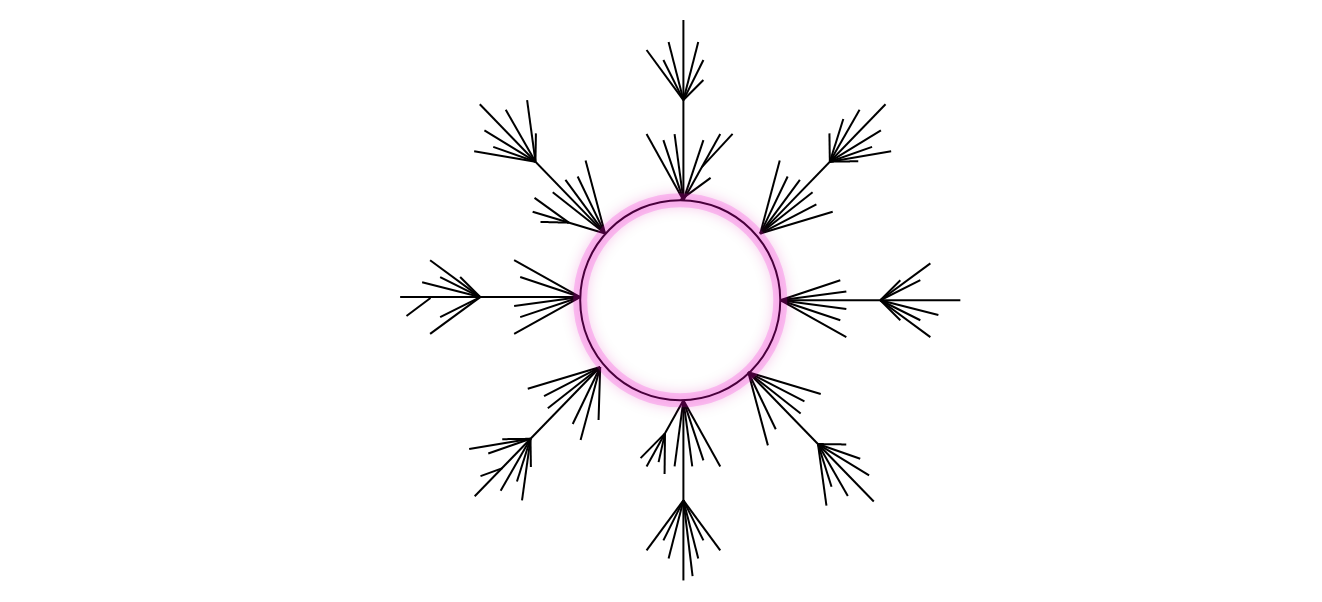
\includegraphics[width=1.0\textwidth]{Images/ellipticcurve.png}
    \caption{A visualisation of the analytification of an elliptic curve with multiplicative reduction.
    The skeleton, which is highlighted here, is a circle.}
    \label{fig:ellipticcurve}
\end{figure}

\section{SNC Models for Elliptic Curves}

\begin{figure}[!ht]
    \centering
    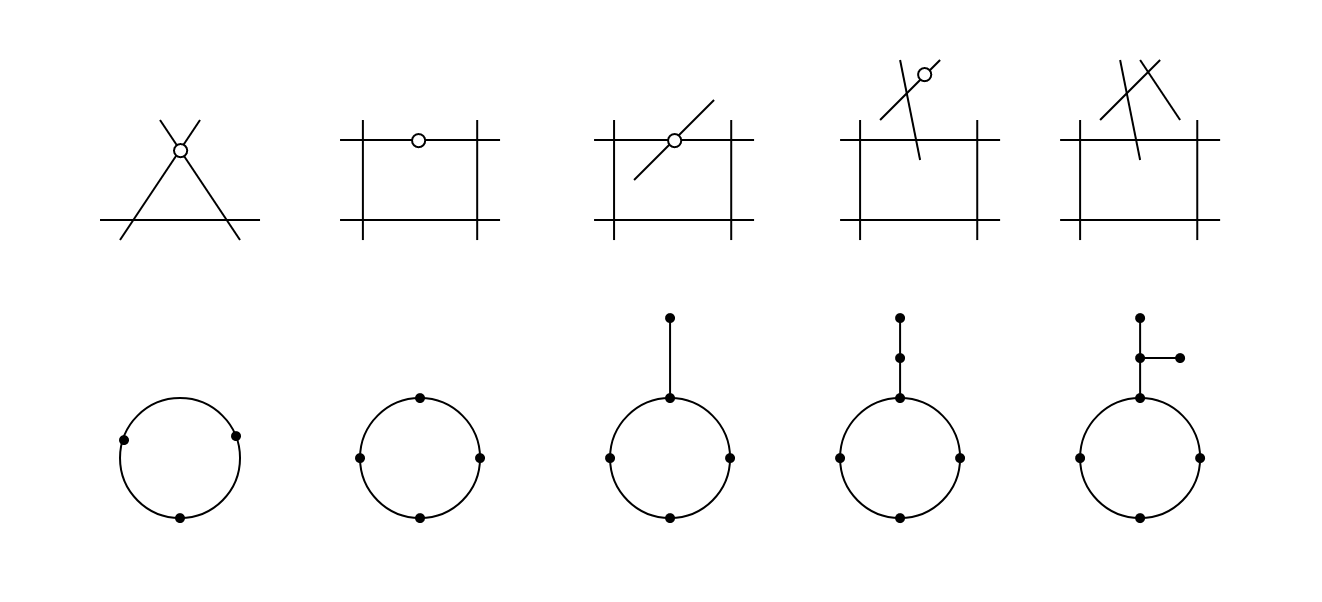
\includegraphics[width=1.0\textwidth]{Images/projectivelimit.png}
    \caption{Diagram indicating how a sequence of point blow-ups of the special fiber affects the skeleton.
    The top row depicts the special fibers of each model, with the next model obtained by a blow-up with the center indicated by a circle.
    The bottom row depicts the dual complex.}
    \label{sequenceofpointblowups}
\end{figure}

We may also consider how the theory of snc models may be used to determine the geometry of the analytification of an elliptic curve $E$ with multiplicative reduction when working over a discrete valuation ring.
In this case, $E$ admits a proper regular model $\model$ over $R$ and
Tate's algorithm may then be used to compute the structure of the special fiber $\model_s$ \parencite[\S IV.9, Theorem 8.2]{silverman}.
Informally, $\model_s$ consists of $n$ rational curves, each appearing with multiplicity one, arranged in the shape of an $n$-gon for some $n \geq 1$.
We assume that $n \geq 2$; then, in such an arrangement, each intersection is transversal, and in particular $\model$ is an snc model for $E$.
The dual graph is then also given by an $n$-gon, hence, it is homeomorphic to a circle once more.
We may recover the full picture of $\anl{E}$ by taking sequences of blow-ups and passing to the projective limit.
This procedure is depicted for $n = 3$ in \cref{sequenceofpointblowups}.
In the general case, we obtain a picture similar to \cref{fig:ellipticcurve}.

A benefit of working with snc models is that we may also investigate the topology of elliptic curves other than those with multiplicative reduction.
We remark that in the case where the elliptic curve $E$ has good reduction, Tate's algorithm indicates that there exists a proper regular model $\model$ where $\model_s$ consists of a single non-singular curve. 
In this case, the dual graph consists of a point, indicating that the space $\anl{E}$ is contractible.


\chapter{Conclusion}

A primary objective of this report was to give an overview of the theory of $k$-analytic spaces and explore methods to construct skeleta, which are a useful tool in analysing the geometry of such spaces.
We break down the evaluation of the contributions of the project by chapter.

We firstly gave an overview of $k$-analytic spaces.
After reviewing the foundational theory, we were able to draw an explicit picture, giving an alternative derivation of Berkovich's classification of points using an approach originally stated in \parencite[Exercise 2.3.3.5]{temk}.
We additionally gave a description of the partial ordering on the affine line; in particular, this involved extending the description given in \parencite{bakernotes} to the case of type IV points, which was left as an exercise.

Next, we considered formal models for analytic spaces and the skeleta of curves over algebraically closed fields.
After giving an overview of the theory of formal schemes, we proved \cref{lemma:affinecaseisaffinoid,separatedix,properisiso}, which detail the relation between the generic fiber of the formal completion and the analytification of the generic fiber.
Following \parencite{bpr}, we developed the theory of semistable vertex sets and sketched the correspondence with semistable formal models of a curve.
We illustrated this correspondence concretely by considering the projective line.

Next, we gave a presentation of the construction of a skeleton for analytic spaces of arbitrary dimension, using snc models.
The main contribution of this section was providing a proof of \cref{thm:homeomorphism}.
The key aspect in showing this result was to prove that for any two distinct points $x$ and $y$ on the analytic space, there exists an snc model such that $x$ and $y$ retract to distinct points on the associated skeleton.
This was shown in \cref{injectivity}, which applied to arbitrary dimension but required resolution of singularities.
Hence, in the case of curves, we also provided a more direct argument utilising only blow-ups with centers given by closed points.

Finally, we exemplified the theory by applying these techniques to the analytification of an elliptic curve.

Berkovich spaces are used prominently in various areas of mathematics.
One particularly exciting application is to mirror symmetry, which is a geometric duality with roots in string theory.
The SYZ conjecture is an attempt to provide mathematical foundations for mirror symmetry, which is originally a physical phenomenon, and in \parencite{kontsevich}, the theory of Berkovich spaces is a central in finding a non-Archimedean analog for the conjecture.
The notion of the skeleton is then a vital component of the conjecture, and in particular, the conjecture is exemplified through the Tate elliptic curve \parencite{vietnam}.
Due to time constraints, we were not able to provide an exposition of this, but it is indubitable that a discussion of such applications would have provided strong motivations for the theory.

Throughout the report, proofs were occasionally omitted when it was deemed that they would not be beneficial in our goals of developing intuition and an understanding of the theory.
In certain cases, we endeavoured to replace the proofs with examples, as in the case of \cref{semistablecorrespondence} and \cref{blowupintersectionskeleton}. 

A possible extension to the work presented here would be to investigate the results in \cref{chapter4} in the context where the base field is algebraically closed.
One effect of the discretely valued assumption was that it simplified certain aspects, such as by ensuring that the schemes we were considering were locally Noetherian.
In particular, the notion of an snc divisor is ill-defined and we must instead work with semistable models.
The construction of monomial and divisorial points, as found in \parencite{MN}, was also presented in the discretely valued case and would first need to be extended to the algebraically closed case.
We must be careful to consider blow-ups with centers given by finitely generated ideals;
we conjecture that the proof of \cref{injectivity} may be extended without too much difficulty, but the analogue of \cref{injectivityforcurves} may be more challenging in this context.

\paragraph{Ethical Considerations}

The ethical concerns regarding this project are negligible, which is highly theoretical in nature. 
One aspect which may be considered is that of the role of areas of mathematics such as number theory in military applications, primarily as a result of its use in cryptography. 
While algebraic geometry and the theory of Berkovich spaces has some uses in the fields of algebraic number theory and arithmetic geometry, the contents of this project are sufficiently detached from any potential applications in real world scenarios for this to be a reasonable concern. 
Additionally, the project does not involve the collection and processing of user data, and does not involve human or animal participants.
The project has not encountered legal or moral issues.


% Vancouver referencing
\printbibliography

\end{document}
